\documentclass[12pt]{report}
% note that the documentclass can take other option such as
% twoside - for double sided printing
% openright - if double side  chapters always start on odd pages
% openany - if double side chapters start on the next page even or odd
% 12pt can be replaced by 11pt

\usepackage[online]{suthesis-2e}
% options are
% online - now the default
% hardcopy - turns off online includes signature page and copyright page in file 
% engineer - does an engineer thesis instead of a PhD dissertation

%% load other packages you need
\usepackage[hidelinks]{hyperref}
\usepackage{amsmath}
\usepackage{amsfonts}
\usepackage{amssymb}
\usepackage[capitalize]{cleveref}
\usepackage{amsthm}
\usepackage{thmtools}
\usepackage{thm-restate}
\usepackage{algorithm}
\usepackage[noend]{algpseudocode}
\usepackage{graphicx}
\usepackage{subcaption}
\usepackage[per-mode=symbol]{siunitx}
\usepackage{booktabs}
\usepackage[usenames,dvipsnames]{xcolor}
\usepackage{tabularx}
\usepackage{rotating}
\usepackage{todonotes}
\usepackage{standalone}
\usepackage{pgfplots}
\usepackage{listings}
\usepackage{float}

\renewcommand\algorithmicthen{}
\renewcommand\algorithmicdo{}

\pgfplotsset{every axis/.append style={font=\footnotesize,legend cell align=left}}

\usepackage[natbib,
            bibstyle=ieee,
            maxnames=6,
            sorting=nyt,
            doi=false,
            backref=true,
            isbn=false
           ]{biblatex}

\AtEveryBibitem{
	\ifentrytype{inproceedings}{
		\clearfield{url}  
		\clearfield{doi}  
	}{}
}


\addbibresource{ref.bib}
\addbibresource{behavior_ref.bib}
\addbibresource{asl_main.bib}
\addbibresource{new.bib}

\sisetup{group-separator={,}}

%% uncomment the following and create mythesis-macros.sty for all your
%% own macros.  This keeps this top level file looking fairly neat.
% \usepackage{mythesis-macros}
\newcommand{\intrid}{\mathrm{i}}
\newcommand{\ownid}{\mathrm{o}}
\newcommand{\intr}[1]{\ensuremath{#1^{(\intrid)}}}
\newcommand{\own}[1]{\ensuremath{#1^{(\ownid)}}} 
\newcommand{\either}[1]{\ensuremath{#1^{(\cdot)}}}
\newcommand{\is}{\ensuremath{\intr{s}}}
\newcommand{\rs}{\ensuremath{\own{s}}}
\newcommand{\psires}{\ensuremath{\own{\psi}_\mathrm{resolution}}}
\newcommand{\psigoal}{\own{\psi}_\mathrm{goal}}
\newcommand{\sterm}{\ensuremath{s_{\mathrm{term}}}}
\newcommand{\tmin}{\ensuremath{t_{\min}}}
\newcommand{\psicand}{\own{\psi}_{\mathrm{cand}}}
\newcommand{\dgoal}{\ensuremath{D_\mathrm{goal}}}
\newcommand{\dnmac}{\ensuremath{D_\mathrm{NMAC}}}
\newcommand{\dev}{\ensuremath{\mathrm{dev }}}
% \newcommand{\argmax}[1]{\underset{#1}{\operatornamewithlimits{argmax}}}
% \newcommand{\argmin}[1]{\underset{#1}{\operatornamewithlimits{argmin}}}
\newcommand{\real}{{\mathbb{R}}}
\renewcommand{\natural}{{\mathbb{N}}}
\newcommand{\naturals}{\natural}
\newcommand{\Beta}{B}

\newcommand{\beh}{\theta}
\newcommand{\Beh}{\Theta}
\newcommand{\phys}{\ensuremath{q}}
\newcommand{\dt}{\ensuremath{\Delta t}}
\newcommand{\bmax}{\ensuremath{b_\text{max}}}
\newcommand{\ith}[1]{{#1}_i}
\newcommand{\jth}[1]{{#1}_j}
\newcommand{\ego}[1]{{#1}_e}
\newcommand{\av}{ego} % used when referring to the ego vehicle in the text

\newcommand{\diro}[1]{{#1}_\phi}
\newcommand{\tdo}[1]{{#1}_{T\phi}}
\newcommand{\trl}[1]{{#1}_{D}}

% approximately proportional to
\newcommand{\appropto}{\mathrel{\vcenter{
  \offinterlineskip\halign{\hfil$##$\cr
    \propto\cr\noalign{\kern2pt}\sim\cr\noalign{\kern-2pt}}}}}



\newcommand{\argmax}{\operatornamewithlimits{argmax}}
\newcommand{\argmin}{\operatornamewithlimits{argmin}}
\newcommand{\reals}{\ensuremath{\mathbb{R}}}
\newcommand{\sspace}{\ensuremath{\mathcal{S}}}
\newcommand{\aspace}{\ensuremath{\mathcal{A}}}
\newcommand{\ospace}{\ensuremath{\mathcal{O}}}
\newcommand{\tdist}{\ensuremath{\mathcal{T}}}
\newcommand{\odist}{\ensuremath{\mathcal{Z}}}
\newcommand{\reward}{\ensuremath{\mathcal{R}}}

\newcommand{\code}[1]{{\small\ttfamily #1}}



\newcommand{\result}[4]{% args mean, sem, color, len
    $#1\pm#2$ & {\color{green!#3!red}\rule{#4cm}{8pt}}
}
\newcommand{\noresult}{ & }


\declaretheorem[name=Theorem]{theorem}
\declaretheorem[name=Definition]{definition}
\declaretheorem[name=Lemma]{lemma}
\declaretheorem[name=Remark]{remark}

\lstdefinelanguage{Julia}%
{
  keywordsprefix=\@,
  morekeywords={abstract,break,case,catch,const,continue,do,else,elseif,%
    end,export,false,for,function,immutable,import,importall,if,in,%
    macro,module,otherwise,quote,return,switch,true,try,type,typealias,%
      using,while,struct},
     keywordstyle=\bfseries\color{red!55!black},
     classoffset=1,
     morekeywords={Float64, Int64, Bool, Any},
      keywordstyle={\bfseries\color{NavyBlue!75!black}},
      classoffset=0,
   sensitive=true,%
   alsoother={$},%$
   morecomment=[l]\#,%
   morecomment=[n]{\#=}{=\#},%
   morestring=[s]{"}{"},%
   morestring=[m]{'}{'},%
}[keywords,comments,strings]%


\lstset{%
    language         = Julia,
    basicstyle       = \ttfamily,
    keywordstyle     = \bfseries\color{blue},
    stringstyle      = \color{magenta},
    commentstyle     = \bfseries\color{OliveGreen},
    showstringspaces = false,
    gobble=0,
}

\lstdefinestyle{customjulia}{
  belowcaptionskip=1\baselineskip,
  breaklines=true,
  % frame=L,
  xleftmargin=\parindent,
  language=Julia,
  showstringspaces=false,
  basicstyle=\footnotesize\ttfamily,
  commentstyle=\itshape\color{OliveGreen!90!black},
  identifierstyle=\color{black},
  stringstyle=\color{orange},
}

\lstdefinestyle{customasm}{
  belowcaptionskip=1\baselineskip,
  frame=L,
  xleftmargin=\parindent,
  language=[x86masm]Assembler,
  basicstyle=\footnotesize\ttfamily,
  commentstyle=\itshape\color{purple!40!black},
}

\newfloat{lstfloat}{htbp}{lop}
\floatname{lstfloat}{Listing}
\def\lstfloatautorefname{Listing} % needed for hyperref/auroref

\title{Safety and Efficiency in Autonomous Vehicles through Planning with Uncertainty}
\author{Zachary Nolan Sunberg}
\dept{Aeronautics and Astronautics} % default is Computer Science, uncomment for other departments
\principaladviser{Mykel J. Kochenderfer}
% \coprincipaladvisor{}
\firstreader{Marco Pavone}
\secondreader{Mac Schwager}
% \thirdreader{}

%the following command would (if uncommented) allow  only chapter1 and
%chapter2 to be processed
% \includeonly{pomcpow}

% if you feel real savvy use
% \typein{Now put in includeonly}
% the \typein command stops latex at this point and allows you to type
% in a command such as
% \includeonly{chapter3,chapter5}
% this can save some time and means you don't have to edit this file
% as much.


\begin{document}

\beforepreface 

\prefacesection{Abstract}

To be effective, autonomous air and ground vehicles should maintain safety while accomplishing tasks efficiently in terms of time and other resources.
Unfortunately, the objectives of safety and efficiency are fundamentally opposed because safety precautions prohibit some efficient actions.
Moreover, the presence of uncertainty about the environment makes planning safe and efficient actions more difficult.

The Markov decision process (MDP) is a systematic framework for modelling sequential decision problems with outcome uncertainty, and the partially observable Markov decision process (POMDP) adds the additional ability to model state uncertainty.
MDPs and POMDPs are suitable models for a wide range of situations that an autonomous vehicle might face.
However, obtaining the exact solution to a general POMDP is an intractable problem.
This thesis considers approximate MDP and POMDP solutions and seeks to quantify their utility for autonomous vehicles.
Specifically, it contains four contributions.

First, the thesis analyzes the use of a certifiable safety constraint alongside approximate optimization in the context of unmanned aerial vehicle collision avoidance.
In order to ensure safety, aerospace systems have particularly stringent certification requirements that likely preclude approximate randomized planning techniques capable of handling uncertainty.
This work evaluates the performance price that comes with using a simple certified policy and shows that MDP and POMDP optimization can significantly reduce that price and improve both safety and efficiency simultaneously.

The second application chapter considers the effects of modeling uncertainty in a difficult lane changing task for a self-driving car.
Specifically, the research estimates the value of planning with the internal states of other human drivers such as their intentions and dispositions.
While several other researchers have used internal-state-aware planning methods to interact with human drivers in desirable ways, they have not evaluated whether these methods offer a substantial quantitative improvement in performance over conventional approaches.
This thesis shows that, in a simplified simulated setting, planning with internal states using a POMDP formulation can significantly improve both safety and efficiency simultaneously.
Moreover, the thesis describes an experimental method for investigating other cases in which internal-state-aware planning may improve performance.

The benefits of POMDP planning can only be realized with algorithms that can handle real-world domains that are continuous and irregular.
To that end, the third contribution of the thesis is a pair of new algorithms for solving POMDPs with continuous state, action, and observation spaces.
These algorithms are motivated by analysis and numerical experiments that show that leading online POMDP solvers fail on continuous observation spaces because of the following two problems.
First, the large observation space causes policy trees to become too wide and not deep enough.
Second, the number of state particles used to represent beliefs collapses to one, causing overconfidence.
The new algorithms, POMCPOW and PFT-DPW, handle these problems using progressive widening and weighted particle belief representations.
Numerical experiments show that they are able to solve problems where previous methods fail.

The final contribution is a software package, POMDPs.jl, which uses the features of the Julia programming language to bring state-of-the-art POMDP solution methods to bear on problems defined through an interface that provides convenience and flexibility.


% first the preface sections.  

% this includes the file preface.tex which should include the
% following commands
% \beforepreface
% \prefacesection{preface}
% body of the preface
% \include{preface}

% any other preface sections

% the last preface section (e.g., acknowledgement.tex)
% should look like
\prefacesection{Acknowledgements}

The biggest debt of gratitude that I owe to any single person for this thesis is to my advisor, Mykel Kochenderfer.
In my opinion, the most admirable thing about Mykel is not the quality of work that he produces (though that is quite impressive), but his commitment and care for students as researchers and people.
I will always think of his office as one of my favorite places of learning on campus.
He took me on as a student during a time of struggling in my research and helped me finish strong.

I also owe a great deal to Marco Pavone, who was my advisor for the first half of this endeavor.
Additionally, my thanks goes out to Dan DeBra, who brought me here to Stanford, and Suman Chakravorty and Jon Rogers who were instrumental in my early growth as a researcher at Texas A\&M.
I am also thankful to the other members of my defense committee: Mac Schwager, Chris Gerdes, and Dorsa Sadigh.

A PhD is not a disembodied pursuit of knowledge, but a journey undertaken by a human with a heart and soul and flaws and weaknesses.
As such, I must thank my community here at Stanford for their care of me as a human exploring God's creation.
Grace Presbyterian church provided a place of connection and growth for me, and my friends gave me constant support.
In particular, two friends, Jeff Reid and Daniel Galbraith, should be noted for their faithfulness over the entire time I was here.
Moreover, I certainly would not be here without my parents and sister and the rest of my family and friends who have been shaping me for my entire life.

I was fortunate to be a part of two outstanding labs during my time here, the Autonomous Systems Lab and the Stanford Intelligence Systems Lab, both of which gave me comraderie and sharpened my technical skills.
I'll remember both the hard work and fun that I had in these places.

The work in this thesis would not have been possible without the generous financial support that I received from a variety of sources including MIT Lincoln Laboratory, the National Science Foundation, the U.S.\ Naval Research Laboratory, and Toyota Resarch Institute.
I must also recognize the leadership and staff of Stanford University and the Aeronautics and Astronautics department.
They have created a remarkable environment for learning.

% body 
% \include{acknowledgement}

\afterpreface


% now for the body of the thesis, modify the number of these lines as needed

% this includes chapter1.tex which should start with a \chapter{...}
% command 
\chapter{Introduction}

\section{Autonomous Vehicles}

\subsection{A World with Autonomous Transportation}

\begin{itemize}
    \item Better Safety
    \item More Efficiency
    \item Less wasted time and stress
    \item Better access to transportation
\end{itemize}

\subsection{Current Progress}

(Not sure what to say here)

\subsection{Remaining Challenges}

\subsubsection{Technical}
\subsubsection{Legal and Ethical}
\subsubsection{Business}

\section{Decision Making Under Uncertainty}

\subsection{Uncertainty in Decision Making}

\subsubsection{Outcome Uncertainty}
\subsubsection{Model Uncertainty}
\subsubsection{State Uncertainty}

\todo{POMDP methods also require a reward function.
In some cases, constructing the reward function that balances different objectives (e.g., safety and efficiency) is straightforward. However, in other cases, human preferences can be difficult to quantify and encode into a reward function.
For these cases, inverse reinforcement learning can be used to determine a suitable reward function based on data of how human drivers act \cite{levine2012continuous, sadigh2016leverage}.}


\subsection{Markov Decision Processes}

The Markov decision process (MDP) is a mathematical formalism that can represent a wide range of sequential decision making problems. 
In an MDP, an agent takes \emph{actions} that affect the \emph{state} of the system and collects \emph{rewards} based on the state and actions.
The \emph{Markov property} is a key attribute of MDPs which states that the next state depends (possibly stochastically) on the current state and action, and not on any previous states or actions.

Formally, an MDP is defined by the 5-tuple $(\mathcal{S}, \mathcal{A}, \mathcal{T}, \mathcal{R}, \gamma)$.
The state space, $\mathcal{S}$, is the set of all possible states.
The action space, $\mathcal{A}$, is the set of all actions available to the agent.
The transition model, $\mathcal{T}$, represents likelihood of transitions, where $\mathcal{T}(s' \mid s, a)$ denotes the probability that the system will transition to state $s'$ given that action $a$ is taken in state $s$.
The reward function, $\mathcal{R}: \mathcal{S} \times \mathcal{A} \times \mathcal{S} \to \reals$ represents the rewards received while interacting in the environment, where
$\mathcal{R}(s, a, s')$ denotes the reward for transitioning from $s$ to $s'$ when action $a$ is taken.
Finally, $\gamma$ governs how reward is discounted in the future.

The objective in an MDP is to find a policy, $\pi: \mathcal{S} \to \mathcal{A}$, that maps each encountered state to an action and, when $a_t = \pi(s_t)$, maximizes the cumulative expected reward,
\begin{equation} \label{eq:cumulative}
    E\left[\sum_{t=0}^\infty \gamma^t \mathcal{R}(s_t, a_t, s_{t+1}) \right]
\end{equation}
where the subscript $t$ is the time index. The state action value function, $Q(s,a)$, is defined as the expectation of the future cumulative reward given that the agent starts in state $s$, immediately takes action $a$, and then follows the optimal policy.

\subsection{Partially Observable Markov Decision Processes}

A partially observable Markov decision process (POMDP) is similar to and MDP except that the agent cannot directly observe the state.
Instead, the agent only has access to observations that are generated probabilistically based on the actions and latent true states.
A POMDP is defined by the 7-tuple $(\sspace, \aspace, \mathcal{T}, \mathcal{R}, \ospace, \odist, \gamma)$, where $\sspace$, $\aspace$, $\mathcal{T}$, $\mathcal{R}$, and $\gamma$ have the same meaning as in an MDP.
Additionally, $\ospace$, is the observation space, and $\odist$ is the observation model.
$\odist(o \mid s, a, s')$ is the probability or probability density of receiving observation $o$ in state $s'$ given that the previous state and action were $s$ and $a$.

Information about the state may be inferred from the entire history of previous actions and observations and the initial information, $b_0$.
Thus, in a POMDP, the agent's policy is a function mapping each possible history, $h_t = (b_0, a_0, o_1, a_1, o_2, \dots, a_{t-1}, o_t)$ to an action.
In some cases, each state's probability can be calculated based on the history.
This distribution is known as a \emph{belief}, with $b_t(s)$ denoting the probability of state $s$.

The belief is a sufficient statistic for optimal decision making.
That is, there exists a policy, $\pi^*$ such that, when $a_t = \pi^*(b_t)$, the expected cumulative reward or ``value function'' is maximized for the POMDP \cite{kaelbling1998planning,kochenderfer2015decision}.
Given the POMDP model, each subsequent belief can be calculated using Bayes' rule according to
\begin{equation} \label{eqn:update}
    b'(s') = \frac{\int_{s\in\mathcal{S}} \odist(o \mid s, a, s') \mathcal{T}(s' \mid s, a) b(s) ds}
    {\int_{s'\in\mathcal{S}} \int_{s\in\mathcal{S}} \odist(o \mid s, a, s') \mathcal{T}(s' \mid s, a) b(s) ds ds'} \text{.}
\end{equation}
When the state space is discrete, the integrals may be replaced with sums.

\todo{Talk about PSPACE completeness}

\subsubsection{Generative Models}

or many problems, it can be difficult to explicitly determine or represent the probability distributions $\mathcal{T}$ or $\odist$.
Some solution approaches, however, only require samples from the state transitions and observations.
A generative model, $G$, stochastically generates a new state, reward, and observation in the partially observable case, given the current state and action, that is $s', r = G(s,a)$ for an MDP, or $s', o, r = G(s, a)$ for a POMDP.
A generative model implicitly defines $\mathcal{T}$ and $\odist$, even when they cannot be explicitly represented.

\subsubsection{Belief MDP}

Every POMDP is equivalent to an MDP where the state space of the MDP is the space of possible beliefs.
The reward function of this "belief MDP" is the expectation of the state-action reward function with respect to the belief.
The Bayesian update of the belief serves as a generative model for the belief space MDP.

\subsection{Value Iteration}

\subsection{Monte Carlo Tree Search} \label{sec:mcts}

MCTS is an effective and widely studied algorithms for online decision-making \cite{browne2012survey}.
It works by incrementally creating a policy tree consisting of alternating layers of state nodes and action nodes and estimating the state-action value function, $Q(s,a)$, at each of the action nodes.
Only a generative model, $G$, is required by the algorithm.
The tree is constructed by running $n$ Monte Carlo simulations with four phases, although there are many variations of this algorithm.
\begin{enumerate}
    \item \emph{Search}. In the initial phase of the simulation, the policy defined by the tree is used.
        At each state node, a selection criterion based on $Q$ is used to choose a favorable action, and the tree is traversed through the node and to the next state node determined by $G$.
    \item \emph{Expansion}. Eventually, the simulation reaches an action node that does not have any children.
        At this point, a new state is sampled with $G$ and a corresponding node created along with children corresponding to each action. 
    \item \emph{Rollout}. After the expansion step, the simulation is continued with a rollout policy, often consisting of randomly selected actions, until the future accumulated reward will be negligible because of the compounding discount factor.
    \item \emph{Update}. Once the simulation has terminated, the estimates of $Q(s,a)$ at each of the visited action nodes are updated with the discounted reward received during the simulation after visiting the node.
\end{enumerate}
This approach builds a tree asymmetrically favoring regions of the state and action spaces that will be visited when the optimal policy is executed.

\subsubsection{Upper Confidence Trees} \label{sec:uct}

The selection criterion used to choose actions in the search phase is very important.
It must balance favoring actions with large $Q$ values that are expected to yield good results with exploration of new actions.
The most widely used approach for this is known as the upper confidence bound for trees (UCT) algorithm.
At each state node, it chooses the action that maximizes the upper confidence bound
\begin{equation} \label{eqn:ucb}
    UCB(s,a) = Q(s,a) + c \sqrt{\frac{\log N(s)}{N(s,a)}}
\end{equation}
where $N(s,a)$ is the number of times the action node has been visited, $N(s) = \sum_{a \in \mathcal{A}} N(s,a)$, and $c$ is a problem-specific parameter that governs the amount of exploration in the tree.
The second term causes the algorithm to favor actions that have been taken less often.

\subsubsection{Double Progressive Widening} \label{sec:dpw}

In cases where the action and state spaces are large or continuous, the MCTS algorithm will produce trees that are very shallow.
In fact, if the action space is continuous, the UCT algorithm will never try the same action twice (observe that, if $N(s,a) = 0$ then $UCB(s,a)$ in (\ref{eqn:ucb}) is infinite, so untried actions are always favored).
Moreover, if the state space is continuous and the transition probability density is finite, the probability of sampling the same state twice from $G$ is zero.
Because of this, simulations will never pass through the same state node twice and a tree below the first layer of state nodes will never be constructed.

In progressive widening, the number of children of a node is artificially limited to $k N^\alpha$ where $N$ is the number of times the node has been visited and $k$ and $\alpha$ are parameters chosen for the problem \cite{couetoux2011double}.
Originally, progressive widening was applied to the action space, and was found to be especially effective when a set of preferred actions was tried first \cite{browne2012survey}.
The term \emph{double} progressive widening refers to progressive widening in both the state and action space.
When the number of state nodes is greater than the limit, instead of simulating a new state transition, one of the previously generated states is chosen with probability proportional to the number of times it has been previously generated.


\subsection{Particle Filtering} \label{sec:particle}

Aside from a few special cases, for example when the system dynamics are linear and the transition and observation distributions are Gaussian, the integrals in the Bayesian belief update (\ref{eqn:update}) are impossible or difficult to solve analytically.
Thus, numerical approaches must be used.
A popular technique for this is particle filtering, usually incorporating domain-specific heuristic modifications to prevent problems such as particle depletion \cite{thrun2005probabilistic}.

Sequential importance resampling, one of the most common and effective variations, requires a state generative model, $G_s$ that can sample from the transition distribution and an explicit representation of the observation distribution, $\odist(\cdot \mid s, a, s')$, which is often easier to represent than the transition distribution.
The belief is approximated with a set of $m$ particles, $\{s_i\}_{i=1}^m$ and associated weights, $\{w_i\}_{i=1}^m$.
The probability of each state is approximated by the sum of the weights corresponding to particles with that state value,
\begin{equation}
    b(s) \approx \sum_{i=1}^m w_i \delta_s (s_i)
\end{equation}
where $\delta_s(\cdot)$ is the Dirac delta function centered at $s$.
A belief update is approximated by sampling $m$ states $\{\tilde{s}_i\}_{i=1}^m$ from the collection of particles with probability proportional to the associated weight, generating a particle, $s'_i = G(\tilde{s}_i, a)$ for each of these states, and finally setting the new weight proportional to the probability of generating the measured observation with this state, $w'_i \propto \odist(o \mid \tilde{s}_i, a, s'_i)$.

\subsection{Approximate Solutions to POMDPs} \label{sec:solutions}

Considerable progress has been made in solving large POMDPs.
Initially, exact offline solutions to problems with only a few discrete states, actions, and observations were sought by using value iteration and taking advantage of the convexity of the value function \cite{kaelbling1998planning}, although solutions to larger problems were also explored using Monte Carlo simulation and interpolation between belief states \cite{thrun1999monte}.
Many effective offline planners for discrete problems use point based value iteration, where a selection of points in the belief space are used for value function approximation,  \cite{kurniawati2008sarsop}.
Offline solutions for problems with continuous state and observation spaces have also been proposed \cite{bai2014integrated,brechtel2013solving}.

There are also various solution approaches that are applicable to specific classes of POMDPs, including continuous problems.
For example, \citet{platt2010belief} simplify planning in large domains by assuming that the most likely observation will always be received, which can provide an acceptable approximation in some problems with unimodal observation distributions.
\citet{morere2016bayesian} solve a monitoring problem with continuous spaces with a Gaussian process belief update.
\citet{hoey2005solving} propose a method for partitioning large observation spaces without information loss, but demonstrate the method only on small state and action spaces that have a modest number of conditional plans.
Other methods involve motion-planning techniques \cite{melchior2007particle,prentice2009belief,bry2011rapidly}.
In particular, \citet{agha2011firm} present a method to take advantage of the existence of a stabilizing controller in belief space planning.
\citet{van2012motion} perform local optimization with respect to uncertainty on a pre-computed path, and \citet{indelman2015planning} devise a hierarchical approach that handles uncertainty in both the robot's state and the surrounding environment.

General purpose online algorithms for POMDPs have also been proposed.
These algorithms are mostly derivatives of the MCTS algorithm for MDPs (\cref{sec:mcts}).
A conceptually straightforward way to solve a POMDP using MCTS is to apply it to the corresponding belief MDP.
Indeed, many tree search techniques have been applied to POMDP problems in this way \cite{ross2008online}.
However, when the Bayesian belief update is used, this approach is computationally expensive.
POMCP can tackle problems many times larger than its predecessors because it uses state trajectory simulations, rather than full belief trajectories, to build the tree.
Determinized sparse partially observable tree (DESPOT) is a similar approach that attempts to achieve better performance by analyzing only a small number of random outcomes in the tree \cite{somani2013despot}.
Adaptive belief tree (ABT) was designed specifically to accommodate changes in the environment without having to replan from scratch \cite{kurniawati2016online}.

\todo{Add POMCP section(?), or at least specifics}
\todo{Add QMDP-Net}

\subsection{QMDP} \label{sec:qmdp}

\todo{write QMDP section}

\section{Contributions}

\chapter{Trusted and Optimized UAV Collision Avoidance} \label{chap:uav}

This thesis's first investigation into safety and efficiency is in the context of unmanned aerial vehicles (UAVs).
Collision avoidance is an important challenge that must be overcome to make UAV operation routine and safe.
In this chapter,  the suitability of the collision avoidance system for easy certification is the primary safety focus.
The challenge is to create a system that is both easy to certify and has minimal impact on efficient normal operations.


\section{Collision Avoidance for UAVs} \label{sec:uavintro}

As unmanned aerial vehicles (UAVs) move toward full autonomy, it is vital that they be capable of effectively responding to anomalous events, such as the intrusion of another aircraft into the vehicle's flight path. Minimizing collision risk for aircraft in general, and UAVs in particular, is challenging for a number of reasons. First, avoiding collision requires planning in a way that accounts for the large degree of uncertainty in the future paths of the aircraft. Second, the planning process must balance the competing goals of ensuring safety and avoiding disruption of normal operations. Many approaches have been proposed to address these challenges \cite{JKK-LCY:00,HYO-MJK:15,RB-CF-HE:09,GH-RB-JM:11,HH-JJ-CM:10,AN-CM-GD:12,ST-MJK-LPK-TLP-JKK:10,MJK-JPC:11,MJK-JPC-LPK-TL:10,LPK-TL:09,HB-DH-MJK-WSL:12,JEH-MJK-WAO:13,EJR:14}.

At present, there are two fundamentally different approaches to designing a conflict resolution system.The first approach focuses on inspiring confidence and trust in the system by making it as simple as possible for government regulators and vehicle operators to understand.
This is accomplished by constructing the algorithm using hand-specified rules.
Several algorithms that fit this paradigm have been proposed, and research toward formally verifying their safety-critical properties is underway \cite{RB-CF-HE:09,GH-RB-JM:11,HH-JJ-CM:10,AN-CM-GD:12}.  In this chapter, such algorithms are referred to as \emph{trusted resolution logic} (TRL).
Many TRL systems have a number of parameters that determine how conservatively the system behaves.
These parameters may be tuned to meet specific performance goals, but their exact effects on performance can typically only be characterized empirically.

The second approach focuses on optimizing performance.
This entails the offline or online  computation of a ``best" response action. Dynamic programming is widely used for this task \cite{ST-MJK-LPK-TLP-JKK:10,MJK-JPC:11,MJK-JPC-LPK-TL:10,LPK-TL:09,HB-DH-MJK-WSL:12,JEH-MJK-WAO:13}. 
Conflict resolution systems designed using this approach will be referred to as \emph{directly optimized} systems. 
Unfortunately, even if a conflict resolution system performs well in simulation, government regulators and vehicle operators will often (and sometimes rightly) be wary of trusting its safety due to perceived complexity and unpredictability.
Even in the best case, such a system would require expensive and time-consuming development of tools for validation as was the case for the recently developed replacement for the traffic alert and collision avoidance system (TCAS) \cite{JEH-MJK-WAO:13}. 

This chapter proposes two conflict resolution strategies that combine the strengths of trusted resolution logic and direct optimization approaches.
In both strategies, dynamic programming is used to find near-optimal actions for each state.
The difference lies in the set of actions available to the optimizer.
In the \emph{optimized TRL} approach, the actions are a set of certified TRL parameters.
In the \emph{trusted direct optimization} approach, the actions are a state-dependent set of immediate response actions that are deemed safe by certified TRL.
Both strategies may achieve better performance than the base TRL without becoming significantly more difficult to certify.

\begin{figure}
    \centering
    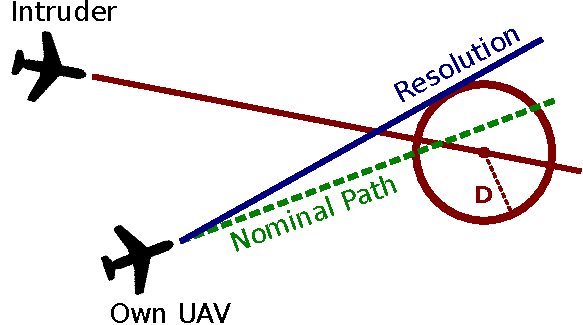
\includegraphics[height=5.0cm]{media/simple_trl.pdf}
    \caption[Trusted resolution logic]{Trusted resolution logic. The near mid air collision exclusion zone (circle with radius $D$) moves with the intruder through time, but is shown here only at the time of closest approach. The TRL (\Cref{alg:trl}) finds a straight trajectory close to the nominal path that avoids this zone.}
    \label{fig:trl}
\end{figure}

The new approaches are tested in a scenario containing a UAV equipped with a perfect (noiseless) sensor to detect the state of an intruder and a simple reference TRL to resolve conflicts. This TRL, illustrated in \Cref{fig:trl}, determines a path that does not pass within a specified separation distance, $D$, of the intruder given that the intruder maintains its current heading (except in cases where no such path exists or when the TRL's heading resolution is too coarse to find such a path).
This reference TRL is described in more detail in \Cref{sec:trl}.

To account for uncertainty in the intruder's flight path, if $D$ takes a constant value, say $\bar{D}$, the value must be increased to ensure safety, but this may cause unnecessary departures from normal operation.
To overcome this limitation and ensure safety without being too conservative, implementations of the two strategies mentioned above are applied.
The optimized TRL approach computes a policy, $\trl{\pi}$, that specifies a time varying separation distance, $D_t$, for each encounter state, while the direct optimization and trusted direct optimization approaches compute policies, $\diro{\pi}$ and $\tdo{\pi}$, that specify a bank angle, $\phi_t$ for each encounter state.
For this reason, symbols referring to the optimized TRL approach generally have subscript $D$, while those referring to direct optimization and trusted direct optimization have a subscript $\phi$.

The problem of dynamically selecting actions $D_t$ or $\phi_t$ can be formulated as a Markov decision process (MDP). Online solution of $\trl{\pi}$, $\diro{\pi}$, or $\tdo{\pi}$ using an algorithm such as Monte Carlo Tree Search (MCTS) \cite{couetoux2011double} would be conceptually straightforward, but would require significant computing power onboard the vehicle, and it would be difficult and time-consuming to rigorously certify the implementation of MCTS due to its reliance on pseudo-random number generation. A key contribution of this chapter is to devise an offline approach to compute the policies. Offline optimization is difficult because of the size of the state space of the MDP, which is the Cartesian product of the continuous state spaces of the UAV and the intruder. This challenge is overcome with a value function approximation scheme that uses grid-based features that exploit the structure of the state space. This value function is optimized using simulation-based approximate value iteration.


\section{MDP Models}\label{sec:uavmodel}

The problem of avoiding an intruder using one of the strategies above is formulated as an MDP, referred to as an \emph{encounter MDP}. An encounter involves two aerial vehicles flying in proximity. The first is the vehicle for which the resolution controller is being designed, which will be referred as the ``own UAV" (or simply ``UAV''). The second is the intruder vehicle, which may be manned or unmanned and will be referred to as the ``intruder". Specifically, the encounter MDP is defined by the tuple $(\sspace, \aspace, \tdist, R)$, which consists of

\begin{itemize}
    \item The state space, $S$: The state of the encounter, $s$, consists of (1) the state of the own UAV, $\rs$, (2) the state of the intruder, $\is$, and (3) a boolean variable $\dev$. The variable $\dev$ is set to true if the UAV has deviated  from its nominal course. Collectively, the state is given by the triple
        \begin{equation}
            s = \left(\rs, \is, \dev\right) \text{.}
        \end{equation}
        The state components $\rs$ and $\is$ are specified in Section \ref{sec:veh}.
        To model termination, the state space $S$ includes a ``dummy" termination state, denoted with $\sterm$.
    \item The action space, $A$: The action space differs for the two approaches as described in detail in \Cref{sec:aspaces}. $a$ will be used to refer to all types of action depending on the context.
    \item The state transition probability density function, $T: S \times A \times S \to \mathbb{R}$: The value $T(s,a,s')$ is the probability density of transitioning to state $s'$ given that action $a$ is taken at state $s$. This function is implicitly defined by a generative model that consists of a state transition function $F(\cdot)$ (described in \Cref{sec:control}) and a stochastic process $W$ (described in \Cref{sec:veh}).
    \item The reward, $\reward:\sspace \times \aspace \to \reals$: The reward function, defined in \Cref{sec:rew}, rewards reaching a goal and penalizes near mid air collisions (NMACs), deviation from the nominal path, and time outside a goal region.
\end{itemize}

\subsection{Model Assumptions}\label{sec:assumptions}

% SHORTEN: this could be more concise
Two important simplifying assumptions were made for this initial study. First, the UAV and the intruder move only in the horizontal plane and at constant speed. Modeling horizontal maneuvers is necessary because UAVs will likely have to employ horizontal maneuvers in place of or in addition to the vertical maneuvers that current collision avoidance systems for manned aircraft such as TCAS rely on. This is due to both climb performance limitations and regulatory constraints such as the \num{400}\si{ft} ceiling for small (\num{<55}\si{lb}) commercial UAVs in Federal Aviation Administration rules \cite{faa2018small}. Constraining altitude and speed simplifies exposition and reduces the size of the state space, keeping the computational burden modest compared with a formulation that includes variable altitude and speed. Extensions to higher fidelity models (e.g.,~\cite{MJK-MWME-LPE-JKK-JDG:10}) are possible and left for future research.
A higher fidelity model would present a computational challenge, but perhaps not an insurmountable one.
For example, the TRL could be extended to handle variable speed and altitude, but the policy could be optimized only on the most important dimensions of the model (e.g., the horizontal plane). See~\cite{MJK-JPC-PPR:10} for a similar successful example.

Second, the intruder dynamics are independent of the UAV's state; in other words, the intruder does not react to the flight path of the UAV. The cooperative setting where both the UAV and the intruder are equipped with a collision avoidance system (CAS) \cite{EJR:14,CT-GJP-SSS:98,MJK-JPC:11} is left for future research.

\subsection{Vehicle States and Dynamics}\label{sec:veh}

This paper uses a very simple discrete-time model of an encounter between two aerial vehicles with time steps of duration $\Delta t$. Throughout this section, the superscripts $\own{}$ and $\intr{}$ refer to the own UAV and intruder quantities, respectively, while the superscript $\either{}$ may be replaced by either $\own{}$ or $\intr{}$. Both the UAV's and the intruder's states consist of the horizontal position $(x,y)$ and heading $\psi$, that is
\begin{equation}
    \rs = \left(\own{x}, \own{y}, \own{\psi} \right)\text{,} \quad 
    \is = \left(\intr{x}, \intr{y}, \intr{\psi} \right)\text{.}
\end{equation}
The UAV and intruder also have similar dynamics. Both aircraft fly forward in the horizontal plane at constant speeds denoted by $\either{v}$. They may turn at rates $\either{\dot{\psi}}$ that remain constant over the simulation step. The following equations define the vehicle dynamics: 
\begin{align*}
    \either{x}_{t+1} &= \begin{cases}
        \either{x}_{t} + \either{v} \cos\left(\either{\psi}_t\right)\Delta t & \text{if } \either{\dot{\psi}} = 0 \\
        \either{x}_{t} + \either{v} \frac{\sin\left( \either{\psi}_t + w_t\Delta t \right) - \sin\left( \either{\psi}_t \right)}{\either{\dot{\psi}}} & \text{otherwise}\\
    \end{cases} \\
    \either{y}_{t+1} &= \begin{cases}
        \either{y}_{t} + \either{v} \sin\left(\either{\psi}_t\right)\Delta t & \text{if } \either{\dot{\psi}} = 0 \\
        \either{y}_{t} - \either{v} \frac{\cos\left(\either{\psi}_t + \either{\dot{\psi}}\Delta t\right) - \cos\left(\either{\psi}_t\right)}{\either{\dot{\psi}}} & \text{otherwise}\\
    \end{cases} \\
    \either{\psi}_{t+1} &= \either{\psi}_t + \either{\dot{\psi}} \Delta t \text{.}
\end{align*}

The intruder makes small random turns with
\begin{equation}
    \intr{\dot{\psi}} = w_t \text{,}
\end{equation}
where $w_t$ is a stochastic disturbance. We let $W$ denote the stochastic process $\{w_t: t\in \naturals\}$. The random variables $w_t$ in $W$ are assumed independent and identically normally distributed with zero mean and a specified standard deviation, $\sigma_{\dot{\psi}}$. Subsequently, the intruder dynamics will be collectively referred to as $\intr{f}$ so that
\begin{equation} \label{eq:idyn}
    \intr{s_{t+1}} = \intr{f}\left(\intr{s}_t, w_t\right) \text{.}
\end{equation}


The dynamics of the  UAV are simplified conventional fixed wing aircraft dynamics with a single input, namely the roll angle $\own{\phi}$. We assume that the roll dynamics are  fast compared to the other system dynamics, so that the roll angle $\own{\phi}$  may be directly and instantaneously commanded by the control system. This assumption avoids the inclusion of roll dynamics, which would increase the size of the state space.
\begin{equation}
    \own{\dot{\psi}_t} = \frac{g \tan \own{\phi}_t}{\own{v}} \text{,}
\end{equation}
where $g$ is acceleration due to gravity. The performance of the UAV is limited by a maximum bank angle
\begin{eqnarray}
    |\own{\phi}_t| \leq \phi_\text{max} \text{.}
\end{eqnarray}
The UAV dynamics will be collectively referred to as $\own{f}$, and
\begin{equation} \label{eq:odyn}
    \own{s_{t+1}} = \own{f}\left(\own{s}_t, \own{\phi}_t\right) \text{.}
\end{equation}

\subsection{Transition Function} \label{sec:control}

It will often be convenient to refer to all of the dynamics in the state transition with a single transition function, which will be defined below after defining additional behavior regarding goals and near mid-air collisions.

The goal region that the UAV is trying to reach is denoted by $S_\text{goal}$. This is the set of all states in $S$ for which $\left\|\left(\own{x}, \own{y}\right) - \left(\own{x}_{\text{goal}}, \own{y}_{\text{goal}}\right)\right\| \leq \dgoal$, where $\dgoal>0$ is a specified goal region radius, and $\left(\own{x}_{\text{goal}}, \own{y}_{\text{goal}}\right)$ is the goal center location.
A near mid air collision (NMAC) occurs at time $t$ if the UAV and intruder are within a minimum separation distance, $\dnmac > 0$, that is if $\left\|\left(\own{x}_t, \own{y}_t\right) - \left(\intr{x}_t, \intr{y}_t\right)\right\| \leq \dnmac$.
If the UAV reaches the goal region at some time $t$, i.e., $s_t \in S_\text{goal}$, or if an NMAC occurs, the overall encounter state $s$  transitions to the terminal state $\sterm$ and remains there.  If the UAV performs a turn, $\dev$ is set to true because the vehicle has now deviated from the nominal straight path to the goal.

Let the state transition function, defined by \eqref{eq:idyn}, \eqref{eq:odyn}, and the special cases above, be denoted concisely as $F$ so that  
\begin{equation}\label{eq:sys_dyn}
    s_{t+1} = F(s_t, \own{\phi}_t, w_t) \text{.}
\end{equation}


\subsection{Reference Trusted Resolution Logic}\label{sec:trl}

The numerical tests use the simple reference TRL shown in \cref{fig:trl}.
The TRL determines a heading angle, $\psires$, that is close to the heading to the goal, $\psigoal$, and that will avoid future conflicts with the intruder given that the intruder maintains its current heading. This is shown in Figure~\ref{fig:trl}.

\subsubsection{Minimum Separation Distance}

Given an initial state $s$, a candidate heading for the UAV, $\psicand$, and that both vehicles maintain their heading, the distance between the vehicles at the time of closest approach is a simple analytical function. Specifically, consider the distance  $d\left(s,\psicand,\tau\right)$ between the vehicles $\tau$ time units in the future, i.e., 
\begin{equation} \label{eqn:dist}
    d\left(s, \psicand, \tau\right) = \sqrt{\Delta x(\tau)^2 + \Delta y(\tau)^2} \text{,}
\end{equation}
where
\begin{align*}
    \Delta x(\tau) &= \intr{x} - \own{x} + \tau \intr{v} \cos\left(\intr{\psi}\right) - \tau \own{v} \cos\left(\psicand\right),\\
    \Delta y(\tau) &= \intr{y} - \own{y} + \tau \intr{v} \sin\left(\intr{\psi}\right) - \tau \own{v} \sin\left(\psicand\right) \text{.}
\end{align*}

The minimum distance between the two vehicles is analytically found by setting the time derivative of $d\left(s,\psicand, \tau\right)$ to zero. Specifically, the time at which the vehicles are closest is given by
\begin{equation}
    \tau_\text{min}\left(s,\psicand\right) = \max \left\{\frac{a + b}{c-2d}, 0\right\} \text{,}
\end{equation}
where
\begin{align*}
    a &:= -\intr{v}\intr{x} \cos(\intr{\psi}) - \intr{v} \intr{y} \sin(\intr{\psi}) \\
    b &:= \own{v} \intr{x} \cos(\psicand) + \own{v} \intr{y} \sin(\psicand) \\
    c &:= v^{(\ownid)\,2} + v^{(\intrid)\,2}\cos^2(\intr{\psi}) + v^{(\intrid)\,2}\sin^2(\intr{\psi}) \\
    d &:= \own{v}\intr{v} ( \cos(\intr{\psi})\cos(\psicand) + \sin(\intr{\psi})\sin(\psicand) ) \text{.}
\end{align*}
The minimum separation distance over all future time is then
\begin{equation}
    d_\text{min}\left(s, \psicand\right) := d\left(s, \psicand, \tau_\text{min}\left(s,\psicand\right)\right) \text{.}
\end{equation}

It will also be occasionally convenient to use $d_\text{min}$ with only a state as an argument.
In this case, $\psicand$ should be understood to be the UAV heading angle corresponding to that state, that is $d_\text{min}(s) := d_\text{min}(s, \own{\psi})$ where $\own{\psi}$ is the UAV heading in $s$.

\subsubsection{Discrete Heading Optimization}

The TRL begins with a discrete set of potential heading values (each denoted $\psicand$) for the UAV. It then determines, for a desired separation distance $D$,  which of those will not result in a collision given that the UAV and  intruder maintain their headings. Finally, it selects the value from that set which is closest to $\psigoal$. The TRL is outlined in \cref{alg:trl}.

\renewcommand{\algorithmicrequire}{\textbf{Input:}}
\renewcommand{\algorithmicensure}{\textbf{Output:}}
\begin{algorithm}[tbhp]
    \caption{Trusted Resolution Logic}\label{alg:trl}
\begin{algorithmic}
    \Require Encounter state $s$, desired separation distance $D$
    \Ensure Resolution heading angle $\psires$
        \Function{$\text{TRL}$}{$s$, $D$}
        \State $\Psi \gets \left\{\own{\psi} + n\pi/N : n \in \{-N,\ldots,N\} \right\}$
        \Comment{range of values for heading}
        \State $D^* = \underset{\psicand \in \Psi}{\max}\, d_\text{min}\left(s, \psicand\right)$
        \If{$D^*< D$} \Comment{conflict inescapable}
            \State $\Psi \gets \left\{\psicand \in \Psi : d_\text{min}\left(s, \psicand\right) = D^*\right\}$
            \State \Return $\underset{\psicand \in \Psi}{\argmin}\,|\psicand-\psigoal|$
        \Else
            \State $\Psi \gets \left\{\psicand \in \Psi : d_\text{min}\left(s, \psicand\right) \geq D\right\}$
            \State \Return $\underset{\psicand \in \Psi}{\argmin}\,|\psicand-\psigoal|$
        \EndIf
    \EndFunction
\end{algorithmic}
\end{algorithm}


\subsection{Action Spaces and Control Systems}\label{sec:aspaces}

The numerical experiments consider policies generated by solving three different MDPs, each with a different action space. 
For the sake of conciseness, $a$ will be used to represent any type of action depending on the context.

\subsubsection{Direct Optimization}

In the direct optimization approach, the actions are simply the bank angles less than $\phi_\text{max}$, that is $\diro{\aspace} = \left\{\phi \in \reals: |\phi| \leq \phi_\text{max} \right\}$.

\subsubsection{Trusted Direct Optimization}

In the trusted direct optimization approach, the set of actions is state dependent.
Specifically, it is the set of bank angles that the TRL deems safe, that is $\tdo{\aspace}(s) = \left\{\phi \in \diro{\aspace}: d_\text{min}(F(s, \phi, 0)) > D_\text{NMAC} \right\}$.

\subsubsection{Optimized TRL}

In the optimized TRL approach, the actions are the possible values for the separation distance, that is $\trl{\aspace} = D\in \reals_{\geq 0}$ used in the TRL (see Figure \ref{fig:trl}).
A simple low level control system converts the desired heading from the TRL (denoted $\psires$) and into a bank angle for the vehicle.
This is denoted with
\begin{equation}
    \own{\phi}_t = c\left(\own{s}_t, \psires \right) \text{,}
\end{equation}
where $c(\cdot)$ represents the low level controller.
When the action is a separation distance, the transition function, $F$, should be understood to contain the TRL and low level control system, that is
\begin{equation}
    F(s_t, D_t, w_t) := F(s_t, c(\own{s}_t, \text{TRL}(s_t, D_t)), w_t) \text{.}
\end{equation}

\subsection{Reward}\label{sec:rew}

This section considers optimization of two competing metrics. The first goal is to minimize the risk of a NMAC. This aspect of performance is quantified with the fraction of NMACs prevented. The second goal is to minimize the probability of deviation from the nominal path. This metric was chosen (as opposed to a metric that penalizes the size of the deviation) because, in a commercial setting, any deviation from the normal operating plan might have a large cost in the form of disrupting schedules, preventing a mission from being completed, or requiring manual human monitoring. The MDP reward function is designed to encourage the policy towards a solution that performs well with respect to these goals.  

Specifically, the utility associated with an encounter is the sum of the stage-wise rewards throughout  the entire encounter
\begin{equation}\label{eqn:encrew}
    \sum_{t=0}^\infty \reward(s_t, a_t) \text{.}
\end{equation}

In order to meet both goals, the stage-wise reward is
\begin{align}\label{eqn:rew}
    \reward(s_t, a_t) := & - c_\text{step} + r_\text{goal} \times \operatorname{in\_goal}\left(\own{s}_t\right) \nonumber\\
             & - c_\text{dev} \times \operatorname{causes\_deviation}(s_t, a_t) \nonumber\\
             & - \lambda \times \operatorname{is\_NMAC}(s_t) \text{,}
\end{align}
for positive constants $c_\text{step}$, $r_\text{goal}$, $c_\text{dev}$,  and $ \lambda$. The first term is a small constant cost accumulated in each step to push the policy to quickly reach the goal. The function $\operatorname{in\_goal}$ indicates that the UAV is within the goal region, so the second term is a reward for reaching the goal. The third term is a penalty for deviating from the nominal path. The function $\operatorname{causes\_deviation}$ returns $1$ if the action will cause a deviation from the nominal course and $0$ otherwise. It will only return $1$ if the vehicle has not previously deviated and $\dev$ is false, so the penalty may only occur once during an encounter. This behavior makes the inclusion of $\dev$ in the state necessary. Constants $c_\text{step}$, $r_\text{goal}$, and $c_\text{dev} $ represent relative weightings for the terms that incentivize a policy that reaches the goal quickly and minimizes the probability of deviation. Example values for these constants  are given in \Cref{sec:results}. The fourth term is the cost for a collision. The weight $\lambda$ balances the two performance goals. We heuristically expect there to be a value of $\lambda$ for which the solution to the MDP meets the desired risk ratio if it is attainable. Bisection, or even a simple sweep of values can be used to find a suitable value, and this method has been used previously to analyze the performance of aircraft collision avoidance systems \cite{HB-DH-MJK-WSL:12,MJK-JPC:11}.

\subsection{Problem statement}
The problem we consider  is to find a feedback control policy $\pi^*: S \to A$, mapping an encounter state $s_t$ into an action $a_t$,  that maximizes the expected reward \eqref{eqn:encrew} subject to the system dynamics \eqref{eq:sys_dyn}:
\begin{equation}\label{eq:prob}
\begin{aligned}
& \underset{\pi}{\text{maximize}}
& & E \left[\sum_{t=0}^\infty \reward(s_t, \pi(s_t))\right] \\
& \text{subject to}
& & s_{t+1} = F(s_t, \pi(s_t), w_t) \text{,}
\end{aligned}
\end{equation}
for all initial states $s_0 \in S$. To make the solution of problem \eqref{eq:prob} practical, we present an approximate dynamic programming approach that yields a suboptimal policy, $\tilde{\pi}$, in the next section.

\section{Solution Approach} \label{sec:approach}

Since the problem \eqref{eq:prob} has continuous state and action spaces and complex dynamics, it is difficult to solve.
In order to make it more tractable, two approximations are used.

First, only a small number of discrete actions, which will be referred to as $\tilde{\aspace}$, are considered. Specifically, for the optimized TRL, direct optimization, and trusted direct optimization approaches, the following action spaces are used:
\begin{align}
    \trl{\tilde{\aspace}} &= \{\dnmac, \allowbreak 1.5 \dnmac, \allowbreak 2 \dnmac, \allowbreak 3 \dnmac, \allowbreak 4 \dnmac \} \\
    \diro{\tilde{\aspace}} &= \left\{-\phi_\text{max},-\frac{\phi_\text{max}}{2}, 0, \frac{\phi_\text{max}}{2},\phi_\text{max}\right\} \\
    \tdo{\tilde{\aspace}}(s) &= \left\{\phi \in \diro{\tilde{\aspace}} : d_\text{min}\left(F(s, \phi, 0)\right) > D_\text{NMAC} \right\} \text{.}
\end{align}

The second approximation is the approximate value iteration algorithm \cite{DB:05} used to optimize the policy. The value function, $V$, represents the expected value of the future reward given that the encounter is in state $s$ and an optimal policy will be executed in the future. We approximate $V$ with a linear architecture of the form
\begin{equation}\label{eqn:val}
    \tilde{V}(s) = \beta(s)^\top \theta \text{,}
\end{equation}
where the feature function $\beta$ returns a vector of $N_\beta$ feature values, and $\theta\in \reals^{N_\beta}$ is a vector of weights \cite{DB:05}. At each step of  value iteration, the weight vector $\theta$ is fitted to the results of a large number of single-step simulations by solving a linear least-squares problem. After value iteration has converged, $\tilde{V}$ is used to estimate a \emph{post-decision state} value function, $\tilde{V}_q$,  which is also approximated using a linear combination of features. The policy is extracted online in real time by selecting the action that results in the post-decision state that has the highest value according to $\tilde{V}_q$. The choice of working with post-decision states will be discussed in \Cref{sec:extract}.

\subsection{Approximate Value Iteration} \label{sec:iter}

The bulk of the computation is carried out offline before vehicle deployment using simulation. Specifically, the first step is to estimate the optimal value function for problem \eqref{eq:prob} using value iteration \cite{DB:05}. On a continuous state space such as the encounter state space used in this work, the Bellman operator used in value iteration cannot be applied for each of the uncountably infinite number of states, so an approximation must be used.

In this paper we adopt projected value iteration \cite{DB:05}. 
In this algorithm, each successive value function approximation, $\tilde{V}_k$, is the result of the Bellman operation projected onto a linear subspace with respect to the Euclidean norm, that is
\begin{equation}\label{eqn:projvi}
    \tilde{V}_{k+1}(s) = \Pi \mathcal{B}[\tilde{V}_k](s) \text{,}
\end{equation}
where $\mathcal{B}$ is the Bellman operator, and $\Pi$ is a projection onto the linear subspace $\Phi$ spanned by the $N_\beta$ basis functions (see \cite{DB:05} for a detailed discussion of this approach).

Two important factors that make projected value iteration an attractive option compared to other approaches, in particular deep reinforcement learning~\cite{mnih2015human}, are the following:
% First, the ability to simulate independent transitions from arbitrary states with a generative model allows value iteration to be used rather than episode-based reinforcement learning where decorrelating data is an additional step.
First, since it is relatively easy to choose a feature set that yields acceptable performance by hand (see \cref{sec:features}), more flexible function approximation approaches that also learn features, such as deep neural networks~\cite{goodfellow2016deep}, are not necessary.
Second, the least squares optimization problem solved at each iteration of projected value iteration (\ref{eq:leastsq}) requires much less computation than the gradient descent required to train a neural network.
% \footnote{Another factor contributing to this decision was that, at the time this research was originally conducted, the computational frameworks that are now commonly used for training neural networks were not yet mature.}

Monte Carlo simulations are used to perform the approximate value iteration \eqref{eqn:projvi}. Specifically, for each iteration, $N_\text{state}$ states are uniformly randomly selected. If the states lie within the grids used in the feature function (see \Cref{sec:features}) the sample is ``snapped'' to the nearest grid point to prevent approximation errors due to the Gibbs phenomenon \cite{JF-FBR:91}. At each sampled state $s^{[n]}$, $n=1,\ldots, N_\text{state}$, the stage-wise reward and the expected value of the value function are evaluated for each action $a$ in $\tilde{\aspace}$. The expectation embedded in the Bellman operator is approximated using $N_{\text{EV}}$ \emph{single-step} intruder simulations, each with a randomly generated noise value, $w_m$, $m=1,\ldots, N_{\text{EV}}$. However, since the own UAV dynamics are deterministic, only one own UAV simulation is needed. The maximum over $\tilde{A}$ is selected and stored as the $n$th entry of a vector $v_{k+1}$:
\begin{equation}
    v_{k+1}[n] := \max_{a \in \tilde{A}} \left\{\reward(s^{[n]},a) + \frac{1}{N_{\text{EV}}}\sum_{m=1}^{N_{\text{EV}}} \beta(F(s^{[n]}, a, w_m))^\top \theta_k \right\} \text{,}
\end{equation}
for $n=1,\ldots, N_\text{state}$. Here $v_{k+1}$ provides an approximation to the (unprojected) value function. To project $v_{k+1}$ onto $\Phi$, we compute the weight vector $\theta_{k+1}$ by solving the least-squares optimization problem
\begin{equation} \label{eq:leastsq}
    \theta_{k+1} = \underset{\theta\in \reals^{N_\beta}}{\argmin} \sum_{n=1}^{N_\text{state}} \left( \beta\left(s^{[n]}\right)^\top \theta - v_{k+1}[n] \right) ^2 \text{.}
\end{equation}
Iteration is terminated after a fixed number of steps, $N_{VI}$, and the resulting weight vector, denoted $\theta$, is stored for the next processing step (Section \ref{sec:extract}).

\subsection{Post Decision Value Function Extraction} \label{sec:extract}

For reasons discussed in \Cref{sec:policy}, the second step is to approximate a value function defined over post-decision states \cite{DB:05}. A post-decision state, denoted by $q$, is defined as a state in $S$ consisting of the own UAV state and $\dev$ \emph{at one time step into the future} and the intruder state \emph{at the current time}, that is
\begin{equation} \label{eqn:pd}
    q_t = \left(\rs_{t+1}, \is_t, \dev_{t+1}\right) \text{.}
\end{equation}
Correspondingly, let $g:S\times A\to S$ be the function that maps the current state and action to the post-decision state. In other words, function $g(s_t,a_t)$ returns $q_t$ consisting of
\begin{align}\label{eqn:g}
    \rs_{t+1} &= \own{f}\left(\rs_t, a_t \right) \nonumber\\
    \is_t     &= \is_t \nonumber\\
    \dev_{t+1} &= \max\{\dev, \text{causes\_deviation}(s_t,a_t)\} \text{.}
\end{align}

The approximate value function over post-decision states, $\tilde{V}_q$, is computed as follows.
Let $h:S \times \reals \to S$ be a function that returns the next encounter state given the post decision state and intruder heading noise value, that is $h(q_t,w_t)$ returns $s_{t+1}$ consisting of
\begin{align}
    \own{s}_{t+1} &= \own{s}_{t+1} \\
    \intr{s}_{t+1} &= \intr{f}(\intr{s}_{t}, w_t) \\
    \dev_{t+1} &= \dev_{t+1} \text{,}
\end{align}
where $\left(\own{s}_{t+1}, \intr{s}_t, \dev_{t+1}\right)$ are the members of $q_t$.

The value function $\tilde{V}_q$ can then be expressed in terms of $\tilde{V}$ as
\begin{equation} \label{eqn:pdest}
    % V_q(q) = \underset{s'}{E} \left[ V(s') | q \right] ,
    \tilde{V}_q(q) = \underset{w_t}{E} \left[ \tilde{V}\left(h\left(q,w_t\right)\right) \right] \text{,}
    % not sure whether this notation is correct at all
\end{equation}
where $w_t$ denotes, as usual, a random variable with Gaussian normal density.  Equation \eqref{eqn:pdest} implies that $\tilde{V}_q$ can also be approximated according to a linear architecture 
\begin{equation}
    \tilde{V}_q(q) = \beta(q)^\top \theta^q \text{,}
\end{equation}
where $\beta(q)$ is the  feature vector for post-decision states $q\in S$, and $\theta^q \in \reals^{N_\beta}$ is the corresponding weight vector.


Specifically, $N_q$ post decision states are randomly selected using the same method as described in \Cref{sec:iter} and are denoted as $q^{[n]}$, $n=1,\ldots, N_q$. For each sampled state $q^{[n]}$, the expectation in (\ref{eqn:pdest}) is approximated using $N_{\text{EV}}$ single-step simulations. The results are used to solve a least squares optimization problem
\begin{equation}
    \theta^q = \underset{\theta \in \reals^{N_{\beta}}}{\argmin} \sum_{n=1}^{N_q} \left( \beta \left(q^{[n]}\right)^\top \theta - v^q[n]\right) ^2 \text{,}
\end{equation}
where
\begin{equation}
    v^q[n] := \frac{1}{N_{\text{EV}}} \sum_{m=1}^{N_{\text{EV}}} \beta\left(h\left(q^{[n]},w_m\right)\right)^\top \theta \text{,}
\end{equation}
where $w_m$, $m=1,\dots,N_\text{EV}$, is a noise value sampled from the distribution of a random variable in $W$.


\subsection{Online Policy Evaluation} \label{sec:policy}

The first two steps (explained, respectively, in Sections \ref{sec:iter} and \ref{sec:extract}) are performed offline. The last step, namely policy evaluation, is performed online. Specifically a suboptimal control at any state $s$ is computed  as
\begin{equation}\label{eq:post}
    \tilde{\pi}(s) = \underset{a \in \tilde{A}}{\argmax} \, \tilde{V}_q\left(g(s,a)\right) \text{.}
\end{equation}
Since $g$ (defined in \eqref{eqn:g}) is a \emph{deterministic} function of a state-action pair, this calculation does not contain any computationally costly or difficult-to-certify operations such as estimating an expectation.

Two comments regarding the motivation for using the post-decision value function are in order. First, 
if the value functions could be exactly calculated, the post-decision state approach would be equivalent to the more common approach wherein a control is computed by solving
\begin{equation}
    \pi(s) = \underset{a \in \tilde{A}}{\argmax} \, Q(s,a) \text{,}
\end{equation}
In fact, one can readily show $Q(s,a) = V_q\left( g(s,a) \right)$. However, when approximations are used, post-decision states provide a more robust (i.e., less susceptible to approximation error) way of deriving control actions \cite{DB:05}. One reason for this is that the cost function is approximated in the space of post-decision states, rather than in the larger space of state-control pairs, and hence the post-decision method is less susceptible to complications with inadequate exploration \cite{DB:05}.

Second, the post decision value function is not used for the value iteration portion of the offline solution as it would require full simulations of both the own UAV and the intruder dynamics and, therefore, would be more computationally demanding.

\subsection{Selection of Features} \label{sec:features}

The primary value function approximation features are the interpolation weights for points in a grid \cite{SD:97}. A grid-based approximation is potentially inefficient compared to a small number of global features (e.g. heading, distance, and trigonometric functions of the variables), however, it is well known that the function approximation used in value iteration, must have suitable convergence properties~\cite{JAB-AWM:95} in addition to approximating the final value function. Indeed, experiments with a small number of global features were attempted, but they did not achieve convergence, and a grid approach was adopted instead. Since a grid defined over the entire six dimensional encounter state space with a reasonable resolution would require far too many points to be computationally feasible, the grid must be focused on important parts of the state space.

Our strategy is to separate features into two groups (along with a constant), specifically
\begin{equation}
    \beta(s) = [\beta_\text{intruder}(\own{s}-\intr{s}), \beta_\text{goal}(\own{s}), 1] \text{.}
\end{equation}
The first group, $\beta_\text{intruder}$, captures the features corresponding to a near midair collision and is a function of only the position and orientation of the own vehicle relative to the intruder. The second group, $\beta_\text{goal}$, captures the value of being near the goal and is a function of only the own vehicle state.

\begin{figure}[p]
    \centering
    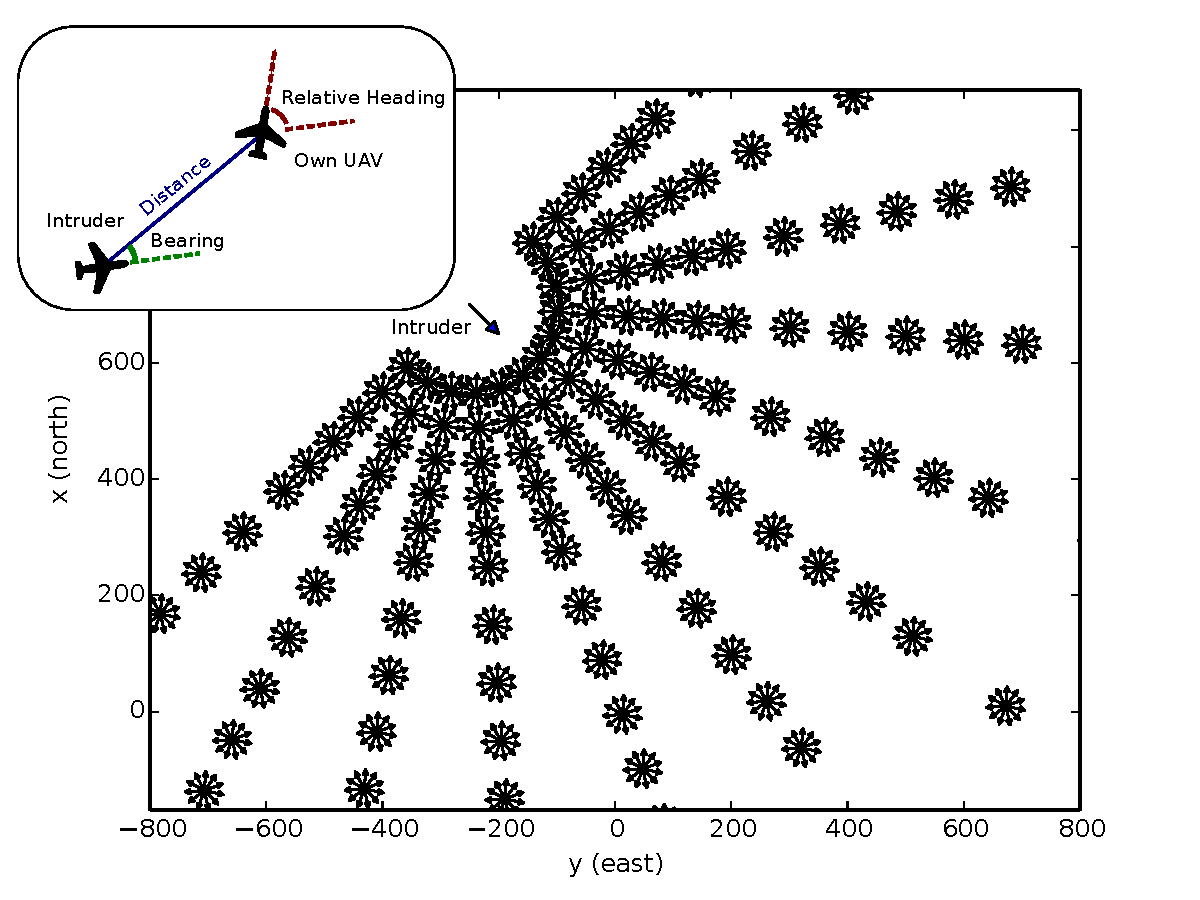
\includegraphics[width=0.8\textwidth]{media/intruder_grid_plus.pdf}
    \caption[Intruder interpolation grid]{Intruder interpolation grid for $\beta_\text{intruder}$, visualized when the intruder is located at (\SI{700}{m}, \SI{-250}{m}) at heading \num{135}. The top left inset shows the variables used. In the main plot, each of the small arrows represents a grid point. At each of the point locations, there are twelve small arrows radiating out. Each arrow represents a different UAV heading.}
    \label{fig:intrudergrid}
\end{figure}
\begin{figure}[p]
    \centering
    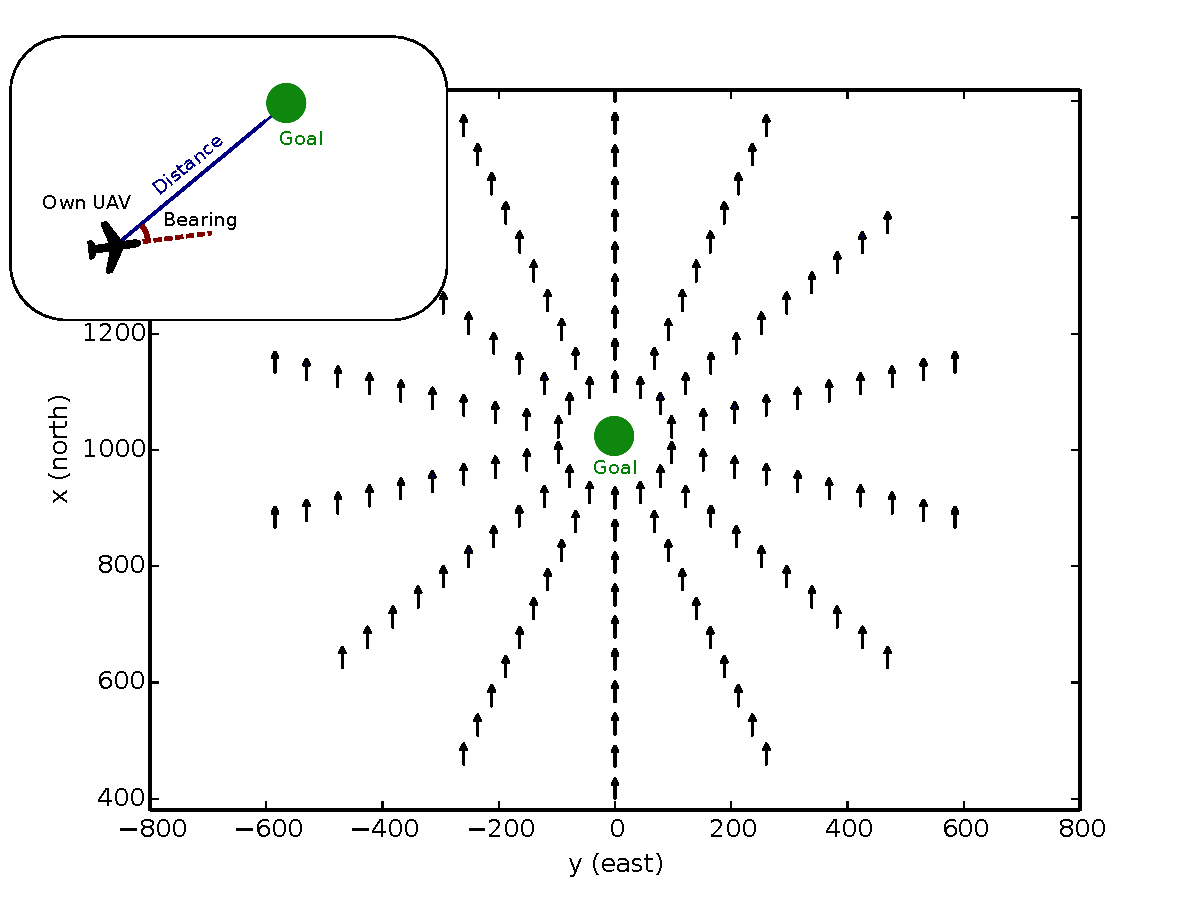
\includegraphics[width=0.8\textwidth]{media/goal_grid_plus.pdf}
    \caption[Goal interpolation grid]{Goal interpolation grid for $\beta_\text{goal}$ when the own UAV's heading is directly north. The grid takes advantage of symmetry in the bearing variable, so, for each arrow on the left side, there is an arrow on the right side that corresponds with the \emph{same} point in the grid.}
    \label{fig:goalgrid}
\end{figure}

Since the domain of $\beta_\text{intruder}$ is only three dimensional and the domain of $\beta_\text{goal}$ is only two dimensional, relatively fine interpolation grids can be used for value function approximation without requiring a prohibitively large number of features. The $\beta_\text{intruder}$ feature group consists of a NMAC indicator function and interpolation weights for a grid (\Cref{fig:intrudergrid}) with nodes at regularly spaced points along the following three variables: (1) the distance between the UAV and intruder, (2) the bearing from the intruder to the UAV, and (3) the relative heading between the vehicles. The $\beta_\text{goal}$ vector consists of a goal indicator function, the distance between the UAV and the goal, and interpolation weights for a grid (\Cref{fig:goalgrid}) with nodes regularly spaced along the distance between the UAV and the goal and the absolute value of the bearing to the goal from the UAV. The total number of features is $N_\beta = 1813$.


\section{Results} \label{sec:results}

This section presents results from numerical experiments that illustrate the effectiveness of the new approach. The experiments are designed to compare the four approaches discussed in \cref{sec:uavintro}: the ``static TRL'' approach, ``direct optimization'', and the new ``optimized TRL'' and ``trusted direct optimization'' approaches proposed in this chapter. The static TRL control law uses the TRL described in \cref{alg:trl} with a constant value for the separation distance (denoted with $\bar{D}$), while the other approaches use the approximate optimization procedure described in \cref{sec:approach}. The various parameters used in the numerical experiments are listed in \cref{tab:uparams}.

\subsection{Policies}

This section includes visualizations of two-dimensional ``slices'' of several UAV policies and their associated value functions. In each of the slices, the intruder is located at (\SI{700}{m}, \SI{-250}{m}) pointed at heading 135 as indicated by the arrow. The goal is at (\SI{1000}{m}, \num{0}). Each pixel on this image represents the value function or policy evaluated with the UAV at that position pointed directly north. As expected, for all approaches, there is a low value region in front of and to the south of the intruder and a high value region near the goal.

\Cref{fig:dovalue,fig:dopolicy} show the value function and policy for the directly optimized approach, and \cref{fig:tdovalue,fig:tdopolicy} show the same for the trusted directly optimized approach.
The policies for both approaches are similar, with regions in front of the intruder where sharp turns are commanded.
The trusted direct optimization policy is slightly more conservative with larger turn regions because of the restricted action space.

\begin{figure}[p]
    \centering
    \begin{subfigure}[t]{0.48\textwidth}
        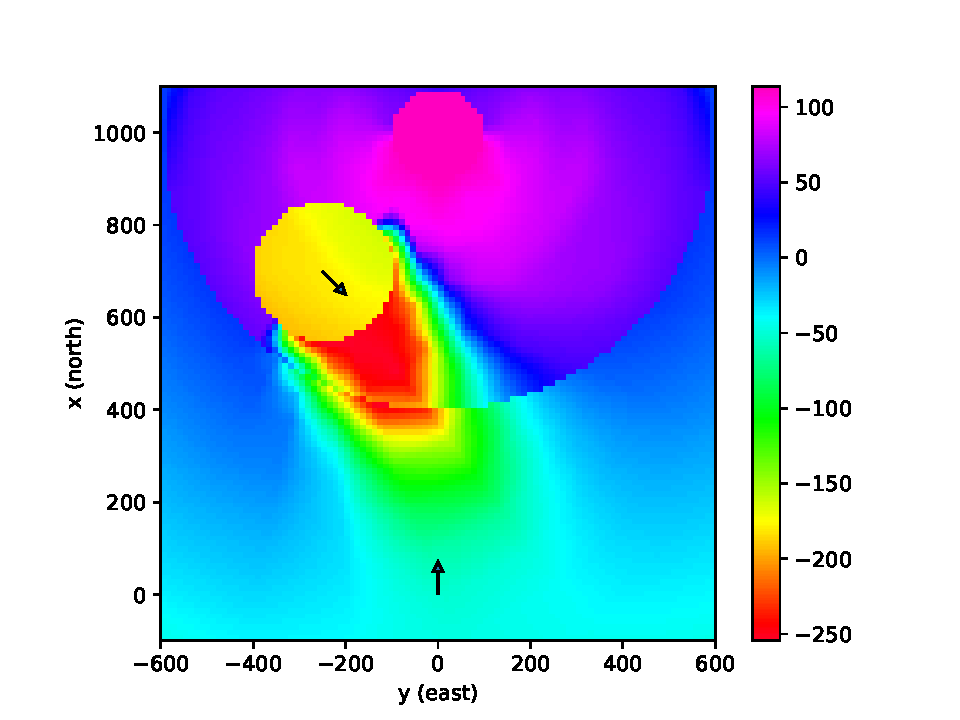
\includegraphics[width=\textwidth]{media/dovalue.pdf}
        \caption{Slice of the approximate optimal value function for direct optimization.}
        \label{fig:dovalue}
    \end{subfigure}
    \hfill
    \begin{subfigure}[t]{0.48\textwidth}
        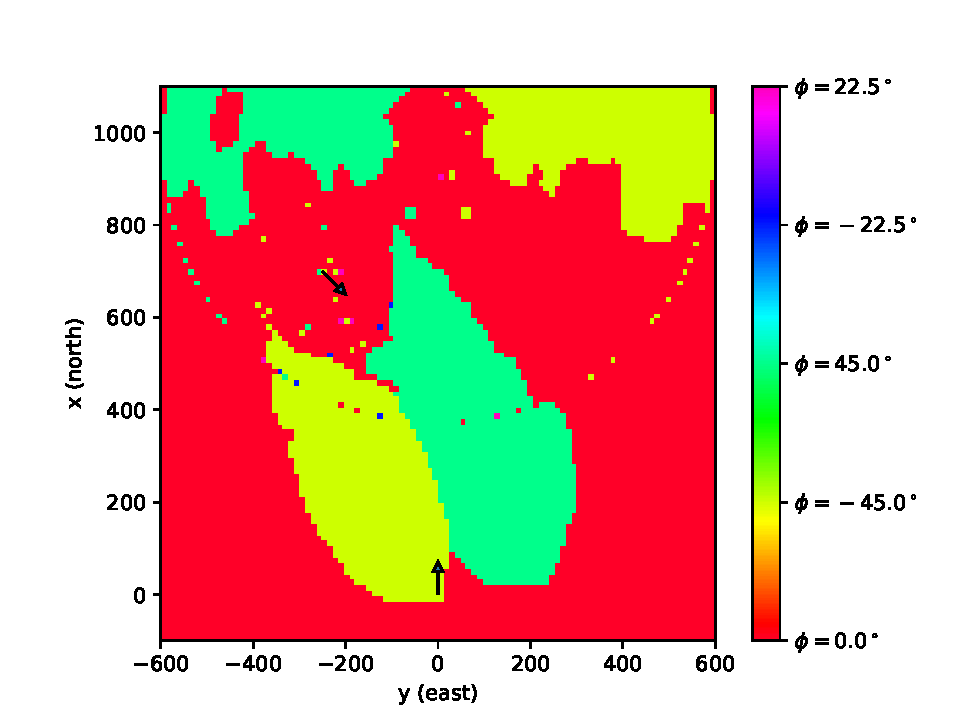
\includegraphics[width=\columnwidth]{media/dopolicy.pdf}
        \caption{Slice of the direct optimization policy.}
        \label{fig:dopolicy}
    \end{subfigure}

    \begin{subfigure}[t]{0.48\textwidth}
        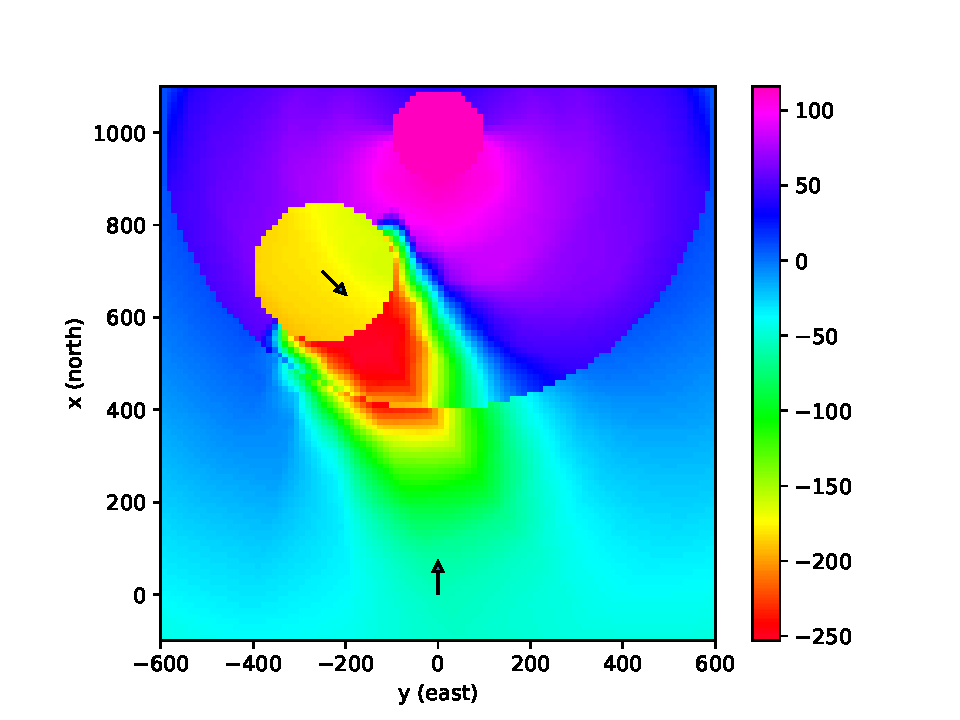
\includegraphics[width=\columnwidth]{media/tdovalue.pdf}
        \caption{Slice of the approximate optimal value function for trusted direct optimization.}
        \label{fig:tdovalue}
    \end{subfigure}
    \hfill
    \begin{subfigure}[t]{0.48\textwidth}
        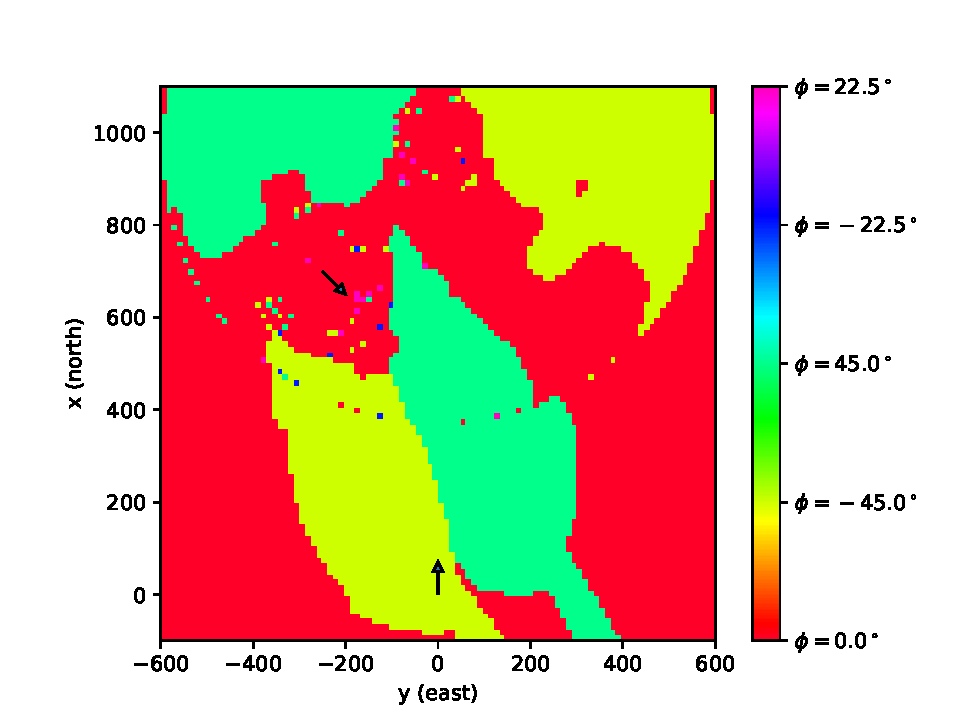
\includegraphics[width=\columnwidth]{media/tdopolicy.pdf}
        \caption{Slice of the trusted direct optimization policy.}
        \label{fig:tdopolicy}
    \end{subfigure}

    \begin{subfigure}[t]{0.48\textwidth}
        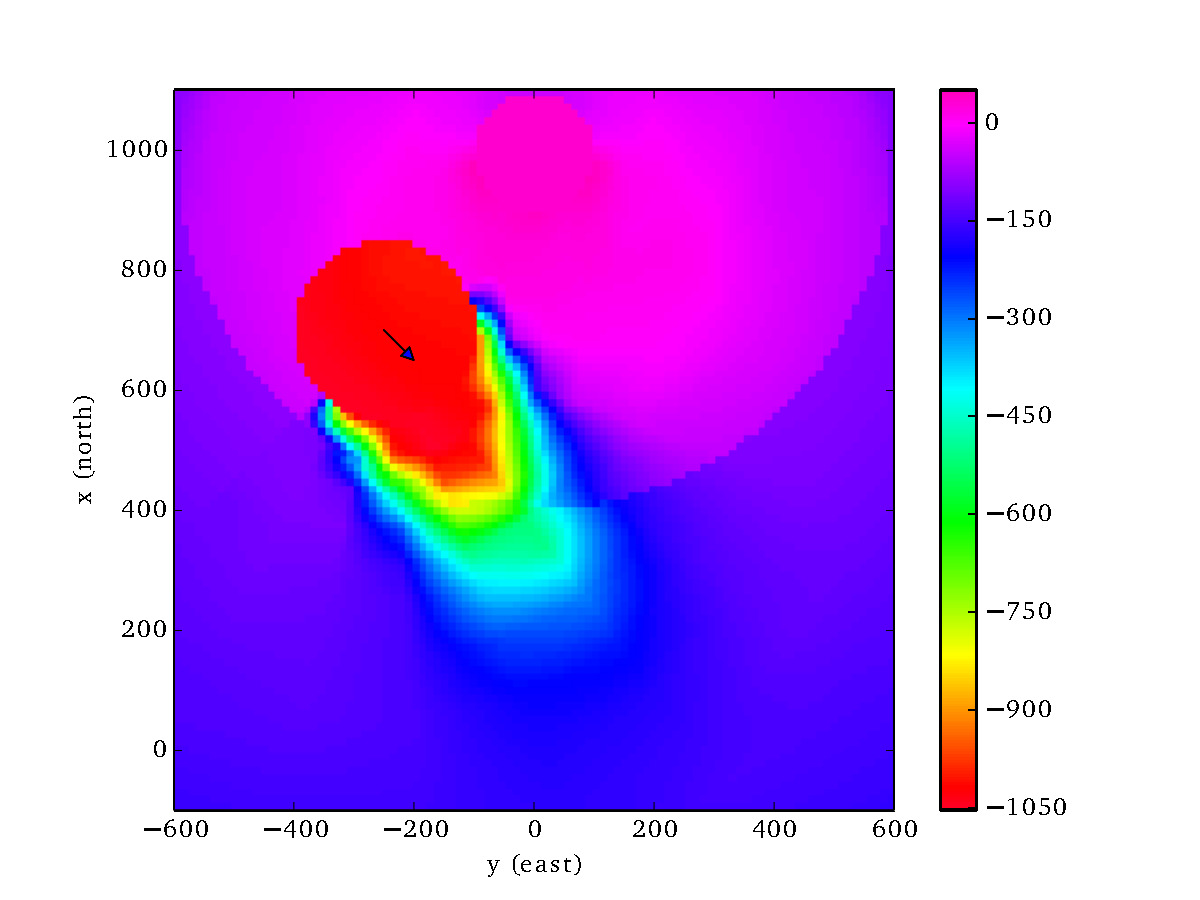
\includegraphics[width=\columnwidth]{media/value.pdf}
        \caption{Slice of the approximate optimal value function for the optimized TRL.} 
        \label{fig:trlvalue}
    \end{subfigure}
    \hfill
    \begin{subfigure}[t]{0.48\textwidth}
        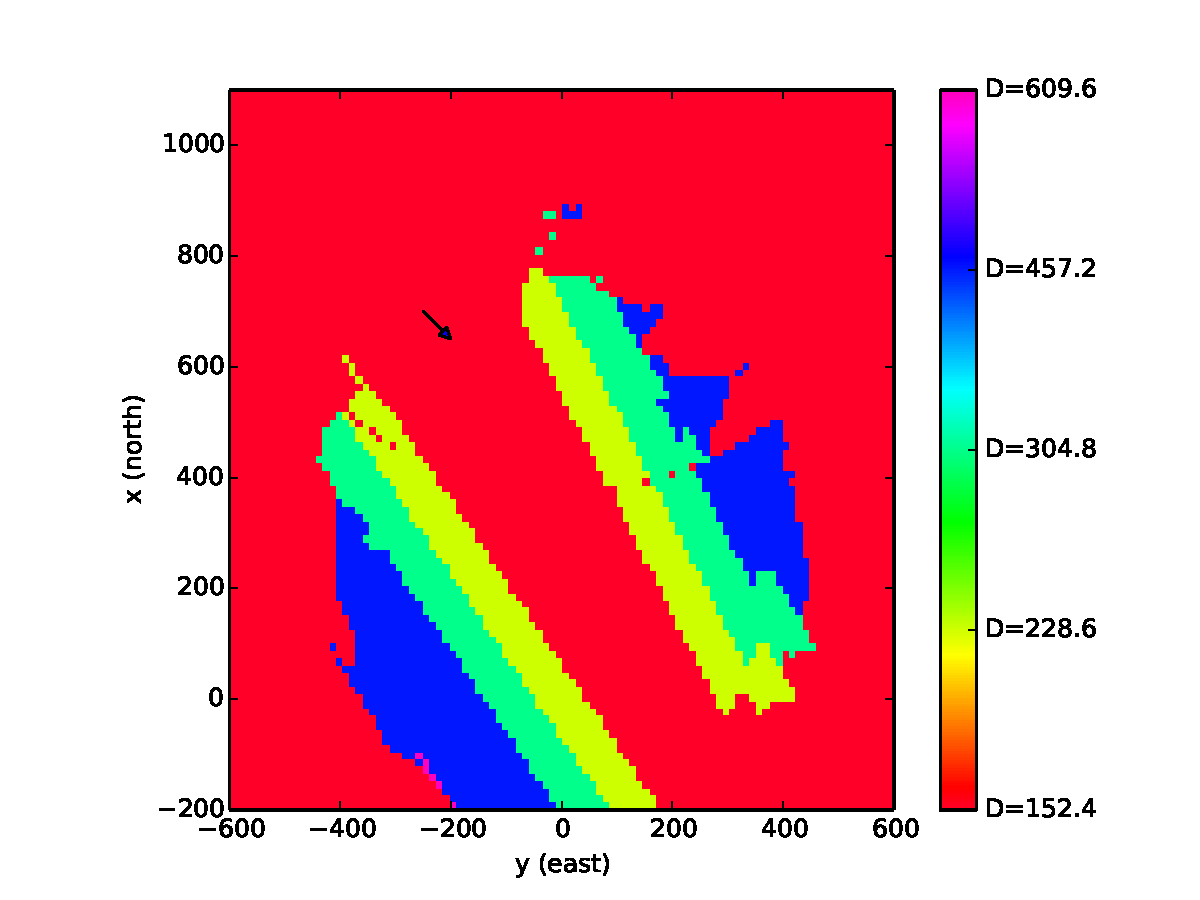
\includegraphics[width=\columnwidth]{media/policy.pdf}
        \caption{Slice of the optimized TRL policy.}
        \label{fig:trlpolicy}
    \end{subfigure}    
    \caption{UAV Collision avoidance policy visualizations}
\end{figure}



\Cref{fig:trlpolicy} shows the value function and policy for the optimized TRL approach. 
When multiple actions result in the same post decision state value, the least conservative action is chosen, so the policy yields the lowest value of $D$ ($\num{500} \si{ft} \approx \num{152.4} \si{m}$) on most of the state space. Because the own UAV is pointed north, the policy is conservative in a region in front of and to the south of the intruder. The band corresponding to small $D$ that stretches across the middle of the conservative region (from (\SI{700}{m},\SI{-250}{m}) to (\SI{-100}{m},\SI{200}{m})) is present because all values of $D$ result in the same post decision value.

\subsection{Numerical Performance Evaluation}

The control polices are evaluated by executing them in a large number of complete (from $t=0$ to the end state) encounter simulations. The same random numbers used to generate intruder noise were reused across all collision avoidance  strategies to ensure fairness of comparisons. In each of the simulations, the own UAV starts pointed north at position $(0,0)$ in a north-east coordinate system with the goal at $(1000\si{m},0)$.

The evaluation simulations use the same intruder random turn rate model with standard deviation $\sigma_{\dot{\psi}}$ that was used for value iteration. A robustness study using different models is not presented here, but previous research~\cite{MJK-JPC-PPR:10} suggests that this method will offer good performance when evaluated against both a range of noise parameters and structurally different models. The intruder initial position is randomly generated between \SI{800}{m} and \SI{1500}{m} from the center point of the encounter area at $(500\si{m},500\si{m})$ with an initial heading that is within \ang{135} of the direction from the initial position to the center point. 

The conservativeness of each control law is characterized by counting the number of deviations from the nominal path in \num{10000} simulations with initial conditions shown in \cref{fig:intruderics}.
Of these simulations, \num{1009} result in a NMAC if the UAV follows its nominal path, but for most a deviation would not be necessary to avoid the intruder.

The fraction of collisions avoided is estimated using a separate set of \num{10000} simulations. Each of these simulations has an initial condition in the same region described above, but initial conditions and noise trajectories are chosen by filtering random trials so that each of the simulations \emph{will result in a NMAC if the own UAV follows its nominal path}.

\begin{table}[tbp]
    \caption{Parameters for numerical experiments} \label{tab:uparams}
    \centering
    \begin{tabular}{p{0.6\columnwidth} l r}
        \toprule
        Description & Symbol & Value \\
        \midrule
        Own UAV speed & $\own{v}$ & \num{30} \si{m/s} \\
        Maximum own UAV bank angle & $\phi_\text{max}$ & \ang{45} \\
        Intruder speed & $\intr{v}$ & \num{60} \si{m/s} \\
        Intruder turn rate standard deviation & $\sigma_{\dot{\psi}}$ & \ang{10}\si{/s} \\
        Near mid air collision radius & $\dnmac$ & \num{500} \si{ft} \\
        Step cost & $c_\text{step}$ & \num{1} \\
        Reward for reaching goal & $r_\text{goal}$ & \num{100} \\
        Cost for deviation & $c_\text{dev}$ & \num{100} \\
        Step simulations for expectation estimate & $N_{EV}$ & \num{20} \\
        Single step simulations per round of value iteration (optimized TRL) & $N_\text{state}$ & \num{10000} \\
        Single step simulations per round of value iteration (directly optimized) & $N_\text{state}$ & \num{50000} \\
        Number of value iteration rounds & $N_{VI}$ & \num{35} \\
        Single step simulations for post decision value function extraction & $N_q$ & \num{50000} \\
        \bottomrule
    \end{tabular}
\end{table}

\begin{figure}[tbp]
    \centering
    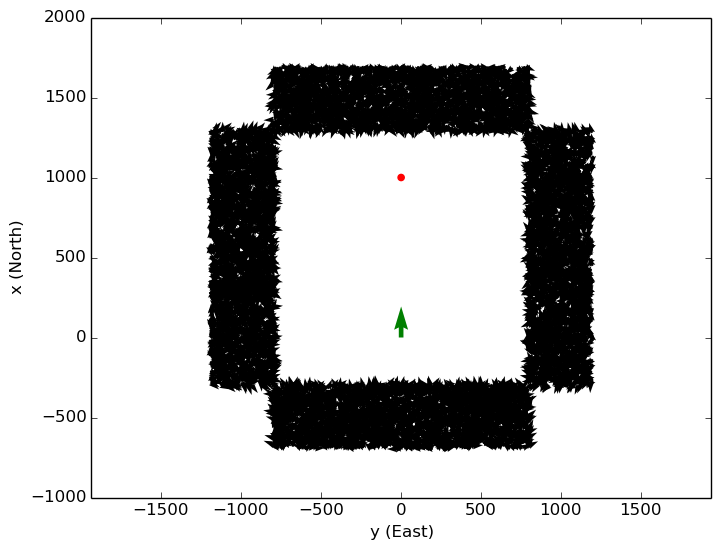
\includegraphics[width=0.8\columnwidth]{media/intruderics.png}
    \caption[Intruder initial conditions]{Intruder initial conditions for evaluation simulations. Each small black arrow is an intruder initial state. The large green arrow is the UAV's initial state. The red dot is the goal.}
    \label{fig:intruderics}
\end{figure}

\begin{figure}[tbp]
    \centering
    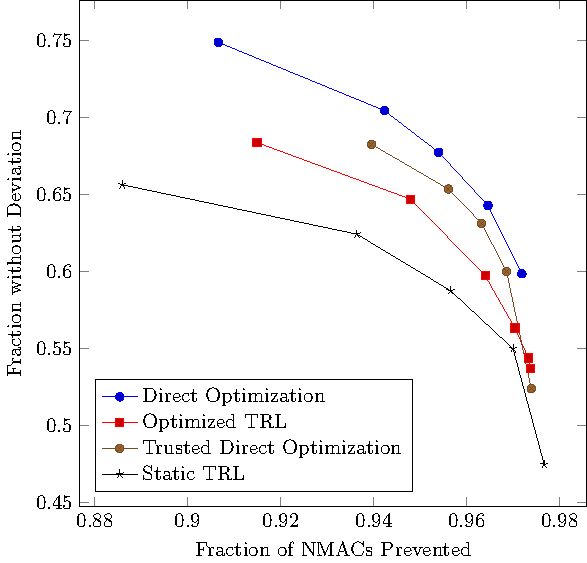
\includegraphics[width=0.7\columnwidth]{media/pareto.pdf}
    \caption[Policy performance comparison]{Policy performance comparison. The values of $\lambda$ used to generate the datapoints are \num{100}, \num{316}, \num{1000}, \num{3160}, \num{e4}, and \num{3.16e4} for the optimized TRL policy and \num{300}, \num{500}, \num{700}, \num{1000}, and \num{1500} for the directly optimized approach. The values of $\bar{D}$ for the static TRL policy are \SI{250}{m}, \SI{300}{m}, \SI{350}{m}, \SI{400}{m}, and \SI{500}{m}.}
       \label{fig:pareto}
\end{figure}

\Cref{fig:pareto} shows the Pareto optimal frontiers for the different control laws. Each curve is generated by using various values of $\lambda$ in the reward function of the MDP, or by using various static values of $\bar{D}$ in the static TRL case. It is clear that the optimization provides better performance than the static TRL. For example, if the desired fraction of NMACs prevented is $96\%$, interpolation between data points suggests that direct optimization will cause approximately $20\%$ fewer deviations than the static TRL policy. This difference may be interpreted as the \emph{price} if using trusted resolution logic rather than optimization.

Fortunately, both the optimized TRL and trusted direct optimization approaches offer ways to reduce this price.
Neither should be much more difficult to certify than the TRL because they are both based on the TRL.
In particular, neither will ever command an action that is deemed unsafe by the TRL. 
Thus, they provide the same level of trust as the TRL and thus reduce the price of trust.
In this case, trusted direct optimization is able to nearly close the gap between static TRL and direct optimization, while optimized TRL reduces the gap by about half, so trusted direct optimization would be the preferred approach.

The software used to simulate these experiments was written in the Julia programming language, and is freely available at \texttt{\small{https://github.com/zsunberg/UASEncounter}}.

\section{Discussion}

This chapter has explored using trusted resolution logic alongside approximate optimization to produce a high performance collision avoidance system for UAV that is also relatively easy to certify.
Due to flight performance and regulatory constraints, only horizontal maneuvers are considered when resolving potential collisions and the intruding aircraft is presumed to be unaware of the UAV.
This problem is formulated as a Markov decision process.
It is solved using an approximate value iteration approach.
This general approach is widely used~\cite{kochenderfer2015decision}, though problems of this size are still challenging to handle.
By choosing appropriate features and using a post-decision state, the method is made tractable for this problem.

% Using simple trusted resolution logic, where the UAV simply chooses the closest heading to the goal direction that will never pass within a specified distance $D$ of the intruder maintaining its current heading is an alternate approach.
Using simple trusted resolution logic that guarantees a separation distance $D$ if the intruder maintains its current heading is an alternate approach.
This approach has the advantage that it can be easily certified because, by construction, it will never command a heading that is considered dangerous.
However, when this TRL is compared to an approximate dynamic programming solution to the MDP, it is too conservative, causing unnecessary disruption to normal flight.
These tests demonstrate that there is a price that comes with certifiability and trustworthiness, and the performance gap between the approaches quantifies this price. Two alternative combinations of approximate dynamic programming and the TRL are considered as ways to reduce the price.

First, approximate dynamic programming is applied to dynamically choose $D$ within a certified range based on the encounter state.
Since every potential action is pre-certified, this approach retains the ease of certification of the TRL approach.
However, since this new action space is relatively limited, it only reduces the price by about half.

The second approach is to filter the original action space of turning maneuvers through the TRL so that the UAV may only take actions that will maintain $D$ separation based on the current state.
This approach should also be easy to certify, and it largely closes the performance gap, nearly eliminating the price of certifiability.

There are many potential extensions for this work.
First, the function approximation for the value iteration could be improved.
The feature-based approach used here worked well, but the selection of the features was mostly heuristically justified, and another more advanced and general approximation technique such as neural networks~\cite{goodfellow2016deep} may work better.
Most importantly, the uncertainty model should be improved.
The current model was not justified with data, and it is extremely unlikely that a Gaussian noise model reflects real intruder behavior.
It is much more plausible that the intruder has an operational intention unknown to the UAV which should be modeled as a hidden state in the problem.
It is not immediately clear how to solve the resulting POMDP offline, but a QMDP approach using the MDP solution found in this work may be adequate.
This concept of a hidden internal state governing the behavior of other agents is investigated in the next chapter, but in a different context: self-driving cars.

\chapter{The Value of Planning with the Internal State of Traffic Participants in Autonomous Freeway Driving}

\section{Human-Robot Interaction in Autonomous Driving}

\section{Freeway Driving POMDP}

\subsection{IDM-Mobil Driver Model}
\subsection{Parameter Correlation}
\subsection{Reward Function}

\section{Solution Approaches}

\section{Results}

\chapter{Online Algorithms for Continuous POMDPs} \label{chap:pomcpow}

The autonomous driving problem in the previous chapter illustrates that modeling partially observable internal states can have a significant effect on performance.
POMDPs based on real world problems, such as the one considered in~\cref{chap:multilane}, often have continuous state, action, and observation spaces.
Although the research surveyed in \cref{sec:solutions} has yielded effective solution techniques for many classes of POMDPs, there remains a need for simple, general purpose online solvers that can handle continuous spaces, especially continuous observation spaces.
This chapter takes some important steps toward addressing that need.

POMCP and other online methods can easily accomodate continuous state spaces without any modification \cite{goldhoorn2014continuous}.
However, there has been less progress on problems with continuous observation spaces.
This chapter presents two similar algorithms which address the challenge of solving POMDPs with continuous state, action, and observation spaces.
The first is based on POMCP and is called partially observable Monte Carlo planning with observation widening (POMCPOW). 
The second solves the belief-space MDP and is called particle filter trees with double progressive widening (PFT-DPW).

\section{Background}

\begin{figure}[htb]
\begin{center}
    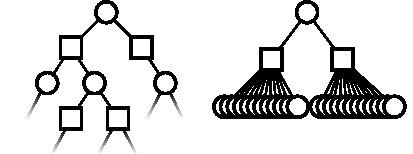
\includegraphics[width=0.9\columnwidth]{media/continuous_tree.pdf}
\end{center}
\caption[POMCP tree on a continuous observation space]{POMCP tree for a discrete POMDP (left), and for a POMDP with a continuous observation space (right). Because the observation space is continuous, each simulation creates a new observation node and the tree cannot extend deeper.}
\label{fig:ctree}
\end{figure}

There are two challenges that make tree search difficult in continuous spaces.
The first is that, since the probability of sampling the same real number twice from a continuous random variable is zero, the width of the planning trees explodes on the first step, causing them to be too shallow to be useful (see \cref{fig:ctree}).
POMCPOW and PFT-DPW resolve this issue with a technique called double progressive widening (DPW) \cite{couetoux2011double}. 
The second issue is that, even when DPW is applied, the belief representations used by current solvers collapse to a single state particle, resulting in overconfidence.
As a consequence, the solutions obtained resemble QMDP policies, and there is no incentive for information gathering.
POMCPOW and PFT-DPW overcome this issue by using the observation model to weight the particles used to represent beliefs.

A small amount of previous research has sought online solutions to continuous POMDPs.
ABT has been extended to use generalized pattern search for selecting locally optimal continuous actions, an approach which is especially effective in problems where high precision is important \cite{seiler2015online}.
Continuous observation Monte Carlo tree search (COMCTS) constructs observation classification trees to automatically partition the observation space in a POMCP-like approach, however it did not perform much better than a Monte Carlo rollout approach in experiments \cite{pas2012simulation}.

\section{Algorithms}

This section presents and discusses several methods for handling continuous POMDPs.
First, it presents three new MCTS-DPW-based algorithms.
The first of these is POMCP-DPW.
\Cref{thm:qmdp} shows that this algorithm is suboptimal in some cases.
The second algorithm is PFT-DPW, a straightforward application of MCTS-DPW to the belief MDP with particle filters to approximate belief updates.
The third algorithm is POMCPOW, which fixes the problems noted about POMCP-DPW and successfully extends POMCP to problems with continuous observation spaces.
These three algorithms are followed by brief discussion about the discretization alternative to these algorithms and the additional observation distribution requirement of POMCPOW and PFT-DPW.

The three new algorithms in this chapter share a common structure.
For all algorithms, the entry point for the decision making process is the \textproc{Plan} procedure, which takes the current belief, $b$, as an input (\textproc{Plan} differs slightly for PFT-DPW in \cref{alg:pft}).
The algorithms also share the same \textproc{ActionProgWiden} function to control progressive widening of the action space.
These components are listed in Listing \ref{alg:common}.
The difference between the algorithms is in the \textproc{Simulate} function.

The following variables are used in the listings and text:
$h$ represents a history $(b, a_1, o_1, \dots a_k, o_k)$, and $ha$ and $hao$ are shorthand for histories with $a$ and $(a,o)$ appended to the end, respectively;
$d$ is the depth to explore, with $d_\text{max}$ the maximum depth;
$C$ is a list of the children of a node (along with the reward in the case of PFT-DPW);
$N$ is a count of the number of visits; and $M$ is a count of the number of times that a history has been generated by the model.
The list of states associated with a node is denoted $B$, and $W$ is a list of weights corresponding to those states.
Finally, $Q(ha)$ is an estimate of the value of taking action $a$ after observing history $h$.
$C$, $N$, $M$, $B$, $W$, and $Q$ are all implicitly initialized to \num{0} or $\emptyset$.
The \textproc{Rollout} procedure, runs a simulation with a default rollout policy, which can be based on the history or fully observed state, for $d$ steps and returns the discounted reward.

% TODO algorithm vs listing numbering
\begin{algorithm}[htbp]
    \floatname{algorithm}{Listing}
    \caption{Common procedures} \label{alg:common}
    \begin{algorithmic}[1]
        \Procedure{Plan}{$b$}
            \For{$i \in 1:n$}
                \State $s \gets \text{sample from }b$
                \State $\Call{Simulate}{s, b, d_\text{max}}$
            \EndFor
            \State $\textbf{return } \underset{a}{\argmax}\, Q(ba)$
        \EndProcedure

        \Procedure {ActionProgWiden}{$h$}
            \If{$|C(h)| \leq k_a N(h)^{\alpha_a}$}
                \State $a \gets \Call{NextAction}{h}$
                \State $C(h) \gets C(h) \cup \{a\}$
            \EndIf
            \State $\textbf{return } \underset{a \in C(h)}{\argmax}\, Q(ha) + c \sqrt{\frac{\log N(h)}{N(ha)}}$
        \EndProcedure

    \end{algorithmic}
\end{algorithm}


\subsection{POMCP-DPW}

The first algorithm that we consider is POMCP with double progressive widening (POMCP-DPW).
In this algorithm, listed in \cref{alg:pomcpdpw}, the number of new children sampled from any node in the tree is limited by DPW using the parameters $k_a$, $\alpha_a$, $k_o$, and $\alpha_o$.
In the case where the simulated observation is rejected (line~\ref{lin:notnew}), the tree search is continued with an observation selected in proportion to the number of times, $M$, it has been previously simulated (line~\ref{lin:selecto}) and a state is sampled from the associated belief (line~\ref{lin:samples}).

\setcounter{algorithm}{0}
\begin{algorithm}[htbp]
    \caption{POMCP-DPW} \label{alg:pomcpdpw}
    \begin{algorithmic}[1]
        \Procedure {Simulate}{$s$, $h$, $d$}        
            \If{$d = 0$}
                \State \textbf{return} $0$
            \EndIf
            \State $a \gets \Call{ActionProgWiden}{h}$
            \If{$|C(ha)| \leq k_o N(ha)^{\alpha_o}$}
                \State $s',o,r \gets G(s,a)$
                \State $C(ha) \gets C(ha) \cup \{o\}$
                \State $M(hao) \gets M(hao) + 1$
                \State $\text{append } s' \text{ to } B(hao)$ \label{lin:insertion}
                \If{$M(hao) = 1$}
                    \State $total \gets r + \gamma \Call{Rollout}{s', hao, d-1}$
                \Else
                    \State $total \gets r + \gamma \Call{Simulate}{s', hao, d-1}$
                \EndIf
            \Else \label{lin:notnew}
                \State $o \gets \text{select } o \in C(ha) \text{ w.p. } \frac{M(hao)}{\sum_{o} M(hao)}$ \label{lin:selecto}
                \State $s' \gets \text{select } s' \in B(hao) \text{ w.p. } \frac{1}{|B(hao)|}$ \label{lin:samples}
                \State $r \gets R(s,a,s')$
                \State $total \gets r + \gamma \Call{Simulate}{s', hao, d-1}$
            \EndIf
            \State $N(h) \gets N(h)+1$
            \State $N(ha) \gets N(ha)+1$
            \State $Q(ha) \gets Q(ha) + \frac{total - Q(ha)}{N(ha)}$
            \State \textbf{return} $total$
        \EndProcedure
    \end{algorithmic}
\end{algorithm}

This algorithm obtained remarkably good solutions for a very large autonomous freeway driving POMDP with multiple vehicles (up to 40 continuous fully observable state dimensions and 72 continuous correlated partially observable state dimensions) \cite{sunberg2017value}.
To our knowledge, that is the first work applying progressive widening to POMCP, and it does not contain a detailed description of the algorithm or any theoretical or experimental analysis other than the driving application.

This algorithm may converge to the optimal solution for POMDPs with discrete observation spaces; however, on continuous observation spaces, POMCP-DPW is suboptimal.
In particular, it finds a QMDP policy (see \cref{sec:qmdp}).
In fact, for a modified version of POMCP-DPW, it is easy to prove analytically that it will converge to such a policy.
This is expressed formally in Theorem~\ref{thm:qmdp} below.
A complete description of the modified algorithm and problem requirements including the definitions of polynomial exploration, the regularity hypothesis for the problem, and exponentially sure convergence are given in \cref{sec:proof}.

\begin{definition}[QMDP value]
    Let $Q_\text{MDP}(s,a)$ be the optimal state-action value function assuming full observability starting by taking action $a$ in state $s$. The \emph{QMDP value} at belief $b$, $Q_\text{MDP}(b,a)$, is the expected value of $Q_\text{MDP}(s,a)$ when $s$ is distributed according to $b$.
\end{definition}

% \begin{theorem}[Modified POMCP-DPW convergence to QMDP] \label{thm:qmdp}
\begin{restatable}[Modified POMCP-DPW convergence to QMDP]{theorem}{qmdp}
    \label{thm:qmdp}
If a bounded-horizon POMDP meets the following conditions: 1) the state and observation spaces are continuous with a finite observation probability density function, and 2) the regularity hypothesis is met, then modified POMCP-DPW will produce a value function estimate, $\hat{Q}$, that converges to the QMDP value for the problem.
Specifically, there exists a constant $C>0$, such that after $n$ iterations,
\begin{equation*}
    \left| \hat{Q}(b,a) - Q_\text{MDP}(b,a) \right| \leq \frac{C}{n^{1/(10d_{\max}-7)}}
\end{equation*}
exponentially surely in $n$, for every action $a$.
\end{restatable}
% \end{theorem}

A proof of this theorem that leverages work by \citet{auger2013continuous} is given in \cref{sec:proof}, but I will provide a brief justification here.
The key is that belief nodes will contain only a single state particle (see \cref{fig:treecomp}).
This is because, since the observation space is continuous with a finite density function, the generative model will (with probability one) produce a unique observation $o$ each time it is queried.
Thus, for every generated history $h$, only one state will ever be inserted into $B(h)$ (line~\ref{lin:insertion}, \cref{alg:pomcpdpw}), and therefore $h$ is merely an alias for that state. 
Since each belief node corresponds to a state, the solver is actually solving the fully observable MDP at every node except the root node, leading to a QMDP solution.

As a result of \cref{thm:qmdp}, the action chosen by modified POMCP-DPW will match a QMDP policy (a policy of actions that maximize the QMDP value) with high precision exponentially surely (see Corollary 1 of \citet{auger2013continuous}).
For many problems this is a very useful solution,\footnote{Indeed, a useful online QMDP tree search algorithm could be created by deliberately constructing a tree with a single root belief node and fully observable state nodes below it.} but since it neglects the value of information, a QMDP policy is suboptimal for problems where information gathering is important \cite{littman1995learning,kochenderfer2015decision}.
% This phenomenon is demonstrated in simulation in \cref{sec:lightdark}.

Although \cref{thm:qmdp} is only theoretically applicable to the modified version of POMCP-DPW, it helps explain the behavior of other solvers.
Modified POMCP-DPW, POMCP-DPW, DESPOT, and ABT all share the characteristic that a belief node can only contain two states if they generated exactly the same observation.
Since this is an event with zero probability for a continuous observation space, these solvers exhibit suboptimal, often QMDP-like, behavior.
The experiments in \cref{sec:discgran} show this for POMCP-DPW and DESPOT, and this is presumably the case for ABT as well.


\begin{figure}[htpb]
    \centering
    \begin{subfigure}[b]{0.45\columnwidth}
        \centering
        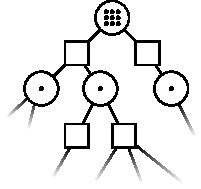
\includegraphics[width=\textwidth]{media/dpw_tree.pdf}
        \caption{POMCP-DPW Tree}
    \end{subfigure}
    \begin{subfigure}[b]{0.45\columnwidth}
        \centering
        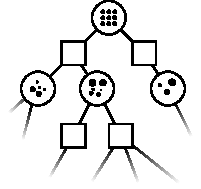
\includegraphics[width=\textwidth]{media/pomcpow_tree.pdf}
        \caption{POMCPOW Tree}
    \end{subfigure}
    \caption[POMCP-DPW and POMCPOW tree structure comparison]{Tree structure comparison. Each square is an action node, and each unfilled circle is an observation node. Each black dot corresponds to a state particle with the size representing its weight. In continuous observation spaces, the beliefs in a POMCP-DPW tree degenerate to a single particle, while POMCPOW maintains weighted particle mixture beliefs.}
    \label{fig:treecomp}
\end{figure}

\subsection{PFT-DPW}

Another algorithm that one might consider for solving continuous POMDPs online is MCTS-DPW on the equivalent belief MDP.
Since the Bayesian belief update is usually computationally intractable, a particle filter is used.
This new approach will be referred to as particle filter trees with double progressive widening (PFT-DPW).
It is shown in \cref{alg:pft}, where $G_\text{PF($m$)}(b,a)$ is a particle filter belief update performed with a simulated observation and $m$ state particles which approximates the belief MDP generative model.
The authors are not aware of any mention of this algorithm in prior literature, but it is very likely that MCTS with particle filters has been used before without double progressive widening under another name.

PFT-DPW is fundamentally different from POMCP and POMCPOW because it relies on simulating approximate belief trajectories instead of state trajectories.
This distinction also allows it to be applied to problems where the reward is a function of the belief rather than the state such as pure information-gathering problems \cite{dressel2017efficient,araya2010pomdp}.

The primary shortcoming of this algorithm is that the number of particles in the filter, $m$, must be chosen a-priori and is static throughout the tree.
Each time a new belief node is created, an $\mathcal{O}(m)$ particle filter update is performed.
If $m$ is too small, the beliefs may miss important states, but if $m$ is too large, constructing the tree is expensive.
Fortunately, the experiments in \cref{sec:experiments} show that it is often easy to choose $m$ in practice; for all the problems studied here, a value of $m=20$ resulted in good performance.


\begin{algorithm}[htbp]
    \caption{PFT-DPW} \label{alg:pft}
    \begin{algorithmic}[1]
        \Procedure{Plan}{$b$}
            \For{$i \in 1:n$}
                \State $\Call{Simulate}{b, d_\text{max}}$
            \EndFor
            \State $\textbf{return } \underset{a}{\argmax}\, Q(ba)$
        \EndProcedure
        \Procedure {Simulate}{$b$, $d$}        
            \If{$d = 0$}
                \State \textbf{return} $0$
            \EndIf
            \State $a \gets \Call{ActionProgWiden}{b}$
            \If{$|C(ba)| \leq k_o N(ba)^{\alpha_o}$}
                \State $b',r \gets G_\text{PF($m$)}(b,a)$
                \State $C(ba) \gets C(ba) \cup \{(b',r)\}$
                \State $total \gets r + \gamma \Call{Rollout}{b', d-1}$
            \Else
                \State $b', r \gets \text{sample uniformly from } C(ba)$
                \State $total \gets r + \gamma \Call{Simulate}{b', d-1}$
            \EndIf
            \State $N(b) \gets N(b)+1$
            \State $N(ba) \gets N(ba)+1$
            \State $Q(ba) \gets Q(ba) + \frac{total - Q(ba)}{N(ba)}$
            \State \textbf{return} $total$
        \EndProcedure
    \end{algorithmic}
\end{algorithm}

\subsection{POMCPOW} \label{sec:pomcpow}

\begin{algorithm}[htbp]
    \caption{POMCPOW} \label{alg:pomcpow}
    \begin{algorithmic}[1]
        \Procedure {Simulate}{$s$, $h$, $d$}        
            \If{$d = 0$}
                \State \textbf{return} $0$
            \EndIf
            \State $a \gets \Call{ActionProgWiden}{h}$
            \State $s',o,r \gets G(s,a)$
            \If{$|C(ha)| \leq k_o N(ha)^{\alpha_o}$}
                \State $M(hao) \gets M(hao) + 1$
            \Else
                \State $o \gets \text{select } o \in C(ha) \text{ w.p. } \frac{M(hao)}{\sum_{o} M(hao)}$
            \EndIf
            \State $\text{append } s' \text{ to } B(hao)$ \label{lin:insert}
            \State $\text{append } \odist(o \mid s, a, s') \text{ to } W(hao)$ \label{lin:weight}
            \If{$o \notin C(ha)$} \Comment{new node}
                \State $C(ha) \gets C(ha) \cup \{o\}$
                \State $total \gets r + \gamma \Call{Rollout}{s', hao, d-1}$
            \Else
                \State $s' \gets \text{select } B(hao)[i] \text{ w.p. } \frac{W(hao)[i]}{\sum_{j=1}^m W(hao)[j]}$ \label{lin:sample}
                \State $r \gets R(s,a,s')$
                \State $total \gets r + \gamma \Call{Simulate}{s', hao, d-1}$
            \EndIf
            \State $N(h) \gets N(h)+1$
            \State $N(ha) \gets N(ha)+1$
            \State $Q(ha) \gets Q(ha) + \frac{total - Q(ha)}{N(ha)}$
            \State \textbf{return} $total$
        \EndProcedure
    \end{algorithmic}
\end{algorithm}


In order to address the suboptimality of POMCP-DPW, we now propose a new algorithm, POMCPOW, shown in \cref{alg:pomcpow}.
In this algorithm, the belief updates are weighted, but they also expand gradually as more simulations are added.
Furthermore, since the richness of the belief representation is related to the number of times the node is visited, beliefs that are more likely to be reached by the optimal policy have more particles.
At each step, the simulated state is inserted into the weighted particle collection that represents the belief (line~\ref{lin:insert}), and a new state is sampled from that belief (line~\ref{lin:sample}).
A simple illustration of the tree is shown in \Cref{fig:treecomp} to contrast with a POMCP-DPW tree.
Because the resampling in line~\ref{lin:sample} can be efficiently implemented with binary search, the computational complexity is $\mathcal{O}(n d \log(n))$.

\subsection{Discretization} \label{sec:discretization}

Discretization is perhaps the most straightforward way to deal with continuous observation spaces.
In this approach, the continuous observation space is simply divided into small discrete regions and solved as a discrete POMDP using conventional methods.
The results in \cref{tab:experiments} show that this approach is only sometimes effective.

\subsection{Observation Distribution Requirement}

It is important to note that, while POMCP, POMCP-DPW, and DESPOT only require a generative model of the problem,  both POMCPOW and PFT-DPW require a way to query the relative likelihood of different observations ($\odist$ in line~\ref{lin:weight}).
One may object that this will limit the application of POMCPOW to a small class of POMDPs, but we think it will be an effective tool in practice for two reasons.

First, this requirement is no more stringent than the requirement for a standard importance resampling particle filter, and such filters are used widely, at least in the field of robotics that the authors are most familiar with. 
Moreover, if the observation model is complex, an approximate model may be sufficient.

Second, given the implications of \cref{thm:qmdp}, it is difficult to imagine a tree-based decision-making algorithm or a robust belief updater that does not require some way of measuring whether a state belongs to a belief or history.
The observation model is a straightforward and standard way of specifying such a measure.
Finally, in practice, except for the simplest of problems, using POMCP or DESPOT to repeatedly observe and act in an environment already requires more than just a generative model.
For example, the authors of the original paper describing POMCP~\cite{silver2010pomcp} use heuristic particle reinvigoration in lieu of an observation model and importance sampling.

\section{Experiments} \label{sec:experiments}

Numerical simulation experiments were conducted to evaluate the performance of POMCPOW and PFT-DPW compared to other solvers.
The open source code for the experiments is built on the POMDPs.jl framework (\cref{chap:pomdpsjl}) and is hosted at \url{https://github.com/zsunberg/ContinuousPOMDPTreeSearchExperiments.jl}.
In all experiments, the solvers were limited to \SI{1}{second} of computation time per step. Belief updates were accomplished with a particle filter independent of the planner, and no part of the tree was saved for re-use on subsequent steps.
Hyperparameter values are shown in \cref{sec:hyper}.

\begin{sidewaystable}
    {
        \caption{Experimental Results} \label{tab:experiments}

        \begin{tabularx}{\linewidth}{lXrlXrlXrl}
\toprule
& & Laser Tag \makebox[0pt][l]{(D, D, D)} & & & Light Dark \makebox[0pt][l]{(D, D, C)} & & & Sub Hunt \makebox[0pt][l]{(D, D, C)} & \\
\midrule
POMCPOW & & \result{-10.3}{0.2}{81}{0.81} & & \result{56.1}{0.6}{76}{0.76} & & \result{69.2}{1.3}{87}{0.87} \\
PFT-DPW & & \result{-11.1}{0.2}{74}{0.74} & & \result{57.2}{0.5}{77}{0.77} & & \result{77.4}{1.1}{97}{0.97} \\
QMDP & & \result{-10.5}{0.2}{79}{0.79} & & \result{-6.4}{1.0}{14}{0.14} & & \result{28.0}{1.3}{35}{0.35} \\
POMCP-DPW & & \result{-10.6}{0.2}{78}{0.78} & & \result{-7.3}{1.0}{13}{0.13} & & \result{28.3}{1.3}{35}{0.35} \\
DESPOT & & \result{-8.9}{0.2}{92}{0.92} & & \result{-6.8}{1.0}{13}{0.13} & & \result{26.8}{1.3}{34}{0.34} \\
POMCP\textsuperscript{D} & & \result{-14.1}{0.2}{49}{0.49} & & \result{61.1}{0.4}{81}{0.81} & & \result{28.0}{1.3}{35}{0.35} \\
DESPOT\textsuperscript{D} & & \noresult{} & & \result{54.2}{1.1}{74}{0.74} & & \result{27.4}{1.3}{34}{0.34} \\

\midrule
& & VDP Tag \makebox[0pt][l]{(C, C, C)} & & & Multilane \makebox[0pt][l]{(C, D, C)} & \\
\midrule
POMCPOW & & \result{29.3}{0.8}{95}{0.95} & & \result{30.9}{0.9}{70}{0.70} \\
PFT-DPW & & \result{27.2}{0.8}{88}{0.88} & & \result{21.4}{0.9}{38}{0.38} \\
QMDP & & \noresult{} & & \noresult{} \\
POMCP-DPW & & \result{16.4}{1.0}{53}{0.53} & & \result{29.6}{0.9}{65}{0.65} \\
DESPOT & & \noresult{} & & \result{36.0}{0.8}{87}{0.87} \\
POMCP\textsuperscript{D} & & \result{14.7}{0.9}{47}{0.47} & & \noresult{} \\
DESPOT\textsuperscript{D} & & \result{14.3}{1.0}{46}{0.46} & & \noresult{} \\

\bottomrule
\end{tabularx}


    }
    \vspace{5mm}
    \footnotesize{The three C or D characters after the solver indicate whether the state, action, and observation spaces are continuous or discrete, respectively. For continuous problems, solvers with a superscript D were run on a version of the problem with discretized action and observation spaces, but they interacted with continuous simulations of the problem.}
\end{sidewaystable}

\subsection{Laser Tag}

The Laser Tag benchmark (\cref{fig:lasertag}) is taken directly from the work of \citet{somani2013despot} and included for the sake of calibration. A complete description is given in that work. DESPOT outperforms the other methods in this test. The score for DESPOT differs slightly from that reported by \citet{somani2013despot} likely because of bounds implementation differences.
POMCP performs much better than reported by \citet{somani2013despot} because this implementation uses a state-based rollout policy.

\begin{figure}[htpb]
    \centering
    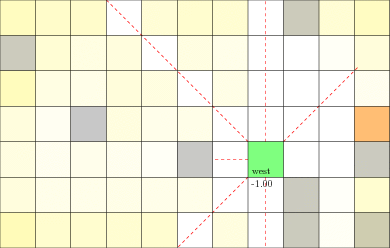
\includegraphics[width=0.6\linewidth]{media/lasertag.png}
    \caption[Laser Tag benchmark]{Laser Tag benchmark. The green square is the robot; the orange square is the target. The varying shades of yellow show the belief about the position of the target. The red dashed lines represent the laser sensors.}
    \label{fig:lasertag}
\end{figure}

\subsection{Light Dark}

In the Light Dark domain, the state is an integer between $-60$ and $60$, and the agent can choose how to move deterministically ($s' = s+a$) from the action space $\mathcal{A}=\{-10, -1, 0, 1, 10\}$. 
The goal is to reach the origin and take an action there.
If action $0$ is taken at the origin, a reward of $100$ is given and the problem terminates; If action $0$ is taken at another location, a penalty of $-100$ is given.
There is a cost of $-1$ at each step before termination.
The agent receives a more accurate observation in the ``light'' region around $s=10$.
Specifically, observations are continuous ($\ospace=\reals$) and normally distributed with standard deviation $\sigma=|s-10|$.

\Cref{tab:experiments} shows the mean reward from $1000$ simulations for each solver, and \cref{fig:ld} shows an example experiment.
The optimal strategy involves moving toward the light region and localizing before proceeding to the origin. 
QMDP and solvers predicted to behave like QMDP attempt to move directly to the origin, while POMCPOW and PFT-DPW perform better.
In this one-dimensional case, discretization allows POMCP to outperform all other methods and DESPOT to perform well, but in subsequent problems where the observation space has more dimensions, discretization does not provide the same performance improvement (see \cref{sec:discretization}).

\begin{figure}[htb]
    \centering
    % \input{ld_fig.pgf}
    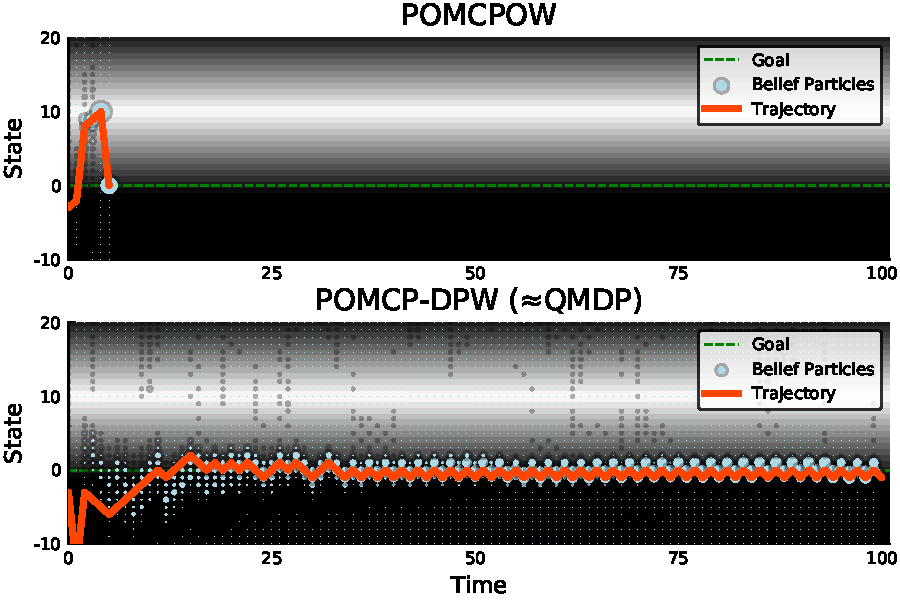
\includegraphics[width=0.6\columnwidth]{media/ld_fig.pdf}
    \caption[Light Dark problem]{Example trajectories in the Light Dark domain. POMCPOW travels to the light region and accurately localizes before moving to the goal. POMCP-DPW displays QMDP-like behavior: it is unable to localize well enough to take action \num{0} with confidence. The belief particles far away from \num{0} in the POMCP-DPW plot are due to particle reinvigoration that makes the filter more robust.}
    \label{fig:ld}
\end{figure}

\subsection{Sub Hunt}

In the Sub Hunt domain, the agent is a submarine attempting to track and destroy an enemy sub.
The state and action spaces are discrete so that QMDP can be used to solve the problem for comparison.
The agent and the target each occupy a cell of a 20 by 20 grid. The target is either aware or unaware of the agent and seeks to reach a particular edge of the grid unknown to the agent ($\mathcal{S} = \{1,..,20\}^4 \times \{\text{aware}, \text{unaware}\} \times \{N,S,E,W\}$).
The target stochastically moves either two steps towards the goal or one step forward and one to the side.
The agent has six actions, move three steps north, south, east, or west, engage the other submarine, or ping with active sonar.
If the agent chooses to engage and the target is unaware and within a range of 2, a hit with reward 100 is scored; The problem ends when a hit is scored or the target reaches its goal edge.

An observation consists of 8 sonar returns ($\ospace = \reals^8$) at equally-spaced angles that give a normally distributed estimate ($\sigma=0.5$) of the range to the target if the target is within that beam and a measurement with higher variance if it is not.
The range of the sensors depends on whether the agent decides to use active sonar.
If the agent does not use active sonar it can only detect the other submarine within a radius of 3, but pinging with active sonar will detect at any range.
However, active sonar alerts the target to the presence of the agent, and when the target is aware, the hit probability when engaging drops to $60\%$.

\Cref{tab:experiments} shows the mean reward for $1000$ simulations for each solver.
The optimal strategy includes using the active sonar, but previous approaches have difficulty determining this because of the reduced engagement success rate.
The PFT-DPW approach has the best score, followed closely by POMCPOW.
All other solvers have similar performance to QMDP.

\begin{figure}[htpb]
    \centering
    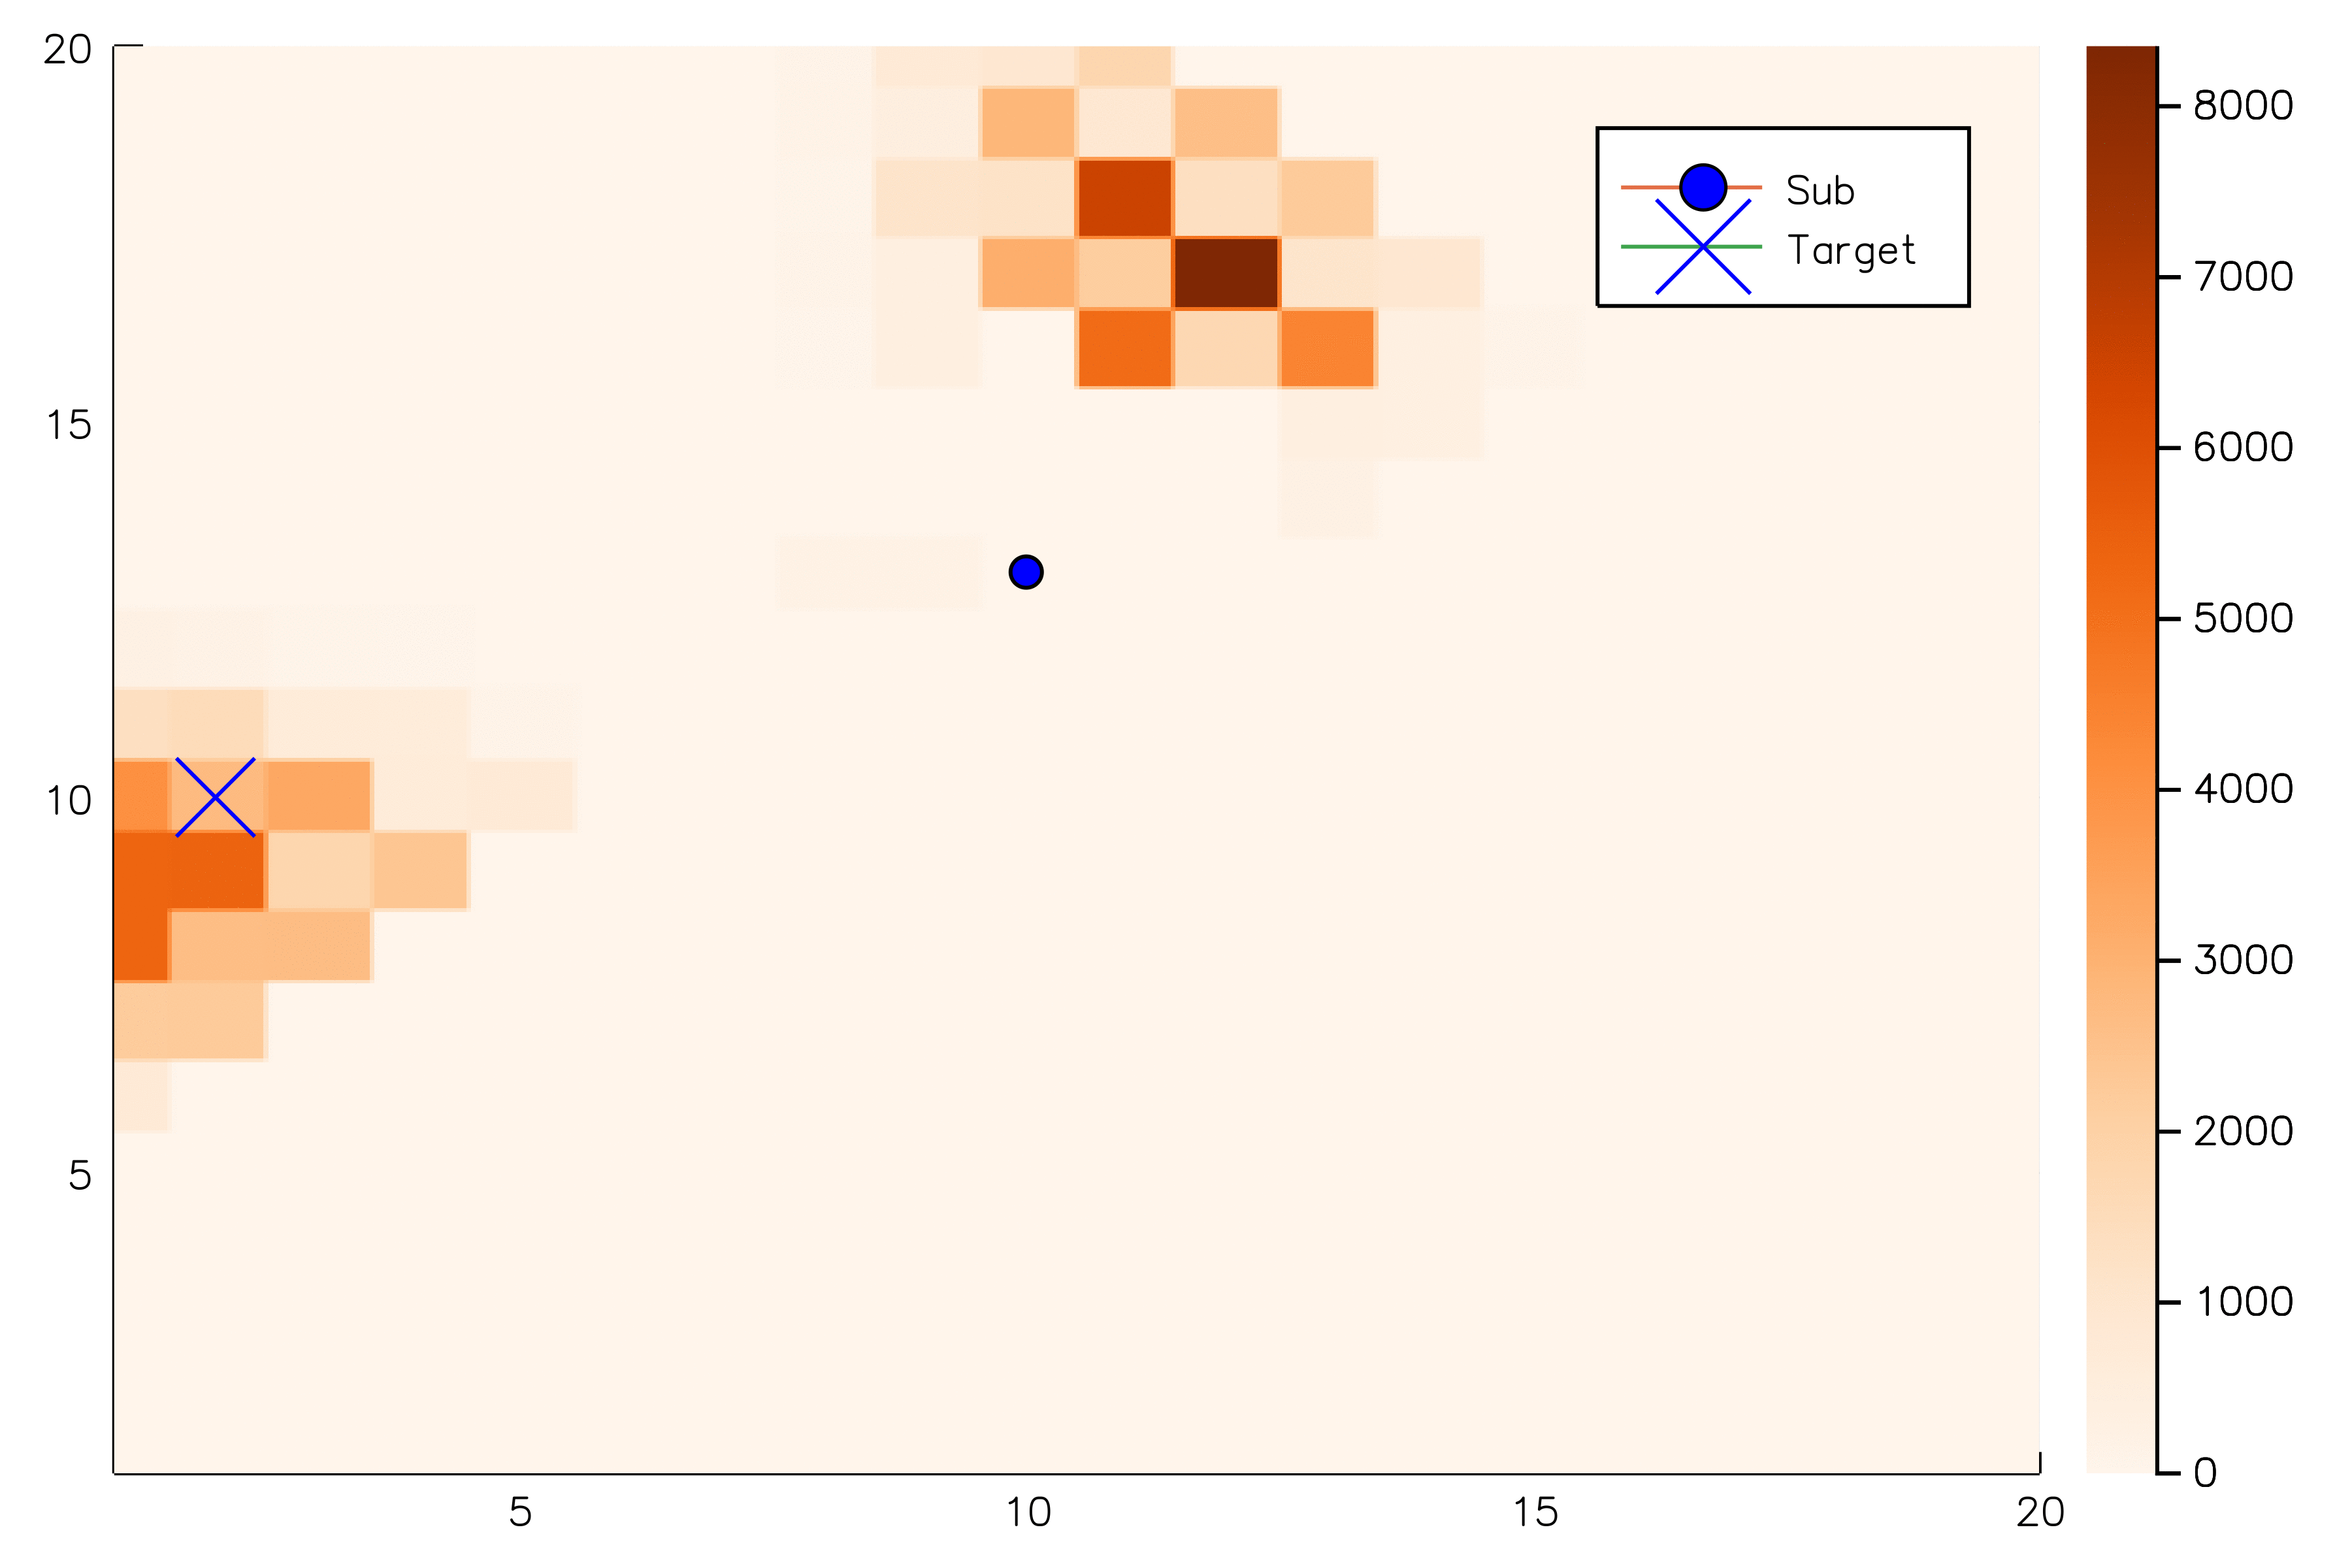
\includegraphics[width=0.6\linewidth]{media/subhunt.png}
    \caption[Sub Hunt problem]{Sub Hunt benchmark. The color of each location square shows the number of belief particles containing the target at that location. In this case, the sub has incorrectly concluded that, with high probability, the target is moving towards the east and is chasing that belief concentration.}
    \label{fig:subhunt}
\end{figure}


\subsection{Van Der Pol Tag} \label{sec:vdptag}

\begin{figure}[bth]
    \begin{subfigure}{0.48\linewidth}
        \centering
        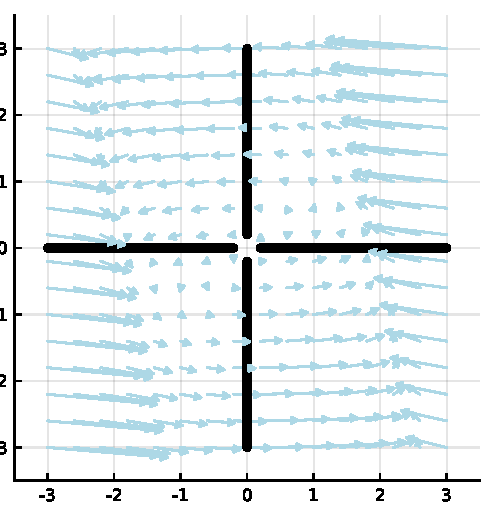
\includegraphics[height=2in]{media/vdp_quiver.pdf}
        \caption{Van Der Pol Dynamics. The arrows show the target differential equation, and the thick black lines represent the barriers.}
    \end{subfigure}
    \hfill
    \begin{subfigure}{0.48\linewidth}
        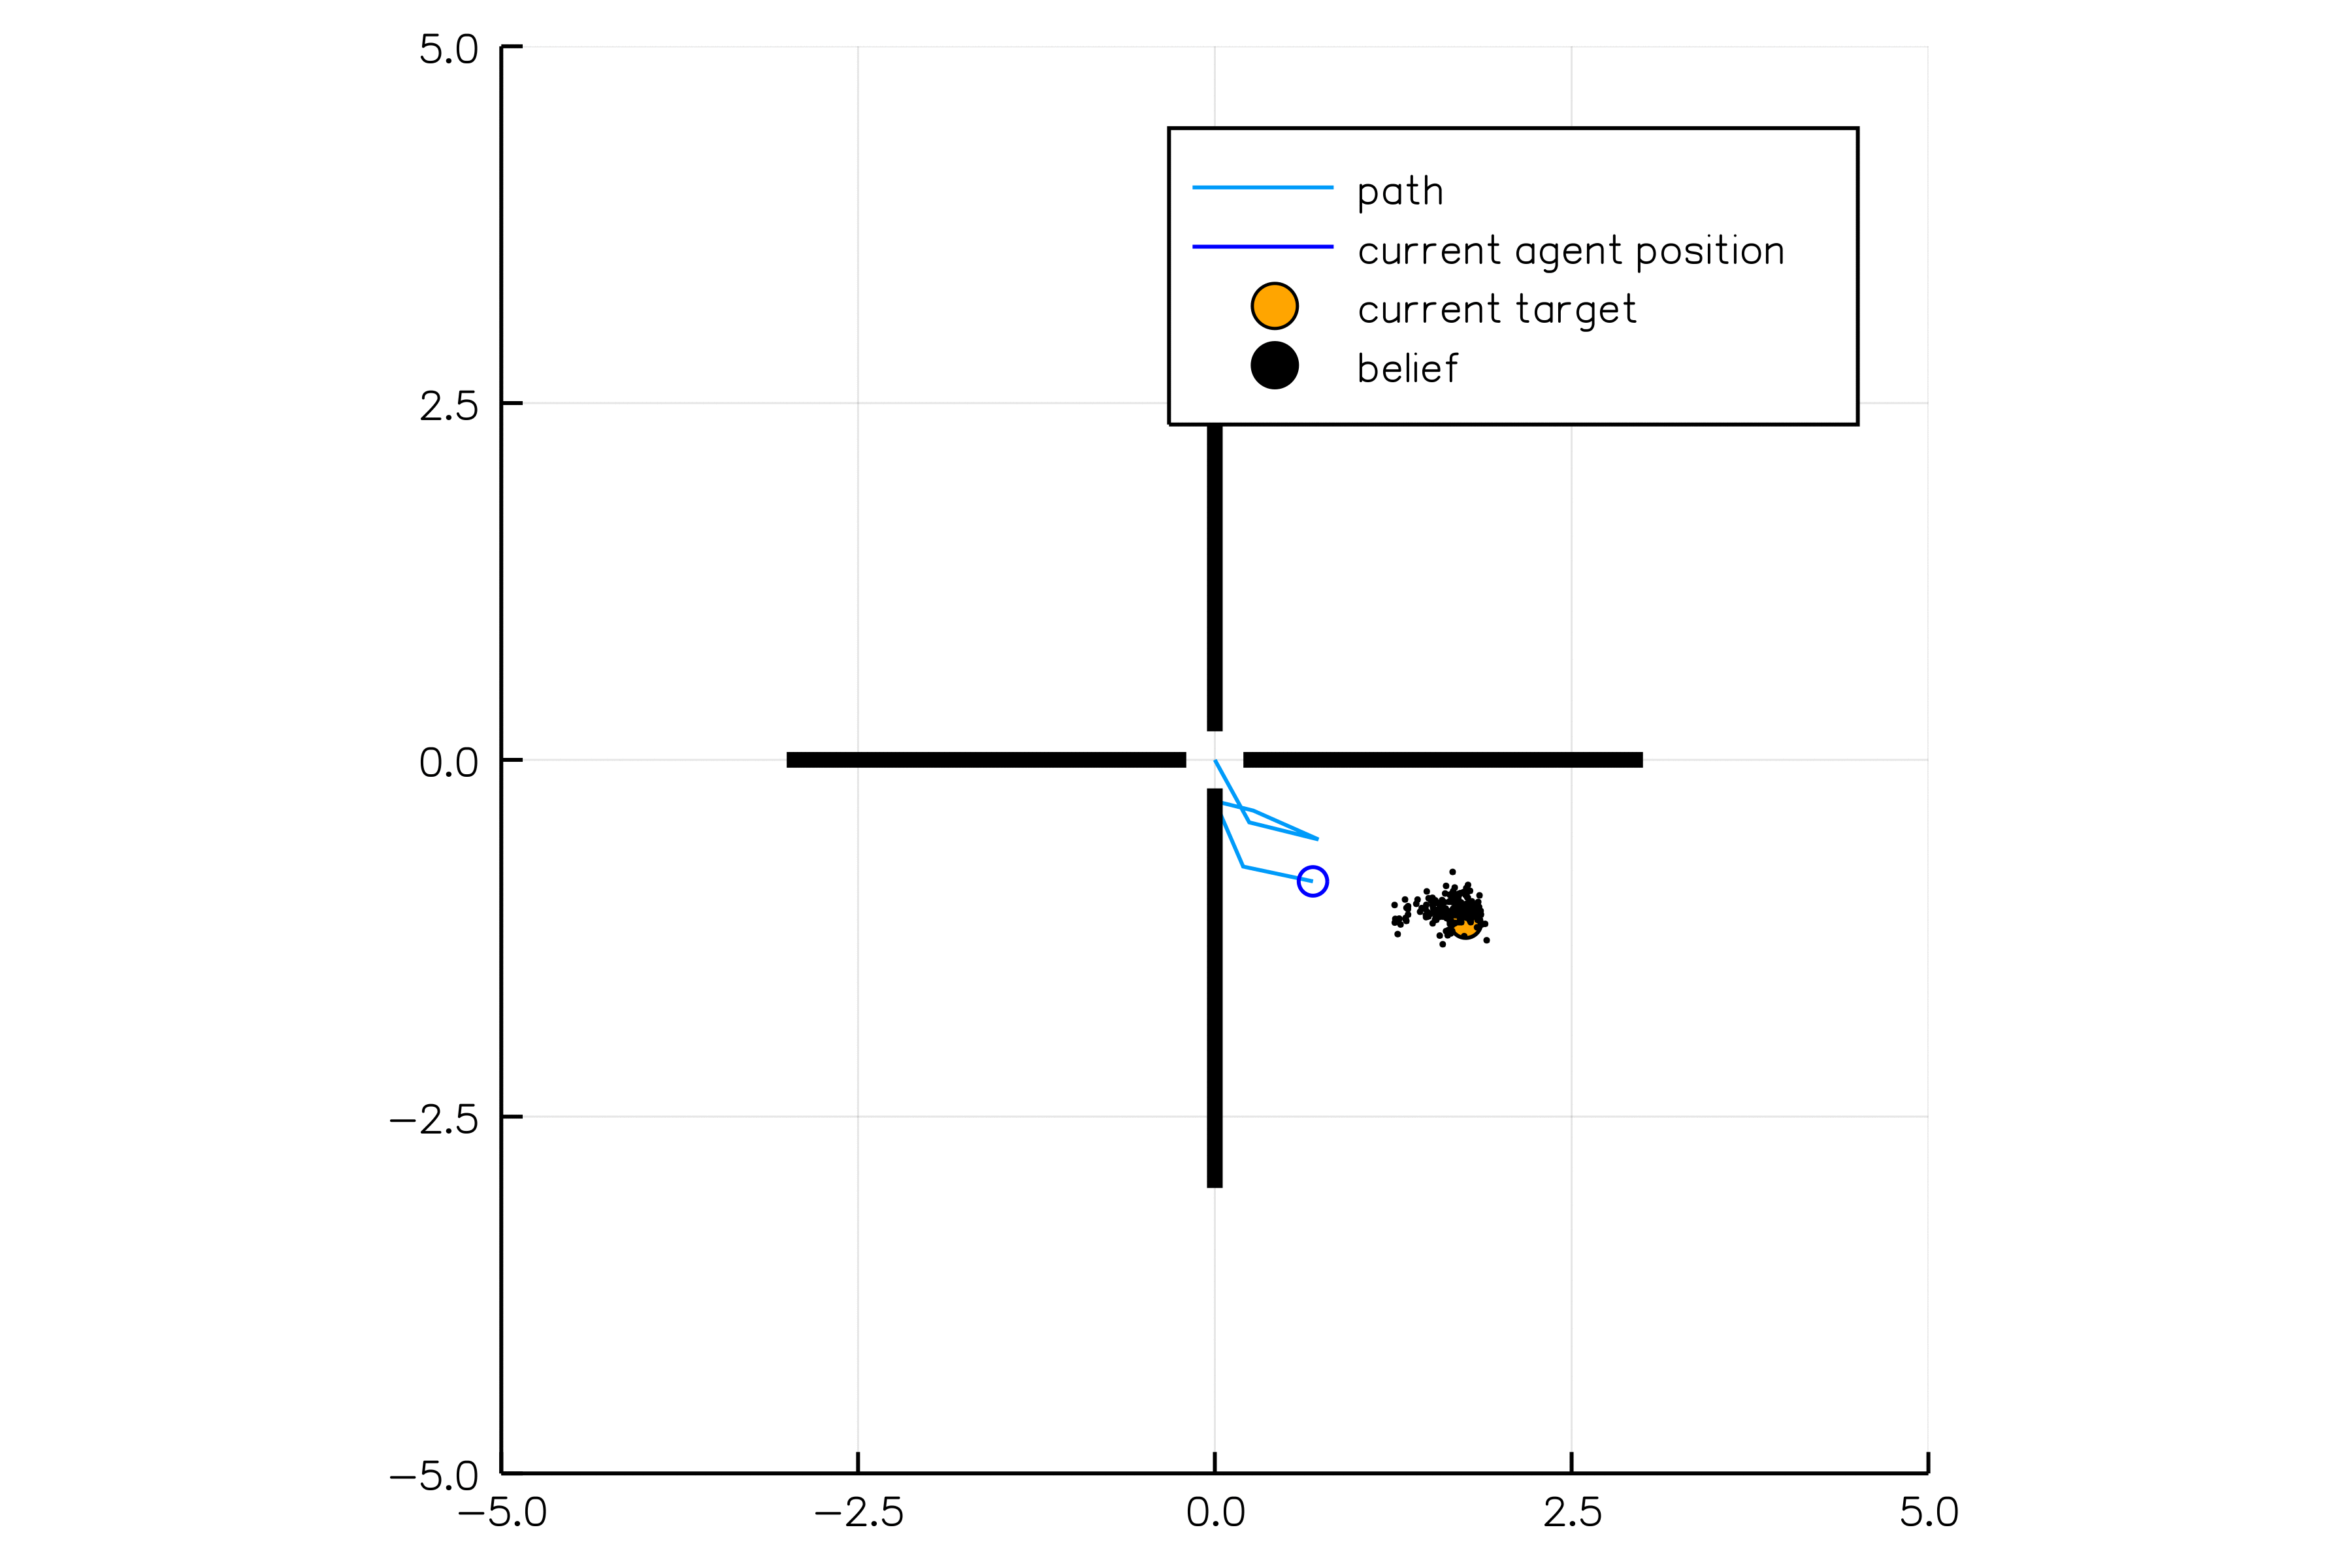
\includegraphics[height=2in]{media/vdptag.png}
        \caption{Van Der Pol Tag. The agent attempts to tag the target, but cannot pass through barriers.}
    \end{subfigure}
    \caption[Van Der Pol tag problem]{Van Der Pol tag problem}
    \label{fig:vdp}
\end{figure}


The final experimental problem is called Van Der Pol tag and has continuous state, action, and observation spaces.
In this problem an agent moves through 2D space to try to tag a target ($\mathcal{S}=\reals^4$) that has a random unknown initial position in $[-4, 4]\times[-4,4]$.
The agent always travels at the same speed, but chooses a direction of travel and whether to take an accurate observation ($\mathcal{A} = [0, 2\pi)\times\{0,1\}$).
The observation again consists of 8 beams ($\ospace=\reals^8$) that give measurements to the target.
Normally, these measurements are too noisy to be useful ($\sigma=5$), but, if the agent chooses an accurate measurement with a cost of \num{5}, the observation has low noise ($\sigma=0.1$).
The agent is blocked if it comes into contact with one of the barriers that stretch from \num{0.2} to \num{3.0} in each of the cardinal directions (see \cref{fig:vdp}), while the target can move freely through.
There is a cost of \num{1} for each step, and a reward of \num{100} for tagging the target (being within a distance of \num{0.1}).


The target moves following a two dimensional form of the Van Der Pol oscillation defined by the differential equations%
\begin{equation}
    \dot{x} = \mu \left( x - \frac{x^3}{3} -y \right) \quad \text{ and }\quad \dot{y} = \frac{1}{\mu}x\text{,} \nonumber
\end{equation}
where $\mu=2$.
Gaussian noise ($\sigma=0.05$) is added to the position at the end of each step.
Runge-Kutta fourth order integration is used to propagate the state.

This problem has several challenging features that might be faced in real-world applications.
First, the state transitions are more computationally expensive because of the numerical integration.
Second, the continuous state space and obstacles make it difficult to construct a good heuristic rollout policy, so random rollouts are used.
\Cref{tab:experiments} shows the mean reward for $1000$ simulations of this problem for each solver.
Since a POMCPOW iteration requires less computation than a PFT-DPW iteration, POMCPOW simulates more random rollouts and thus performs slightly better.

\subsection{Multilane}

The final problem for evaluation is the multiple-lane-change problem described in \cref{sec:multilanepomdp}.
Since costly information gathering is not an important part of this problem, POMCP-DPW and POMCPOW have similar performance.
Because it uses a fixed number of scenarios and bounds to control exploration rather than progressive widening and a UCB heuristic, DESPOT is able to make better long term plans and is the most effective in this problem.
It is also important to note that in this problem, the most realistic of the test problems, PFT-DPW performs significantly worse than POMCPOW.

\subsection{Discretization granularity} \label{sec:discgran}

\Cref{fig:disc} shows the performance at different discretization granularities for the Light Dark and Sub Hunt problems.

Since the Light Dark domain has only a single observation dimension, it is easy to discretize.
In fact, POMCP with fine discretization outperforms POMCPOW.
However, discretization is only effective at certain granularities, and this is highly dependent on the solver and possibly hyperparameters.
In the Sub Hunt problem, with its high-dimensional observation, discretization is not effective at any granularity.
In Van Der Pol tag, both the action and observation spaces must be discretized.
Due to the high dimensionality of the observation space, similar to Sub Hunt, no discretization that resulted in good performance was found.

\begin{figure}[htb]
    \centering
    \begin{subfigure}{0.48\linewidth}
        \centering
        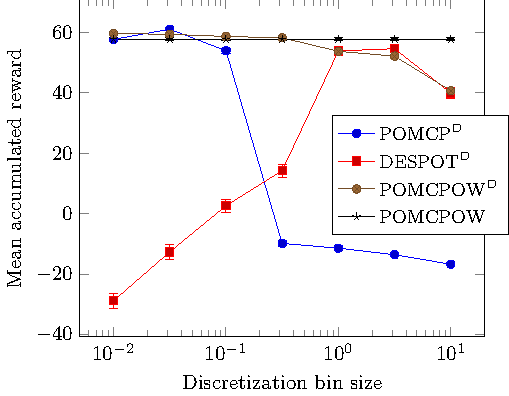
\includegraphics[width=0.97\linewidth]{media/ld_discretization.pdf}
        \caption{Light Dark} \label{fig:lddisc}
    \end{subfigure}
    \begin{subfigure}{0.48\linewidth}
        \centering
        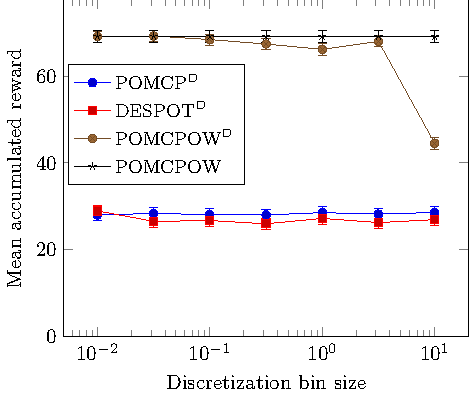
\includegraphics[width=0.9\linewidth]{media/subhunt_discretization.pdf}
        \caption{Sub Hunt}
        \label{fig:shdisc}
    \end{subfigure}

    \caption{Discretization granularity studies} \label{fig:disc}
\end{figure}


\subsection{Hyperparameters} \label{sec:hyper}

\begin{table}[htbp]
    {\centering
\caption{Hyperparameters used in experiments} \label{tab:hyper}

\begin{center}
\begin{tabular}{lrrrrr}
    \toprule
    POMCPOW     & Laser Tag     & Light Dark    & Sub Hunt      & VDP Tag     & Multilane \\
    \midrule
    $c$         & \num{26.0}    & \num{90.0}    & \num{17.0}    & \num{110.0} & \num{8.0} \\
    $k_a$       & --            & --            & --            & \num{30.0}  & -- \\
    $\alpha_a$  & --            & --            & --            & \num{1/30}  & -- \\
    $k_o$       & \num{4.0}     & \num{5.0}     & \num{6.0}     & \num{5.0}   & \num{4.5} \\
    $\alpha_o$  & \num{1/35}    & \num{1/15}    & \num{1/100}   & \num{1/100} & \num{1/10} \\
    \midrule
    PFT-DPW     & Laser Tag     & Light Dark    & Sub Hunt      & VDP Tag     & Multilane \\
    \midrule
    $m$         & \num{20}      & \num{20}      & \num{20}      & \num{20}    & \num{15} \\
    $c$         & \num{26.0}    & \num{100.0}   & \num{100.0}   & \num{70.0}  & \num{8.0} \\
    $k_a$       & --            & --            & --            & \num{20.0}  & -- \\
    $\alpha_a$  & --            & --            & --            & \num{1/25}  & -- \\
    $k_o$       & \num{4.0}     & \num{4.0}     & \num{2.0}     & \num{8.0}   & \num{4.5} \\
    $\alpha_o$  & \num{1/35}    & \num{1/10}    & \num{1/10}    & \num{1/85}  & \num{1/10} \\
    \bottomrule

\end{tabular}

    \vspace{1mm}
    \footnotesize{For problems with discrete actions, all actions are considered and $k_a$ and $\alpha_a$ are not needed.}
\end{center}
    }
\end{table}

Hyperparameters for POMCPOW and PFT-DPW were chosen using the cross entropy method \cite{mannor2003cross}, but exact tuning was not a high priority and some parameters were re-used across solvers so the parameters may not be perfectly optimized.
The values used in the experiments are shown in \cref{tab:hyper}. 
There are not enough experiments to draw broad conclusions about the hyperparameters, but it appears that performance is most sensitive to the exploration constant, $c$.

The values for the observation widening parameters, $k_o$ and $\alpha_o$, were similar for all the problems in this work.
A small $\alpha_o$ essentially limits the number of observations to a static number $k_o$, resulting in behavior reminiscent of sparse UCT \cite{browne2012survey}, preventing unnecessary widening and allowing the tree to grow deep.
This seems to work well in practice with the branching factor ($k_o$) set to values between \num{2} and \num{8}, and suggests that it may be sufficient to limit the number of children to a fixed number rather than do progressive widening in a real implementation.

\section{Discussion}

The results in this chapter clearly show that the previous leading online solvers are unable to adequately solve POMDPs with continuous observation spaces where exploration is important.
In particular, \cref{thm:qmdp} explains why these methods behave similarly to QMDP.
POMCPOW and PFT-DPW overcome this limitation and outperform QMDP.
Though POMCPOW only performs strictly best on one of the problems in \cref{sec:experiments}, it performs very well on all of them, so it might be considered the best overall algorithm in these tests.

However there are still several shortcomings.
First, I have not proven analytically that POMCPOW or PFT-DPW converges toward the optimal solution.
% , and, given the complexity of the proof for DPW in the fully-observable case \cite{auger2013continuous}, this seems to be a relatively challenging task.
Second, double progressive widening is made more difficult in practice because of its tuning parameters.
Third, the results from the Multilane experiment shows that DESPOT is able to find significantly better plans in more realistic problems.
Thus, much work remains along this trajectory.
DESPOT has several attractive attributes compared to the new algorithms presented here.
In particular, its use of a fixed number of scenarios to control widening, and bounds to control exploration may make it more amenable to analysis and allow it to perform better in practice.
Extending DESPOT to handle continuous observation spaces seems to be a promising future direction.

In order to make this type of research much easier, the Stanford intelligent systems lab has created a software framework called POMDPs.jl which provides a standard interface for expressing problems and tools for rapidly prototyping and evaluating new algorithms using the Julia programming language.
This framework is the subject of the next chapter.

\chapter{POMDPs.jl: A Framework for Sequential Decision Making under Uncertainty} \label{chap:pomdpsjl}

Since exact optimal solutions to POMDPs can rarely be attained, most research into solving realistic problems involves empirical comparison between solution techniques.
Sharing solver software between researchers can greatly improve speed and quality of this work.
This chapter describes the POMDPs.jl software package created by the Stanford Intelligent Systems Lab (SISL) to make state-of-the-art POMDP solution methods easily accessible to students, researchers, and engineers.
All of the research in \cref{chap:multilane,chap:pomcpow} was conducted using this framework.

\todo{Use cases?}

\section{Challenges for POMDP-solving software}

A successful POMDP software framework must have, at a minimum, the following attributes: speed, flexibility, and ease of use. Achieving all of these attributes simultaneously is a major challenge.

\subsection{Speed}

Since POMDPs are difficult to solve\todo{Make stronger statement about computational complexity}, any computational slowdown such as unnecessary memory allocation or runtime type inference significantly reduces the maximum problem size that the framework can handle.
For this reason, POMDP algorithms must be compiled to efficient processor instructions with low overhead.

\subsection{Flexibility}

The set of problems that can be represented as a POMDP is extremely large and there are many possible characteristics that such problems might have.
A good POMDP software framework should try to accommodate as much of this set as possible.
A few of the most important model characteristics to support are outlined below.

\subsubsection{Partial and full observability}

When studying a POMDP problem, it is almost always important to analyze the underlying fully-observable problem.
Thus, a good POMDP framework should have first-class support for MDPs in addition to POMDPs.

\subsubsection{Continuous and discrete problems}

Some POMDPs have a finite number of states, actions, and observations, i.e. $|\sspace| < \infty$, $|\aspace| < \infty$, and $|\ospace| < \infty$.
However, many real world problems, notably robotics problems, are naturally formulated in spaces with uncountably infinite cardinality, e.g. $\sspace = \reals$, $\aspace = \reals$, and $\ospace = \reals$, multi-dimensional vector spaces, e.g. $\sspace = \reals^6$, or hybrid continuous-discrete spaces.
This means that the framework must not be constrained to use integers for state representation, but should be capable of using a range of structures including floating point numbers and arrays.

\subsubsection{Explicit vs generative model representation}

Some POMDP and MDP solution techniques use the explicit probability distributions $\tdist$ and $\odist$ to solve problems.
Thus, a successful framework must include a way to explicitly specify $\tdist$ and $\odist$.
On the other hand, explicitly specifying $\tdist$ and $\odist$ for many realistic problems is exceedingly difficult and tedious, and specifying a generative model is the only practical way to encode the problem.
Thus, a successful framework must also include generative model support.

\subsubsection{Online and offline solvers}

While some POMDP solution techniques seek exact offline solutions to small problems, many larger problems can only be practically solved online.
Thus a good POMDP framework must have first class support for solving offline and efficiently executing a policy online or executing a planner that does significant computation online.

\subsubsection{Policy representation}

The policies that different solution techniques yield can take a variety of forms.
Exact solution techniques typically attempt to find alpha vectors that encode an optimal policy \cite{kaelbling1998planning,kurniawati2008sarsop}, whereas others use finite state machines \cite{bai2010mcvi}.
Newer methods may use neural networks \cite{karkus2017qmdp} or other structures to store policies, so a successful framework must provide a flexible way to represent all of these structures.

\subsection{Ease of Use}

In addition to being flexible and performant, the framework must be easy to use.
It is possible to make a framework that is performant and flexible but so complex that it will not be adopted or will cause much time to be wasted in understanding and implementation.
For the framework to be considered a success, it must be adopted by the community and serve as an enabler rather than a hindrance to research.

\section{Previous frameworks}

A number of frameworks exist for solving sequential decision problems.
However, most frameworks are written from a reinforcement learning perspective and hence only support either fully observable problems or problems where the state is fully observable, or environments that can generate observations but do not provide access to the Markov state structure of the problem.
Examples from this class are BURLAP~\cite{diuk2008object}, RLPy~\cite{geramifard2015rlpy}, and rllab~\cite{duan2016benchmarking}.
The most closely related frameworks to POMDPs.jl are APPL~\citep{appl}, AI-Toolbox~\citep{aitoolbox}, and ZMDP~\citep{zmdp} in that they explicitly represent the state and partial observability.
\todo{Check if BURLAP and ai toolbox actually do what I say}

APPL is the most widely used and up to date of these POMDP frameworks.
It is written efficiently in C++ and is excellent from a speed perspective.
However, it has several shortcomings in terms of flexibility and ease of use.
First, though all of the solvers in APPL support the POMDPX file format for discrete, explicit problem definitions, flexibility is limited because there is not a unified interface for defining generative models or continuous explicit models.
Second, prototyping problems and solvers in this framework is relatively time consuming and complex, making it difficult to use.
Specifically, the POMDPX file format is based on XML and is difficult for humans to write directly, so, in most cases, custom scripts must be written to create the files, and solvers and generative models written in C++ have higher development time costs than those written in a higher level language.

\todo{Check to make sure there is not a unified distribution}
\todo{Get quote from APPL}

Though much research progress has been made with these frameworks, POMDPs.jl offers several significant improvements.

\section{Architecture}

POMDPs.jl is designed to facilitate communication between different people performing three actions: defining problems, writing solver software, and running simulation experiments.
The same person will often operate in two or even all three of these roles, but will nearly always bring in some tools written by others.

The framework derives its solutions to the challenges outlined above primarily through the use of the Julia language itself \cite{bezanson2017julia}.
Julia is just-in-time compiled using the state-of-the art LLVM compiler framework, giving it speed comparable to traditional compiled languages such as C and C++.
However, unlike other compiled languages, it has many features that make numerical software development easier and faster.
For example, like Python, it is dynamically typed, has a powerful and flexible type system, and uses a modern, convenient syntax with features like list comprehensions, and, like Matlab, it has built-in efficient multidimensional arrays and linear algebra.
The makes meeting the flexibility and ease-of-use goals much easier.

\todo{cite LLVM}
\todo{Make sure Julia is dynamically typed}

This section describes some of the concepts used in the framework before outlining the interface itself.

\subsection{Concepts}

To fulfill each of the roles mentioned above, a programmer implements one or more classes that concretely represent concepts used to describe POMDP solving.
The problem writer creates a concrete subtype of the \texttt{POMDP} or \texttt{MDP} abstract classes to represent a problem, the simulator writer creates a \texttt{Simulator} type to run simulations, and the solver writer creates a \texttt{Solver} subtype to run computations offline, and a \texttt{Policy} subtype to execute a policy online.

In POMDPs.jl the term ``Belief'' is used to mean any structure that encodes the information needed to execute the policy.
For instance, if the policy is encoded as a set of alpha vectors, the belief takes its usual meaning as an explicit probability distribution over the states; for an online solver like POMCP, it must generate states for the tree search; and for a finite-state-machine policy like the one created by MCVI, it is simply the id of the current node.
An \texttt{Updater} in POMDPs.jl is an object that defines how information from new observations is integrated into the belief.
For example, if the belief is a probability distribution, the updater would apply Bayes rule or an approximation.
Since the belief is often closely related to the policy, the solver writer will often implement the \texttt{Updater}, however generic updaters such as particle filters are also available.
\Cref{fig:concepts} shows the three role concepts and some of the associated abstract types and interface functions.

\begin{figure}[htpb]
    \centering
    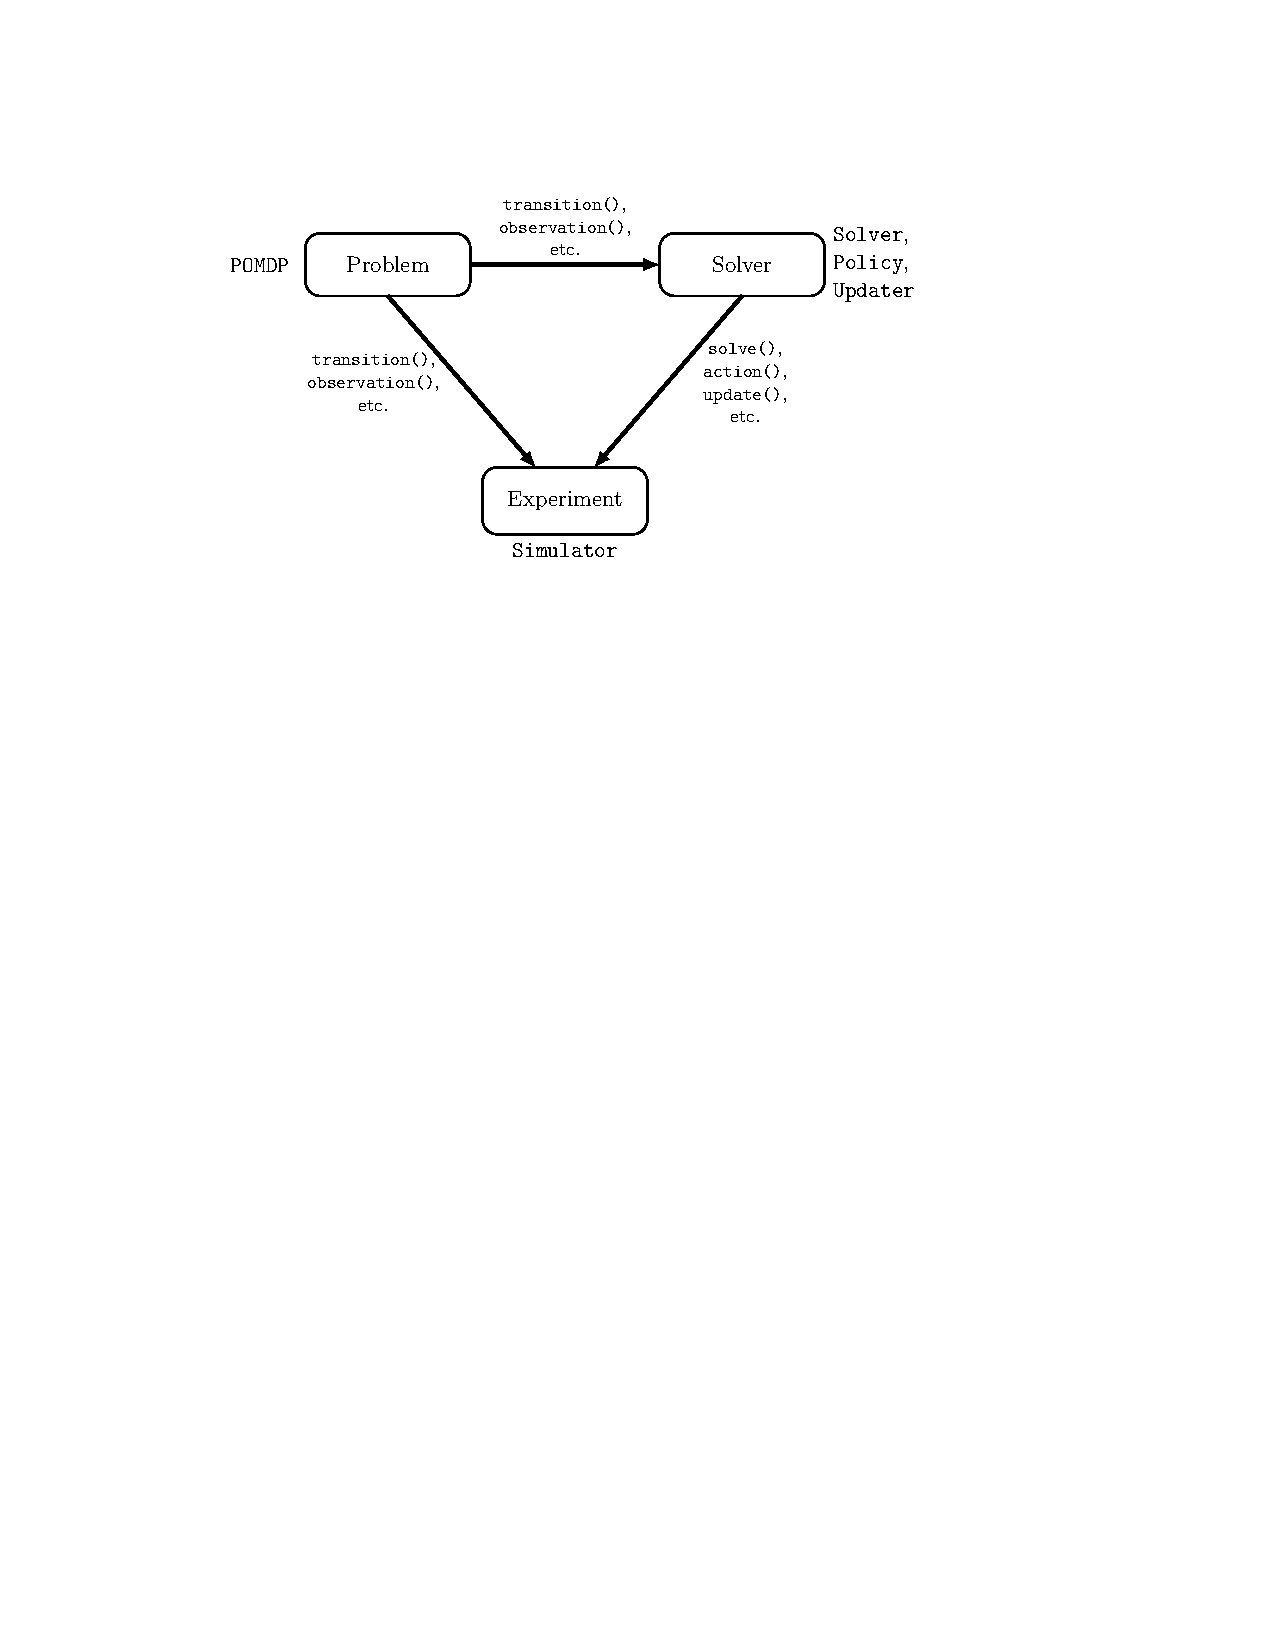
\includegraphics[width=0.8\linewidth]{media/arch.pdf}
    \caption[POMDPs.jl concepts]{POMDPs.jl concepts. POMDPs.jl facilitates communication between people in three roles. The abstract types are shown beside each node and some of the interface functions are shown between the nodes. The arrows indicate which roles use code from which other roles.}
    \label{fig:concepts}
\end{figure}

\subsection{Interfaces}

The behavior of POMDPs.jl objects is defined by implementing methods of interface functions.
Implementing interface functions serves as an alternative to writing configuration files such as POMDPX files or specifications in purpose-built languages like RDDL~\cite{sanner2010rddl} in previous frameworks.
For example the problem writer may implement a method of the \texttt{reward} function that returns the reward given a problem instance, state and action.
Julia will call the correct \texttt{reward} method for the problem type based on its multiple dispatch system \cite{bezanson2017julia}.
Similarly, an \texttt{Updater} should have a corresponding \texttt{update} method that returns a new belief given an updater object, previous belief, action, and observation.
The complete interface is not listed here, but is available in the online documentation.

In POMDPs.jl, states, actions, observations, beliefs, and distributions can be represented by objects of any type as long as the appropriate interface methods are implemented.
This provides the flexibility needed to represent continuous or discrete problems.
Packages in the Julia ecosystem provide convenient and efficient types for common state representations, such as small fixed-size vectors.

One flexibility goal that has not been met by previous frameworks is support of both generative and explicit problem definitions.
For example, in APPL, all solvers can handle POMDPX problem specification for explicit definitions, but the MCVI and DESPOT solvers use different interfaces for generative problems, and there is no way to represent continuous problems explicitly.
POMDPs.jl overcomes this challenge by exposing both an explicit interface and generative interface that can be mixed.
If the necessary parts of the explicit interface are implemented for a problem, POMDPs.jl will automatically provide the generative interface functions for the problem.
The interface relationships are illustrated in \cref{fig:interfaces}.
Implementations of all of the interface functions are not strictly required; if the minimum set of functions used by a solver or simulator are implemented for a problem, then that solver or simulator will work with that problem.

\begin{figure}[htpb]
    \centering
    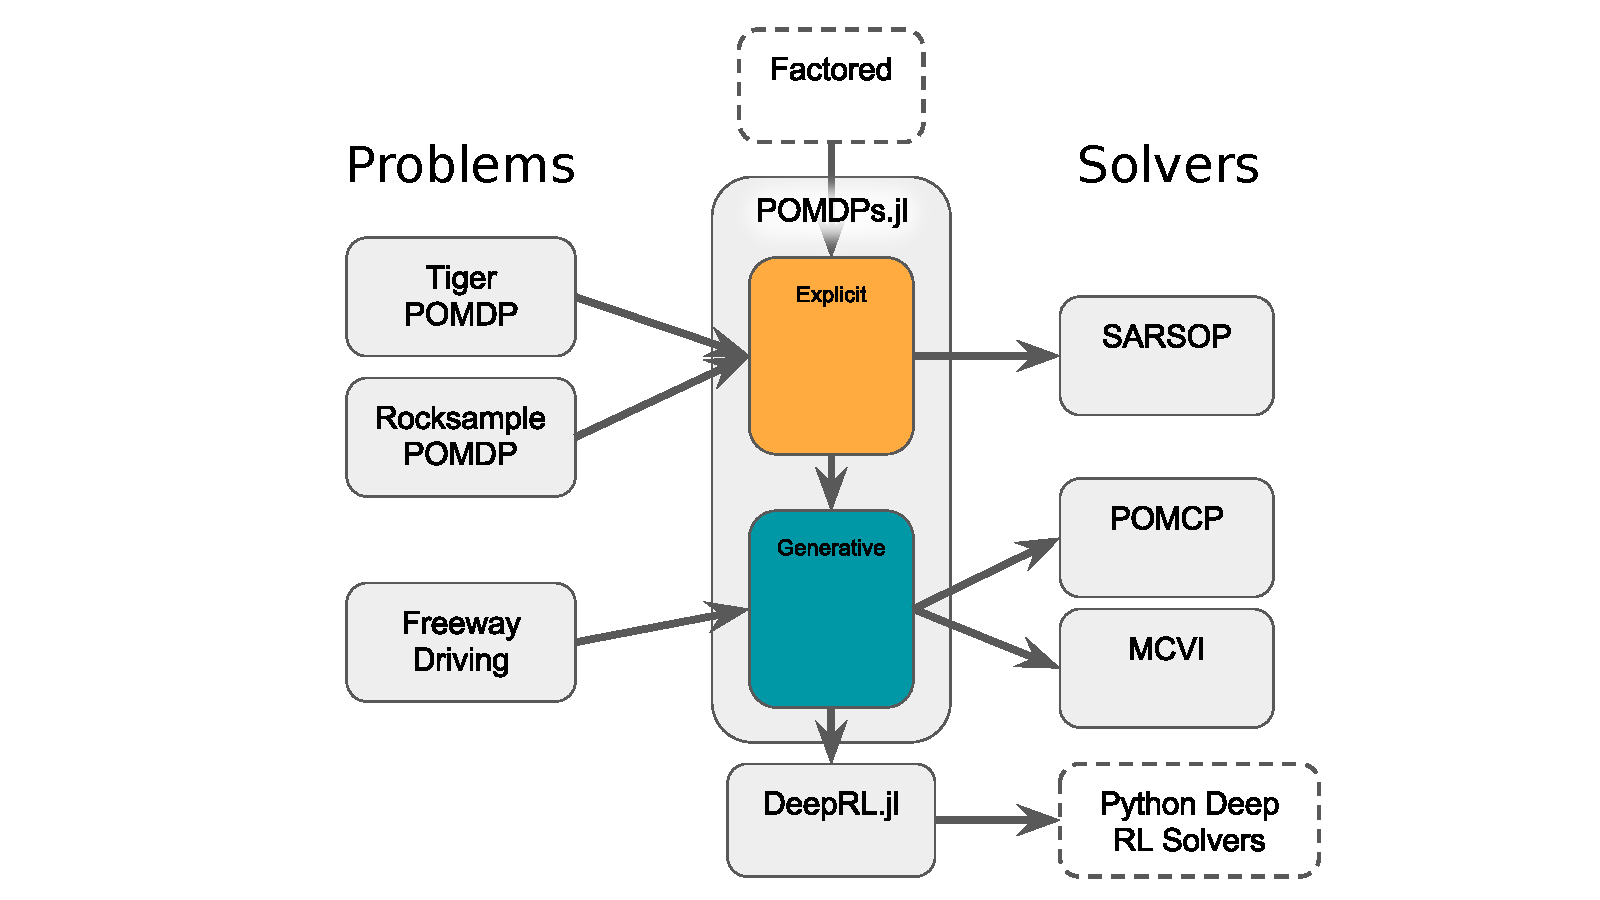
\includegraphics[width=0.8\linewidth]{media/interfaces.pdf}
    \caption{POMDPs.jl interfaces}
    \label{fig:interfaces}
\end{figure}

Because of the interface's flexibility, expressing which interface functions a problem-writer should implement, giving helpful error messages, and even checking whether a sufficient portion of the interface has been implemented is a complex challenge.
For example, suppose a user intends to implement a complex problem that cannot easily be expressed with an explicit definition and intends to use a solver that only requires functions from the generative interface.
If POMDPs.jl advises this user to implement functions from the explicit interface, he or she will conclude that expressing the problem is difficult or impossible.
This complexity drove the development of an interface and framework for dynamically specifying requirements and dependencies and generating helpful reports for users.
In this requirements framework, built with Julia's powerful metaprogramming features, solver and simulator writers declare the requirements for their algorithm, which may be based on solver options, and problem writers can check which of the requirements have been satisfied by their problem implementation.
Examples of the output of this system are shown in \cref{fig:requirements}.

\begin{figure}[htpb]
    \centering
    \begin{subfigure}[b]{0.48\textwidth}
    \begin{center}
        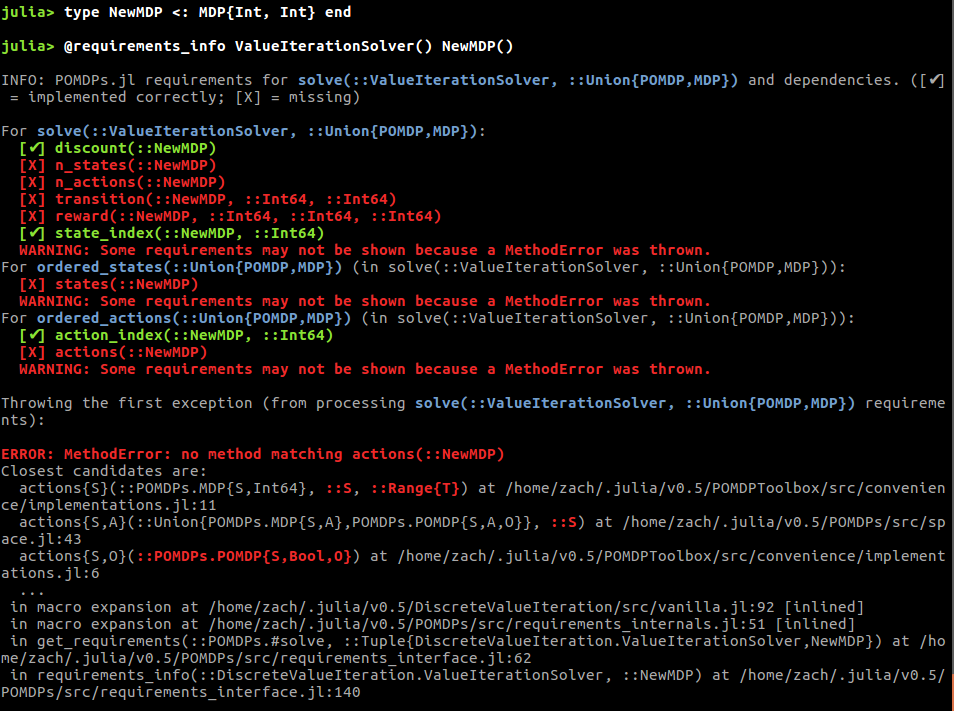
\includegraphics[width=\textwidth]{media/requirements_info_new.png}
    \end{center}
    \caption{New problem with no methods}
    \end{subfigure}
    \hfill
    \begin{subfigure}[b]{0.48\textwidth}
    \begin{center}
        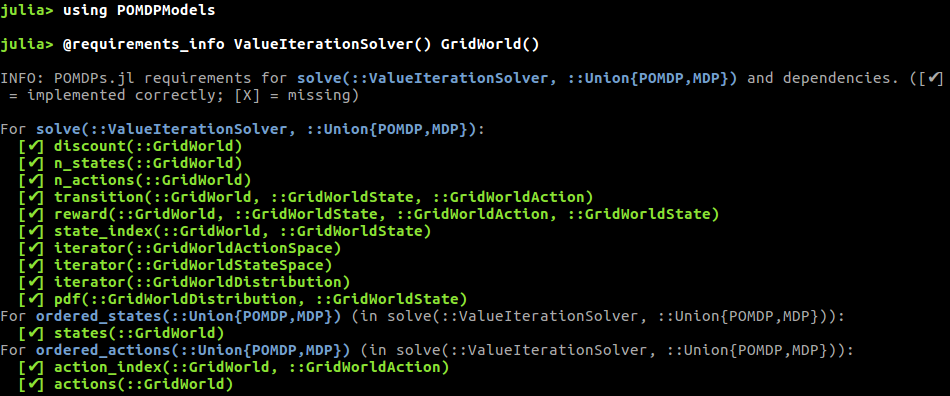
\includegraphics[width=\textwidth]{media/requirements_info_gw.png}
    \end{center}
    \caption{Fully implemented problem}
    \end{subfigure}
     
    \caption[POMDPs.jl requirements example]{POMDPs.jl requirements example output for the value iteration solver}
    \label{fig:requirements}
\end{figure}

\section{Examples}

\chapter{Summary and Future Work}

In order to realize benefits of autonomous transportation, the control systems of autonomous vehicles must be safe.
However, if this safety brings too great a sacrifice in efficiency, the vehicles will not be adopted as widely or be as useful.
This thesis investigated approaches for improving safety while sacrificing minimal efficiency, specifically by proposing better methods for handling the uncertainty inherent in the environment autonomous vehicles operate in.
In addition, the thesis proposed improved algorithms for solving the optimization problems that arise from vehicle control problems
Finally, it described the software framework created to make education and research collaboration in this area easier.
The remainder of this chapter reviews the specific contributions of this thesis and outlines potential future research directions.

\section{Contributions and Summary}

The first contribution (\cref{chap:uav}) is an investigation into the \textbf{combination of trusted resolution logic and optimization} for UAV collision avoidance.
Simple TRL has the advantage that guarantees about its operation are relatively easy to certify.
However, a comparison between simple TRL alone and MDP optimization shows that there is a price in terms of both safety and efficiency accrued for using the TRL.
To reduce this price, two methods for combining the approaches are investigated.
The first is to use an MDP policy to dynamically adjust the parameters of the TRL that govern its conservativeness.
The second is to use the TRL as a constraint on the actions that the MDP policy can choose.
Simulation experiments show that the second approach is superior.

The second contribution (\cref{chap:multilane}) is a \textbf{study of uncertainty modeling in decision making for autonomous highway lane changing}.
This chapter considered approximate POMDP solutions where the internal states of other drivers are explicitly modeled as a hidden part of the Markov state.
The POMDP solutions are compared with approximate MDP solutions, both assuming full knowledge of the internal state and conservatively modeling state uncertainty as outcome uncertainty.
\textbf{The advantage of POMDP solutions over MDP solutions is clear} in all of the tests, but the relative effectiveness of different POMDP approximations depends greatly on the correlation of the different internal state parameters.
Simulation tests show that when the parameters are highly correlated, since it is easier to estimate the hidden states, even greatly simplified POMDP approximations can achieve performance near the upper bound established by an omnipotent planner.
On the other hand, when there is little or no correlation, POMDP solution methods that include more of the uncertainty in the solution process perform significantly better.
Experiments also characterize the robustness of the algorithms with respect to the parameter distribution.

The third contribution (\cref{chap:pomcpow}) is a pair of \textbf{improved algorithms for solving POMDPs online}.
Previous leading online algorithms have focused on solving discrete problems, and are unable to solve problems with continuous action and observation spaces.
Hence, new algorithms for the continuous domains encountered in the real world are needed.
The first part of this contribution (\cref{sec:pomcpdpw}) is proving that \textbf{a naive application of double progressive widening to the POMCP algorithm will result in suboptimal behavior}.
In particular, in a continuous observation space, it will converge to the QMDP solution because each belief node will degenerate to a single state particle (\cref{thm:qmdp}).
In fact, numerical experiments confirm that all leading online solvers exhibit this behavior.

In response to this suboptimality, two new algorithms are proposed (\cref{sec:pftdpw,sec:pomcpow}).
The first, PFT-DPW, solves an approximation of the belief MDP, while the second, \textbf{POMCPOW}, is an extension of POMCP with double progressive widening and weighted particle filtering.
Numerical experiments (\cref{sec:experiments}) show that these algorithms are able to break the QMDP barrier and hence exhibit performance that is qualitatively superior to previous algorithms.
POMCPOW and PFT-DPW perform similarly on most problems, but on the most realistic problem, a version of the autonomous driving problem from~\cref{chap:multilane}, POMCPOW outperforms PFT-DPW.

The final contribution (\cref{chap:pomdpsjl}) is a software framework, \textbf{POMDPs.jl}, which provides an interface for expressing MDPs and POMDPs and tools for developing and testing solvers.
This framework is unprecedented in its flexibility.
It can represent discrete and continuous MDPs defined by both explicit probability distributions and simulators that provide generative models.
The Julia language also gives solvers written to use the framework speed comparable to previous C++ implementations.

\section{Future Work}

There are many promising directions for future work to proceed from the results presented in this thesis.
The discussion portion of each chapter gives short-term specific extensions to the individual research efforts described therein.
This section gives a broader overview.

The first line of future work involves \textbf{safety constraints}.
Interaction of safety constraints with sequential optimization is explored in \cref{chap:uav} and such constraints are used in \cref{chap:multilane}.
However, the actual constraints used there are very simple.
In real problems, these constraints will need to be more complex, consisting of, for example, linear temporal logic rules~\cite{sadigh2016safe} or results from reachability analysis~\cite{chen2015exact}.
Combining approximate POMDP solutions with these advanced safety constraints to field a reliable system still requires much research.

The second line is focused on \textbf{modeling}. \Cref{chap:uav,chap:multilane} evaluate their findings based on simplistic models of other vehicles.
To solidify the conclusions of this thesis, better data-driven models of human drivers and pilots must be created.
Indeed, significant work has already been done in this area~\cite{schmerling2018multimodal,bhattacharyya2018multi}. 
However, these models are limited in scope, primarily because of the limited data available.
In order to be able to test in more diverse scenarios, more data will need to be collected from the real world, and models that are more data-efficient developed.
Moreover, current planning algorithms will not work efficiently with certain models.
A particular example is that recurrent neural networks with latent states the represent beliefs over internal states~\cite{schmerling2018multimodal} will not work with the POMDP algorithms used in this thesis.
Thus, new algorithms must be developed to work with the new models.

The third direction is continuing the development of better \textbf{POMDP algorithms}.
While the algorithms proposed in \cref{chap:pomcpow} demonstrate better performance than previous algorithms, the shortcomings of this family of algorithms are also apparent.
In particular, algorithms based on MCTS-DPW have many tuning parameters that must be chosen via unreliable hand tuning or time consuming optimization.
In addition, the proof of consistency for MCTS-DPW~\cite{auger2013continuous} is rather tedious, which is one of the reasons that an analytical proof for the optimality of POMCPOW was not attempted for this thesis.
Moreover, the trees produced by these algorithms tend to be shallow, reducing the effective planning horizon.
As seen in the experimental results for the multilane model in \cref{tab:experiments}, DESPOT is able to perform better on more realistic problems because it builds deeper trees and explores based on bounds rather than upper confidence estimates.
DESPOT's fixed number of scenarios may also make analysis easier.
Given these advantages, the particle filter weighting approaches used in PFT-DPW and POMCPOW should be applied to more advance algorithms like DESPOT to enable them to explore in continuous observation spaces.
Furthermore, all of the algorithms discussed in this thesis use a single execution thread. In order to take advantage of modern computing hardware, online parallel algorithms for solving POMDPs must be investigated.

Finally, the problem of controlling autonomous vehicles in continuous, partially observable domains has by no means been solved.
One reason is the weakness of decision-making \textbf{algorithms for continuous spaces} that can handle uncertainty and irregularity.
This thesis focused on continuous state and observation spaces, but the action space is arguably the most difficult context for continuity.
Some research has begun to address this~\cite{seiler2015online,wang2018online}, but these algorithms use only derivative-free optimization techniques that may not scale to high dimensional problems.
In many continuous problems, if history $h_1$ consists of actions and observations near the actions and observations of history $h_2$, the value at $h_1$ will be very close to the value at $h_2$.
This information is not exploited in any of the online solvers discussed in this thesis.
Although some work has been done to use this information in MCTS~\cite{xiao2018memory}, new algorithms that use ideas from optimal control, model predictive control, and motion planning may be much better suited for continuous problems.


% and the end material

\appendix
% 
\chapter{Proof of Theorem 1} \label{sec:proof}

A version of Monte Carlo tree search with double progressive widening has been proven to converge to the optimal value function on fully observable MDPs by \citet{auger2013continuous}.
We use this proof to show that POMCP-DPW converges to the QMDP solution.

First we establish some preliminary definitions taken directly from \citet{auger2013continuous}.

\begin{definition}[Regularity Hypothesis]
    The \emph{Regularity hypothesis} is the assumption that for any $\Delta > 0$, there is a non zero probability to sample an action that is optimal with precision $\Delta$. More precisely, there is a $\theta > 0$ and a $p > 1$ (which remain the same during the whole simulation) such that for all $\Delta > 0$, 
\begin{align}
    Q(ha) \geq Q^*(h)-\Delta \text{ with probability at least } \min(1, \theta \Delta^p)\text{.}
\end{align}
\end{definition}

\begin{definition}[Exponentially sure in $n$]
    We say that some property depending on an integer $n$ is exponentially sure in $n$ if there exists positive constants $C$, $h$, and $\eta$ such that the probability that the property holds is at least $$1-C \exp(-hn^\eta)\text{.}$$
\end{definition}

In order for the proof from \citet{auger2013continuous} to apply, the following four minor modifications to the POMCP-DPW algorithm must be made: 

\begin{enumerate}
    \item Instead of the usual logarithmic exploration, use \emph{polynomial exploration}, that is, select actions based on the criterion
    \begin{equation}
        Q(ha) + \sqrt{\frac{N(h)^{e_d}}{N(ha)}}\text{,}
    \end{equation}
    as opposed to the traditional criterion
    \begin{equation}
        Q(ha) + c \sqrt{\frac{\log N(h)}{N(ha)}}\text{,}
    \end{equation}
    and create a new node for progressive widening when $\lfloor N^\alpha \rfloor > \lfloor (N-1)^\alpha \rfloor$ rather than when the number of children exceeds $k N^\alpha$.

    \item Instead of performing rollout simulations, keep creating new single-child nodes until the maximum depth is reached.

    \item In line~\ref{lin:selecto}, instead of selecting an observation randomly, select the observation that has been visited least proportionally to how many times it has been generated.

    \item Use the depth-dependent coefficient values in Table 1 from \citet{auger2013continuous} instead of choosing static values.
\end{enumerate}

This version of the algorithm will be referred to as ``modified POMCP-DPW''. The algorithm with these changes is listed in \Cref{alg:mpomcpdpw}.

\begin{algorithm}[htb]
    \caption{Modified POMCP-DPW} \label{alg:mpomcpdpw}
    \begin{algorithmic}[1]
        \Procedure{Plan}{$b$}
            \For{$i \in 1:n$}
                \State $s \gets \text{sample from }b$ \label{lin:msample}
                \State $\Call{Simulate}{s, b, d_\text{max}}$
            \EndFor
            \State $\textbf{return } \underset{a}{\argmax}\, Q(ba)$
        \EndProcedure

        \Procedure {ActionProgWiden}{$h$}
            \If{$\lfloor N(h)^{\alpha_{a,d}} \rfloor > \lfloor (N(h)-1)^{\alpha_{a,d}} \rfloor$}
                \State $a \gets \Call{NextAction}{h}$
                \State $C(h) \gets C(h) \cup \{a\}$
            \EndIf
            \State $\textbf{return } \underset{a \in C(h)}{\argmax}\, Q(ha) + \sqrt{\frac{N(h)^{e_d}}{N(ha)}}$
        \EndProcedure

        \Procedure {Simulate}{$s$, $h$, $d$}        
            \If{$d = 0$}
                \State \textbf{return} $0$
            \EndIf
            \State $a \gets \Call{ActionProgWiden}{h}$
            \If{$\lfloor N(ha)^{\alpha_{o,d}} \rfloor > \lfloor (N(ha)-1)^{\alpha_{o,d}} \rfloor$}
                \State $s',o,r \gets G(s,a)$
                \State $C(ha) \gets C(ha) \cup \{o\}$
                \State $M(hao) \gets M(hao) + 1$ \label{lin:gencount}
                \State $\text{append } s' \text{ to } B(hao)$ \label{lin:minsertion}
            \Else
                \State $o \gets \underset{o \in C(ha)}{\argmin}\, N(hao)/M(hao)$
                \State $s' \gets \text{select } s' \in B(hao) \text{ w.p. } \frac{1}{|B(hao)|}$
                \State $r \gets \reward(s,a,s')$
            \EndIf
            \State $total \gets r + \gamma \Call{Simulate}{s', hao, d-1}$
            \State $N(h) \gets N(h)+1$
            \State $N(ha) \gets N(ha)+1$
            \State $Q(ha) \gets Q(ha) + \frac{total - Q(ha)}{N(ha)}$
            \State \textbf{return} $total$
        \EndProcedure
    \end{algorithmic}        
\end{algorithm}

We now define the ``QMDP value'' that POMCP-DPW converges to (this is repeated from the main text of the paper) and prove a preliminary lemma.

\qmdpvalue*
% \begin{definition}[QMDP value]
%      Let $Q_\text{MDP}(s,a)$ be the optimal state-action value function assuming full observability starting by taking action $a$ in state $s$.
%      The \emph{QMDP value} at belief $b$, $Q_\text{MDP}(b,a)$, is the expected value of $Q_\text{MDP}(s,a)$ when $s$ is distributed according to $b$.   
% \end{definition}

\begin{lemma} \label{lem:onestate}
    If POMCP-DPW or modified POMCP-DPW is applied to a POMDP with a continuous observation space and observation probability density functions that are finite everywhere, then each history node in the tree will have only one corresponding state, that is $|B(h)| = 1, M(h)=1\, \forall h$.
\end{lemma}

\begin{proof}
    Since the observation probability density function is finite, each call to the generative model will produce a unique observation with probability 1.
    Because of this, lines~\ref{lin:gencount}~and~\ref{lin:minsertion} of \cref{alg:mpomcpdpw} will only be executed once for each observation.
\end{proof}

We are now ready to restate the theorem from the text.

% \begin{theorem}[Modified POMCP-DPW convergence to QMDP] \label{thm:pqmdp}
% If a bounded-horizon POMDP meets the following conditions: 1) the state and observation spaces are continuous with a finite observation probability density function, and 2) the regularity hypothesis is met, then modified POMCP-DPW will produce a value function estimate, $\hat{Q}$, that converges to the QMDP value for the problem.
% Specifically, there exists a constant $C>0$, such that after $n$ iterations,
% \begin{equation*}
%     \left| \hat{Q}(b,a) - Q_\text{MDP}(b,a) \right| \leq \frac{C}{n^{1/(10d_{\max}-7)}}
% \end{equation*}
% exponentially surely in $n$, for every action $a$.
% \end{theorem}

\qmdp*

The bound on the value estimate error, $\frac{C}{n^{1/(10d_{\max}-7)}}$,
% \begin{equation}
%     \frac{C}{n^{1/(10d_{\max}-7)}}
% \end{equation}
is based on the specific coefficients chosen by \citet{auger2013continuous} and listed in Table 1 of their paper. Alternative bounds may be possible with different coefficient choices. The proof of the theorem is given below.

\begin{proof}
    We prove that modified POMCP-DPW functions exactly as the Polynomial UCT (PUCT) algorithm defined by \citet{auger2013continuous} applied to an augmented fully observable MDP, and hence converges to the QMDP value.
    We will show this by proposing incremental changes to \cref{alg:mpomcpdpw} that do not change its function that will result in an algorithm identical to PUCT.

    Before listing the changes, we define the ``augmented fully observable MDP" as follows: For a POMDP $\mathcal{P} = (\mathcal{S}, \mathcal{A}, \mathcal{T}, \mathcal{R}, \mathcal{O}, \mathcal{Z}, \gamma)$, and belief $b$, the \emph{augmented fully observable MDP}, $\mathcal{M}$, is the MDP defined by $(\mathcal{S}_A, \mathcal{A}, \mathcal{T}_A, \mathcal{R}, \gamma)$, where 
    \begin{equation}
        \mathcal{S}_A = \mathcal{S} \cup \{b\}
    \end{equation}
    and, for all $x, x' \in \mathcal{S}_A$,
    \begin{equation}
        \mathcal{T}_A (x'|x, a) = \begin{cases}
                \mathcal{T} (x' | x, a) & \text{if } x \in \mathcal{S} \\
                \int_S b(s) \mathcal{T} (x' | s, a) ds & \text{if } x = b
        \end{cases}
    \end{equation}
    This is simply the fully observable MDP augmented with a special state representing the current belief.
    It is clear that the value function for this problem, $Q_\mathcal{M}(b, a)$, is the same as the QMDP value for the POMDP, $Q_\text{MDP}(b,a)$.
    Thus, by showing that modified POMCP-DPW behaves exactly as PUCT applied to $\mathcal{M}$, we show that it estimates the QMDP values.

    % For the above definition, we assume the state space is integrable. Is that ok without stating?

    Consider the following modifications to \cref{alg:mpomcpdpw} that do not change its behavior when the observation space is continuous:

    \begin{enumerate}
        \item Eliminate the state count $M$. \emph{Justification}: By \cref{lem:onestate}, its value will be 1 for every node.
        \item Remove $B$ and replace with a mapping $H$ from each node to a state of $\mathcal{M}$; define $H(b) = b$. \emph{Justification}: By \cref{lem:onestate}, $B$ always contains only a single state, so $H$ contains the same information.
        \item Generate states and rewards with $G_\mathcal{M}$, the generative model of $\mathcal{M}$, instead of $G$. \emph{Justification}: Since the state transition model for the fully observable MDP is the same as the POMDP, these are equivalent for all $s \in \mathcal{S}$.
        \item Remove the $s$ argument of \textproc{Simulate}. \emph{Justification}: The sampling in line~\ref{lin:msample} is done implicitly in $G_\mathcal{M}$ if $h=b$, and $s$ is redundant in other cases because $h$ can be mapped to $s$ through $H$.
    \end{enumerate}

    The result of these changes is shown in \cref{alg:c}. It is straightforward to verify that this algorithm is equivalent to PUCT applied to $\mathcal{M}$.
    Each observation-terminated history, $h$, corresponds to a PUCT ``decision node'', $z$, and each action-terminated history, $ha$, corresponds to a PUCT ``chance node'', $w$.
    In other words, the observations have no meaning in the tree other than making up the histories, which are effectively just keys to or aliases for the state nodes.
    
    Since PUCT is guaranteed by Theorem 1 of \citet{auger2013continuous} to converge to the optimal value function of $\mathcal{M}$ exponentially surely, POMCP-DPW is guaranteed to converge to the QMDP value exponentially surely, and the theorem is proven.

\begin{algorithm}[htb]
    \caption{Modified POMCP-DPW on a continuous observation space} \label{alg:c}
    \begin{algorithmic}[1]
        \Procedure{Plan}{$b$}
            \For{$i \in 1:n$}
                \State $\Call{Simulate}{(b), d_\text{max}}$
            \EndFor
            \State $\textbf{return } \underset{a}{\argmax}\, Q(ha)$
        \EndProcedure

        \Procedure {ActionProgWiden}{$h$}
            \If{$\lfloor N(h)^{\alpha_{a,d}} \rfloor > \lfloor (N(h)-1)^{\alpha_{a,d}} \rfloor$}
                \State $a \gets \Call{NextAction}{h}$
                \State $C(h) \gets C(h) \cup \{a\}$
            \EndIf
            \State $\textbf{return } \underset{a \in C(h)}{\argmax}\, Q(ha) + \sqrt{\frac{N(h)^{e_d}}{N(ha)}}$
        \EndProcedure

        \Procedure {Simulate}{$h$, $d$}        
            \If{$d = 0$}
                \State \textbf{return} $0$
            \EndIf
            \State $a \gets \Call{ActionProgWiden}{h, d}$
            \If{$\lfloor N(ha)^{\alpha_{o,d}} \rfloor > \lfloor (N(ha)-1)^{\alpha_{o,d}} \rfloor$}
                \State $\cdot, o, \cdot \gets G(H(h), a)$
                \State $H(hao),r \gets G_\mathcal{M}(H(h),a)$
                \State $C(ha) \gets C(ha) \cup \{o\}$
            \Else
                \State $o \gets \underset{o \in C(ha)}{\argmin}\, N(hao)$
                \State $r \gets \reward(H(h), a, H(hao))$
            \EndIf
            \State $total \gets r + \gamma \Call{Simulate}{hao, d-1}$
            \State $N(h) \gets N(h)+1$
            \State $N(ha) \gets N(ha)+1$
            \State $Q(ha) \gets Q(ha) + \frac{total - Q(ha)}{N(ha)}$
            \State \textbf{return} $total$
        \EndProcedure
    \end{algorithmic}
\end{algorithm}

\end{proof}

\begin{remark}
    One may object that multiple histories may map to the same state through $H$, and thus the history nodes in a modified POMCP-DPW tree are not equivalent to state nodes in the PUCT tree. In fact, the PUCT algorithm does not check to see if a state has previously been generated by the model, so it may also contain multiple decision nodes $z$ that correspond to the same state. Though this is not explicitly stated by the authors, it is clear from the algorithm description, and the proof still holds.
\end{remark}

% \include{appendix2}
% \include{appendix3}


% bibliography.tex should include either 
% \bibliographystyle{...}
% \bibliography{mythesis}
% or some other way of doing the bibliography
% \include{bibliography}

\printbibliography

\end{document}
